% Options for packages loaded elsewhere
\PassOptionsToPackage{unicode}{hyperref}
\PassOptionsToPackage{hyphens}{url}
%
\documentclass[
]{book}
\usepackage{amsmath,amssymb}
\usepackage{lmodern}
\usepackage{iftex}
\ifPDFTeX
  \usepackage[T1]{fontenc}
  \usepackage[utf8]{inputenc}
  \usepackage{textcomp} % provide euro and other symbols
\else % if luatex or xetex
  \usepackage{unicode-math}
  \defaultfontfeatures{Scale=MatchLowercase}
  \defaultfontfeatures[\rmfamily]{Ligatures=TeX,Scale=1}
\fi
% Use upquote if available, for straight quotes in verbatim environments
\IfFileExists{upquote.sty}{\usepackage{upquote}}{}
\IfFileExists{microtype.sty}{% use microtype if available
  \usepackage[]{microtype}
  \UseMicrotypeSet[protrusion]{basicmath} % disable protrusion for tt fonts
}{}
\makeatletter
\@ifundefined{KOMAClassName}{% if non-KOMA class
  \IfFileExists{parskip.sty}{%
    \usepackage{parskip}
  }{% else
    \setlength{\parindent}{0pt}
    \setlength{\parskip}{6pt plus 2pt minus 1pt}}
}{% if KOMA class
  \KOMAoptions{parskip=half}}
\makeatother
\usepackage{xcolor}
\usepackage{color}
\usepackage{fancyvrb}
\newcommand{\VerbBar}{|}
\newcommand{\VERB}{\Verb[commandchars=\\\{\}]}
\DefineVerbatimEnvironment{Highlighting}{Verbatim}{commandchars=\\\{\}}
% Add ',fontsize=\small' for more characters per line
\usepackage{framed}
\definecolor{shadecolor}{RGB}{248,248,248}
\newenvironment{Shaded}{\begin{snugshade}}{\end{snugshade}}
\newcommand{\AlertTok}[1]{\textcolor[rgb]{0.94,0.16,0.16}{#1}}
\newcommand{\AnnotationTok}[1]{\textcolor[rgb]{0.56,0.35,0.01}{\textbf{\textit{#1}}}}
\newcommand{\AttributeTok}[1]{\textcolor[rgb]{0.77,0.63,0.00}{#1}}
\newcommand{\BaseNTok}[1]{\textcolor[rgb]{0.00,0.00,0.81}{#1}}
\newcommand{\BuiltInTok}[1]{#1}
\newcommand{\CharTok}[1]{\textcolor[rgb]{0.31,0.60,0.02}{#1}}
\newcommand{\CommentTok}[1]{\textcolor[rgb]{0.56,0.35,0.01}{\textit{#1}}}
\newcommand{\CommentVarTok}[1]{\textcolor[rgb]{0.56,0.35,0.01}{\textbf{\textit{#1}}}}
\newcommand{\ConstantTok}[1]{\textcolor[rgb]{0.00,0.00,0.00}{#1}}
\newcommand{\ControlFlowTok}[1]{\textcolor[rgb]{0.13,0.29,0.53}{\textbf{#1}}}
\newcommand{\DataTypeTok}[1]{\textcolor[rgb]{0.13,0.29,0.53}{#1}}
\newcommand{\DecValTok}[1]{\textcolor[rgb]{0.00,0.00,0.81}{#1}}
\newcommand{\DocumentationTok}[1]{\textcolor[rgb]{0.56,0.35,0.01}{\textbf{\textit{#1}}}}
\newcommand{\ErrorTok}[1]{\textcolor[rgb]{0.64,0.00,0.00}{\textbf{#1}}}
\newcommand{\ExtensionTok}[1]{#1}
\newcommand{\FloatTok}[1]{\textcolor[rgb]{0.00,0.00,0.81}{#1}}
\newcommand{\FunctionTok}[1]{\textcolor[rgb]{0.00,0.00,0.00}{#1}}
\newcommand{\ImportTok}[1]{#1}
\newcommand{\InformationTok}[1]{\textcolor[rgb]{0.56,0.35,0.01}{\textbf{\textit{#1}}}}
\newcommand{\KeywordTok}[1]{\textcolor[rgb]{0.13,0.29,0.53}{\textbf{#1}}}
\newcommand{\NormalTok}[1]{#1}
\newcommand{\OperatorTok}[1]{\textcolor[rgb]{0.81,0.36,0.00}{\textbf{#1}}}
\newcommand{\OtherTok}[1]{\textcolor[rgb]{0.56,0.35,0.01}{#1}}
\newcommand{\PreprocessorTok}[1]{\textcolor[rgb]{0.56,0.35,0.01}{\textit{#1}}}
\newcommand{\RegionMarkerTok}[1]{#1}
\newcommand{\SpecialCharTok}[1]{\textcolor[rgb]{0.00,0.00,0.00}{#1}}
\newcommand{\SpecialStringTok}[1]{\textcolor[rgb]{0.31,0.60,0.02}{#1}}
\newcommand{\StringTok}[1]{\textcolor[rgb]{0.31,0.60,0.02}{#1}}
\newcommand{\VariableTok}[1]{\textcolor[rgb]{0.00,0.00,0.00}{#1}}
\newcommand{\VerbatimStringTok}[1]{\textcolor[rgb]{0.31,0.60,0.02}{#1}}
\newcommand{\WarningTok}[1]{\textcolor[rgb]{0.56,0.35,0.01}{\textbf{\textit{#1}}}}
\usepackage{longtable,booktabs,array}
\usepackage{calc} % for calculating minipage widths
% Correct order of tables after \paragraph or \subparagraph
\usepackage{etoolbox}
\makeatletter
\patchcmd\longtable{\par}{\if@noskipsec\mbox{}\fi\par}{}{}
\makeatother
% Allow footnotes in longtable head/foot
\IfFileExists{footnotehyper.sty}{\usepackage{footnotehyper}}{\usepackage{footnote}}
\makesavenoteenv{longtable}
\usepackage{graphicx}
\makeatletter
\def\maxwidth{\ifdim\Gin@nat@width>\linewidth\linewidth\else\Gin@nat@width\fi}
\def\maxheight{\ifdim\Gin@nat@height>\textheight\textheight\else\Gin@nat@height\fi}
\makeatother
% Scale images if necessary, so that they will not overflow the page
% margins by default, and it is still possible to overwrite the defaults
% using explicit options in \includegraphics[width, height, ...]{}
\setkeys{Gin}{width=\maxwidth,height=\maxheight,keepaspectratio}
% Set default figure placement to htbp
\makeatletter
\def\fps@figure{htbp}
\makeatother
\setlength{\emergencystretch}{3em} % prevent overfull lines
\providecommand{\tightlist}{%
  \setlength{\itemsep}{0pt}\setlength{\parskip}{0pt}}
\setcounter{secnumdepth}{5}
\usepackage{booktabs}
\ifLuaTeX
  \usepackage{selnolig}  % disable illegal ligatures
\fi
\usepackage[]{natbib}
\bibliographystyle{apalike}
\IfFileExists{bookmark.sty}{\usepackage{bookmark}}{\usepackage{hyperref}}
\IfFileExists{xurl.sty}{\usepackage{xurl}}{} % add URL line breaks if available
\urlstyle{same} % disable monospaced font for URLs
\hypersetup{
  pdftitle={Bayesian Inference and Computation},
  pdfauthor={Dr Rowland Seymour},
  hidelinks,
  pdfcreator={LaTeX via pandoc}}

\title{Bayesian Inference and Computation}
\author{Dr Rowland Seymour}
\date{Semester 2, 2023}

\usepackage{amsthm}
\newtheorem{theorem}{Theorem}[chapter]
\newtheorem{lemma}{Lemma}[chapter]
\newtheorem{corollary}{Corollary}[chapter]
\newtheorem{proposition}{Proposition}[chapter]
\newtheorem{conjecture}{Conjecture}[chapter]
\theoremstyle{definition}
\newtheorem{definition}{Definition}[chapter]
\theoremstyle{definition}
\newtheorem{example}{Example}[chapter]
\theoremstyle{definition}
\newtheorem{exercise}{Exercise}[chapter]
\theoremstyle{definition}
\newtheorem{hypothesis}{Hypothesis}[chapter]
\theoremstyle{remark}
\newtheorem*{remark}{Remark}
\newtheorem*{solution}{Solution}
\begin{document}
\maketitle

{
\setcounter{tocdepth}{1}
\tableofcontents
}
\hypertarget{practicalities}{%
\chapter*{Practicalities}\label{practicalities}}
\addcontentsline{toc}{chapter}{Practicalities}

\hypertarget{module-aims}{%
\section{Module Aims}\label{module-aims}}

The module aims to give you an overview of the Bayesian paradigm. By the end of the course, you should

\begin{enumerate}
\def\labelenumi{\arabic{enumi}.}
\item
  Be able to conceptualise the Bayesian approach for statistics
\item
  Be able to derive posterior and posterior predictive distributions for univariate and multivariate models
\item
  Identify suitable prior distributions and understand how the choice of prior distribution may affect the final result
\item
  Understand the principles of Markov chain Monte Carlo and be able to construct MCMC algorithms
\end{enumerate}

\hypertarget{module-structure}{%
\section{Module Structure}\label{module-structure}}

The module is split between theory and programming. Each week (excluding week 6) will have three lectures and one computer labs.

\hypertarget{assessment}{%
\section{Assessment}\label{assessment}}

Assessment for this module is 50\% via an exam and 50\% via coursework assignments during the semester. The exam will last 1h 30m and take place during the summer exam period. There will be three coursework assignment -- assignment 1 will be worth 10\% of the final mark, with assignments 2 and three counting for 20\% each. More details about the assignment will be made available during the semester.

\hypertarget{getting-help}{%
\section{Getting Help}\label{getting-help}}

There are lots of ways of getting help throughout the module. You can visit my office hour (Watson 317) on \ldots.. or email me at \href{mailto:r.g.seymour@bham.ac.uk}{\nolinkurl{r.g.seymour@bham.ac.uk}}. Each week, there will also be a problem class.

\hypertarget{recommended-books-and-videos}{%
\section{Recommended Books and Videos}\label{recommended-books-and-videos}}

No books are required for this course and the whole material is contained in these notes. However, you may find it useful to use other resources in your studies. I recommend the following:

\begin{enumerate}
\def\labelenumi{\arabic{enumi}.}
\item
  \href{https://link.springer.com/book/10.1007/978-0-387-92407-6}{A First Course in Bayesian Statistical Methods - Peter D. Hoff}. This is a short book that covers the basics of Bayesian inference and computation. To the point and well written, it's a useful place to look topics up.
\item
  \href{http://www.stat.columbia.edu/~gelman/book/}{Bayesian Data Analysis - Andrew Gelman, John Carlin, Hal Stern, David Dunson, Aki Vehtari, and Donald Rubin}. This is a thorough book explaining everything you'd need to know to carry out Bayesian data analysis. It's a fairly long and in-depth book, but the authors are authoritative and give good advice throughout. Example code on the website is in R, Python and Stan.
\item
  \href{https://xcelab.net/rm/statistical-rethinking/}{Statistical Rethinking - Richard McElrath}. This book provides a friendly intuitive understanding of Bayesian inference and computation. Aimed at social and natural scientists, it has less theory that the other two books but is perhaps more approachable. A set of video lectures for this book can be found on \href{https://www.youtube.com/playlist?list=PLDcUM9US4XdMROZ57-OIRtIK0aOynbgZN}{YouTube}.
\end{enumerate}

\hypertarget{common-distributions}{%
\section{Common Distributions}\label{common-distributions}}

For many Bayesian inference problems, it is useful to be able to identify probability density functions (for continuous random variables) and probability mass functions (for discrete random variables) up to proportionality. Some common density/mass functions are given below.

\textbf{Normal distribution}
\[
\pi(x \mid \mu, \sigma^2) = \frac{1}{\sqrt{2\pi\sigma^2}}\exp\left\{-\frac{1}{2\sigma^2}(x-\mu)^2\right\} \qquad x \in\mathbb{R},
\]
where \(\mu \in \mathbb{R}\) and \(\sigma > 0\).

\textbf{Beta distribution}
\[
\pi(x\mid \alpha, \beta) = \frac{1}{B(\alpha, \beta)}x^{\alpha-1}(1-x)^{\beta - 1} \qquad  x \in [0, 1],
\]
where \(\alpha, \beta > 0\) and \(B(\alpha, \beta)\) is the \href{https://en.wikipedia.org/wiki/Beta_function}{beta function}.

\textbf{Gamma distribution}
\[
\pi(x\mid \alpha, \beta) = \frac{\beta^\alpha}{\Gamma(\alpha)}x^{\alpha - 1}e^{-\beta x} \qquad  x > 0,
\]
where \(\alpha, \beta > 0\) and \(\Gamma(\alpha)\) is the \href{https://en.wikipedia.org/wiki/Gamma_function}{gamma function}.

\textbf{Exponential distribution}
\[
f(x \mid \lambda) = \lambda e^{-\lambda x} \qquad x > 0,
\]
where \(\lambda > 0\).

\textbf{Poisson distribution}
\[
\pi(x = k \mid \lambda) = \frac{\lambda^k e^{-\lambda}}{k!} \qquad k \in \{1, 2, \ldots\},
\]
where \(\lambda > 0\).

\textbf{Binomial distribution}
\[
\pi(x = k \mid N, p) = \begin{pmatrix} N \\ k\end{pmatrix} p^k (1-p)^{N-k} \qquad k \in \{1, \ldots, N\}
\]
where \(p \in [0, 1]\).

\hypertarget{fundamentals}{%
\chapter{Fundamentals of Bayesian Inference}\label{fundamentals}}

Bayesian inference is built on a different way of thinking about parameters of probability distributions using methods you have learnt so far. In the past 30 years or so, Bayesian inference has become much more popular. This is partly due to increased computational power becoming available. In this first chapter, we are going to set out to answer:

\begin{enumerate}
\def\labelenumi{\arabic{enumi}.}
\item
  What are the fundamental principles of Bayesian inference?
\item
  What makes Bayesian inference different from other methods?
\end{enumerate}

\hypertarget{statistical-inference}{%
\section{Statistical Inference}\label{statistical-inference}}

The purpose of statistical inference is to ``draw conclusions, from numerical data, about quantities that are not observed'' (Bayesian Data Analysis, chapter 1). Generally speaking, there are two kinds of inference:

\begin{enumerate}
\def\labelenumi{\arabic{enumi}.}
\tightlist
\item
  Inference for quantities that are unobserved or haven't happened yet. Examples of this might be the size of a payout an insurance company has to make, or a patients outcome in a clinical trial had they been received a certain treatment.
\item
  Inference for quantities that are not possible to observe. This is usual because they are part of modelling process, like parameters in a linear model.
\end{enumerate}

In this module, we are going to look at a different way of carrying out statistical inference, one that doesn't depend on long run events. Instead, we're going to introduce the definition of probability that allows us to interpret the subjective chance that an event occurs.

\hypertarget{frequentist-theory}{%
\section{Frequentist Theory}\label{frequentist-theory}}

Frequentist probability is built upon the theory on long run events. Probabilities must be interpretable as frequencies over multiple repetitions of the experiment that is being analysed, and are calculated from the sampling distributions of measured quantities.

\begin{definition}
The long run relative frequency of an event is the \textbf{probability} of that event.
\end{definition}

\begin{example}
If a frequentist wanted to assign a probability to rolling a 6 on a particular dice, then they would roll the dice a large number of times and compute the relative frequency.
\end{example}

\begin{definition}
The \textbf{sampling distribution} of a statistic is the distribution based on a long run of samples of a fixed size from the population.
\end{definition}

The sampling distribution is an important concept in frequentist theory as it describes the randomness in the process. From a frequentist standpoint, we have a model containing some parameter \(\theta\) and some data \(\boldsymbol{y}\). All the evidence in the data \(\boldsymbol{y}\) about \(\theta\) is contained in the likelihood function \(\pi(\boldsymbol{y} \mid \theta)\). The parameter \(\theta\) is fixed and the likelihood function describes the probability of observing the data \(\boldsymbol{y}\) given the parameter \(\theta\).

The most common way to estimate the value of \(\theta\) is using maximum likelihood estimation. Although other methods do exist (e.g.~method of moments, or generalised maximum likelihood estimation).

\begin{definition}
The maximum likelihood estimate of \(\theta\), \(\hat{\theta}\), is the value such that \(\hat{\theta} = \max_{\theta} \pi(\theta \mid \boldsymbol{y})\).
\end{definition}

Uncertainty around the maximum likelihood estimate is based on the theory of long running events that underpin frequentist theory.

\begin{definition}
Let \(X\) be a random sample from a probability distribution \(\theta\). A \textbf{100(1-\alpha)\% confidence interval} for \(\theta\) is an interval \((u(Y), v(Y))\) such that
\[
\mathbb{P}(u(Y) < \theta < v(Y)) = 1-\alpha
\]
\end{definition}

This means that if you had an infinite number of samples for \(Y\) and the corresponding infinite number of confidence intervals, then \(100(1-\alpha)\)\% of them would contain the true value of \(\theta\). It does \emph{not} mean that there is a \(100(1-\alpha)\) probability a particular interval contains the true value of \(\theta\).

Given that we want to understand the properties of \(\theta\) given the data we have observed \(\boldsymbol{y}\), then you might think it makes sense to investigate the distribution \(\pi(\theta \mid \boldsymbol{y})\). This distribution says what are the likely values of \(\theta\) given the information we have observed from the data \(\boldsymbol{y}\). We will talk about Bayes' theorem in more detail later on in this chapter, but, for now, we will use it to write down this distribution
\[
\pi(\theta \mid \boldsymbol{y}) = \frac{\pi(\boldsymbol{y} \mid \theta)\pi(\theta)}{\pi(\boldsymbol{y})}. 
\]
This is where frequentist theory cannot help us, particularly the term \(\pi(\theta)\). Randomness can only come from the data, so how can we assign a probability distribution to a constant \(\theta\)? The term \(\pi(\theta)\) is meaningless under this philosophy. Instead, we turn to a different philosophy where we can assign a probability distribution to \(\theta\).

\hypertarget{bayesian-probability}{%
\section{Bayesian Probability}\label{bayesian-probability}}

The Bayesian paradigm is built around a different definition of probability. This allows us to generate probability distirbutuions for parameters values.

\begin{definition}
The subjective belief of an event is the \textbf{probability} of that event.
\end{definition}

This definition means we can assign probabilities to events that frequentists do not recognise as valid.

\begin{example}
Consider the following:

\begin{enumerate}
\def\labelenumi{\arabic{enumi}.}
\item
  The probability that I vote for the labour party at the next election
\item
  A photo taken from the James Watt telescope contains a new planet.
\item
  The real identify of Banksy is Robin Gunningham.
\end{enumerate}

These are not events that can be repeated in the long run.
\end{example}

\hypertarget{conditional-probability-and-exchangability}{%
\section{Conditional Probability and Exchangability}\label{conditional-probability-and-exchangability}}

Before we derive Bayes' theorem, we recap some important definitions in probability.

\begin{definition}
Given two events \(A\) and \(B\), the \textbf{conditional probability} that event \(A\) occurs given the event \(B\) has already occurred is
\[
\pi(A \mid B) = \frac{\pi(A \cap B)}{\pi(B)}, 
\]
when \(\pi(B) > 0\).
\end{definition}

\begin{definition}
Two events \(A\) and \(B\) are \textbf{independent} given event \(C\) if and only if
\[ \pi(A \cap B \mid C) = \pi(A \mid C)\pi(B \mid C).\]
\end{definition}

\begin{definition}
Let \(\pi(y_1, \ldots, y_N)\) be the joint density of \(Y_1, \ldots, Y_N\). If \(\pi(y_1, \ldots, y_N) = \pi(y_{\pi_1}, \ldots, y_{\pi_N})\) for a permutations \(\pi\) of \(\{1, \ldots, N\}\), then \(Y_1, \ldots, Y_N\) are \textbf{exchangeable}.
\end{definition}

Exchangability means that the labels of the random variables don't contain any information about the outcomes. This is an important idea in many areas of probability and statistics, and we often model exchangeable events as iid.

\begin{example}
If \(Y_i \sim Bin(n, p)\) are independent and identically distributed for \(i = 1, 2, 3\), then \(\pi(Y_1, Y_2, Y_3) = \pi(Y_3, Y_1, Y_2)\).
\end{example}

\begin{example}
Let \((X, Y)\) follow a bivariate normal distribution with mean \textbf{0}, variances \(\sigma_x = \sigma_y = 1\) and a correlation parameter \(\rho \in [-1, 1]\). \((X, Y)\) are exchangable, but only independent if \(\rho = 0\).
\end{example}

\begin{proposition}
If \(\theta \sim \pi(\theta)\) and \((Y_1, \ldots, Y_N)\) from a sample space \(\mathcal{Y}\) are conditionally iid given some parameter \(\theta\), then marginally \(Y_1, \ldots, Y_N\) are exchangable.
\end{proposition}

\begin{proof}
Suppose \((Y_1, \ldots, Y_N)\) are conditionally iid given some parameter \(\theta\). Then for any permutation \(\pi\) of \(\{1, \ldots, N\}\) and observations \(\{y_1, \ldots, y_N\}\)
\begin{equation}
\begin{split}
\pi(y_1, \ldots, y_N) &= \int \pi(y_1, \ldots, y_N \mid \theta) \pi(\theta)\, d\theta \qquad \textrm{(definition of marginal distribution)}\\
 & = \int \left\{\prod_{i=1}^N\pi(y_i \mid \theta)\right\} \pi(\theta)\, d\theta \qquad \textrm{(definition of conditionally iid)}\\
& = \int \left\{\prod_{i=1}^N\pi(y_{\pi_i} \mid \theta)\right\} \pi(\theta)\, d\theta \qquad \textrm{(product is commutative)} \\
 & = \pi(y_{\pi_1}, \ldots, y_{\pi_N}) \qquad \textrm{(definition of marginal distribution)}
\end{split}
\end{equation}
\end{proof}

This tells us that if we have some conditionally iid random variables and a subjective prior belief about some parameter \(\theta\), then we have exchangeability. This is nice to have, but the implication in the other direction is much more interesting and powerful.

\begin{theorem}[de Finetti]
If a sequence of random variables \((Y_1, \ldots, Y_N)\) from a sample space \(\mathcal{Y}\) is exchangeable, then its joint distribution can be written as
\[
\pi(y_1, \ldots, y_N) = \int \left\{\prod_{i=1}^N\pi(y_i \mid \theta)\right\} \pi(\theta)\, d\theta
\]
for some parameter \(\theta\), some distribution on \(\theta\), and some sampling model \(\pi(y_i \mid \theta)\).
\end{theorem}

This is a kind of existence theorem for Bayesian inference. It says that if we have exchangeable random varibales, then a parameter \(\theta\) must exist and a subjective probability distribution \(\pi(\theta)\) must also exist. The argument against Bayesian inference is that it doesn't guarantee a \emph{good} subjective probability distribution \(\pi(\theta)\) exists.

\hypertarget{bayes-theorem}{%
\section{Bayes' Theorem}\label{bayes-theorem}}

Now we have an understanding of conditional probability and exchangeability, we can put these two together to understand Bayes' Theorem. Bayes' theorem is concerned with the distribution of the parameter \(\theta\) given some observed data \(y\). It tries to answer the question: what does the data tell us about the model parameters?

\begin{theorem}[Bayes]
The distribution of the model parameter \(\theta\) given the data \(y\) is
\[
\pi(\theta \mid y) = \frac{\pi(y \mid \theta)\pi(\theta)}{\pi(y)}
\]
\end{theorem}

\begin{proof}
\begin{align}
\pi(\theta \mid y) &= \frac{\pi(\theta, y)}{\pi(y)}\\
\implies \pi(\theta, y) &= \pi(\theta \mid y)\pi(y)
\end{align}
Analogously, using \(\pi(y \mid \theta)\) we can derive
\[
\pi(\theta, y) = \pi(y \mid \theta)\pi(\theta)
\]
Putting these two terms equal to each other and dividing by \(\pi(y)\) gives
\[
\pi(\theta \mid y) = \frac{\pi(y \mid \theta)\pi(\theta)}{\pi(y)}
\]
\end{proof}

There are four terms in Bayes' theorem:

\begin{enumerate}
\def\labelenumi{\arabic{enumi}.}
\tightlist
\item
  The \textbf{posterior distribution} \(\pi(\theta \mid y)\). This tells us our belief about the model parameter \(\theta\) given the data we have observed \(y\).
\item
  The \textbf{likelihood function} \(\pi(y \mid \theta)\). The likelihood function is common to both frequentist and Bayesian methods. By the likelihood principle, the likelihood function contains all the information the data can tell us about the model parameter \(\theta\).
\item
  The \textbf{prior distribution} \(\pi(\theta)\). This is the distribution that describes our prior beliefs about the value of \(\theta\). The form of \(\theta\) should be decided before we see the data. It may be a vague distribution (e.g.~\(\theta \sim N(0, 10^2)\)) or a specific distribution based on prior information from experts (e.g.~\(\theta \sim N(5.5, 1.3^2)\)).\\
\item
  The \textbf{evidence of the data} \(\pi(y)\). This is sometimes called the average probability of the data or the marginal likelihood. In practice, we do not need to derive this term as it can be back computed to ensure the posterior distribution sums/integrates to one.
\end{enumerate}

A consequence of point four is that posterior distributions are usually derived proportionally, and (up to proportionality) Bayes' theorem
\[
\pi(\theta \mid y) \propto \pi(y\mid\theta)\pi(\theta).
\]

\begin{quote}
\textbf{Some history of Thomas Bayes}. Thomas Bayes was an English theologean born in 1702. His ``Essay towards solving a problem in the doctrine of chances'' was published posthumously. It introduces theroems on conditional probability and the idea of prior probability. He discusses an experiment where the data can be modelled using the Binomial distribution and he guesses (places a prior distribution) on the probability of success.
\end{quote}

\begin{quote}
Richard Price sent Bayes' work to the Royal Society two years after Bayes had died. In his commentary on Bayes' work, he suggested that the Bayesian way of thinking proves the existance of God, stating: The purpose I mean is, to show what reason we have for believing that there are in the constitution of things fixt laws according to which things happen, and that, therefore, the frame of the world must be the effect of the wisdom and power of an intelligent cause; and thus to confirm the argument taken from final causes for the existence of the Deity.
\end{quote}

\begin{quote}
It's not clear how Bayesian Thomas Bayes actually was, as his work was mainly about specific forms of probability theory and not his intepretation of it. The Bayesian way of thinking was really popularised by Laplace, who wrote about deductive probability in the early 19th century.
\end{quote}

\begin{example}

We finish this chapter with a very simple example. The advantage of the example being so simple is that we can obtain plots in R that show what's going on.

Suppose we have a model \(y \sim N(\theta, 1)\) and we want to estimate \(\theta\). To do this we need to derive the posterior distribution. By Bayes' theorem,
\[
\pi(\theta \mid y) \propto \pi(y \mid \theta) \pi(\theta).
\]
We know the form of \(\pi(y \mid \theta) = \frac{1}{\sqrt{2\pi}}e^{-\frac{1}{2}(y - \theta)^2}\), but how should we describe our prior beliefs about \(\theta\)? Here are three options:

\begin{enumerate}
\def\labelenumi{\arabic{enumi}.}
\item
  We can be very vague about \(\theta\) -- we genuinely don't know about its value. We assign a uniform prior distribution to \(\theta\) that takes values between -1,000 and +1,000, i.e.~\(\theta \sim u[-1000, 1000]\). Up to proportionality \(\pi(\theta) \propto 1\) for \(\theta \in [-1000, 1000]\).
\item
  After thinking hard about the problem, or talking to an expert, we decide that the only thing we know about \(\theta\) is that it can't be negative. We adjust our prior distribution from 1. to be \(\theta \sim u[0, 1000]\). Up to proportionality \(\pi(\theta) \propto 1\) for \(\theta \in [0, 1000]\).
\item
  We decide to talk to a series of experts about \(\theta\) asking for their views on likely values of \(\theta\). Averaging the experts opinions gives \(\theta \sim N(3, 0.7^2)\). This is a method known as prior elicitation.
\end{enumerate}

We now go and observe some data. After a lot of time and effort, we collect one data point -- \(y = 0\).

Now we have all the ingredients to construct the posterior distribution. We multiply the likelihood function evaluated at \(y = 0\) by each of the three prior distributions. This gives us the posterior distributions (up to proportionality).

\begin{Shaded}
\begin{Highlighting}[]
\CommentTok{\#The likelihood function is the normal PDF}
\CommentTok{\#To illustrate this, we evaluate this from [{-}5, 5].}
\NormalTok{x }\OtherTok{\textless{}{-}} \FunctionTok{seq}\NormalTok{(}\SpecialCharTok{{-}}\DecValTok{5}\NormalTok{, }\DecValTok{5}\NormalTok{, }\FloatTok{0.01}\NormalTok{)}
\NormalTok{likelihood }\OtherTok{\textless{}{-}} \FunctionTok{dnorm}\NormalTok{(x, }\AttributeTok{mean =} \DecValTok{0}\NormalTok{, }\AttributeTok{sd =} \DecValTok{1}\NormalTok{)}

\CommentTok{\#The first prior distribution we try is a }
\CommentTok{\#uniform [{-}1000, 1000] distribution. This is a }
\CommentTok{\#vague prior distribution. }
\NormalTok{uniform.prior }\OtherTok{\textless{}{-}} \FunctionTok{rep}\NormalTok{(}\DecValTok{1}\NormalTok{, }\FunctionTok{length}\NormalTok{(x))}
\NormalTok{posterior1 }\OtherTok{\textless{}{-}}\NormalTok{ likelihood}\SpecialCharTok{*}\NormalTok{uniform.prior}


\CommentTok{\#The second prior distribution we try is a uniform }
\CommentTok{\#[0, 1000] distribution, i.e. theta is non{-}negative. }
\NormalTok{step.prior }\OtherTok{\textless{}{-}} \FunctionTok{ifelse}\NormalTok{(x }\SpecialCharTok{\textgreater{}=} \DecValTok{0}\NormalTok{, }\DecValTok{1}\NormalTok{, }\DecValTok{0}\NormalTok{)}
\NormalTok{posterior2 }\OtherTok{\textless{}{-}}\NormalTok{ likelihood}\SpecialCharTok{*}\NormalTok{step.prior}


\CommentTok{\#The third prior distribution we try is a}
\CommentTok{\#specific normal prior distribution. It}
\CommentTok{\#has mean 3 and variance 0.7.}
\NormalTok{normal.prior }\OtherTok{\textless{}{-}} \FunctionTok{dnorm}\NormalTok{(x, }\AttributeTok{mean =} \DecValTok{3}\NormalTok{, }\AttributeTok{sd =} \FloatTok{0.7}\NormalTok{)}
\NormalTok{posterior3 }\OtherTok{\textless{}{-}}\NormalTok{ likelihood}\SpecialCharTok{*}\NormalTok{normal.prior}

\CommentTok{\#Now we plot the likelihoods, prior and posterior distributions. }
\CommentTok{\#Each row corresponds to a different prior distribution. Each}
\CommentTok{\#column corresponds to a part in Bayes\textquotesingle{} theorem. }
\FunctionTok{par}\NormalTok{(}\AttributeTok{mfrow =} \FunctionTok{c}\NormalTok{(}\DecValTok{3}\NormalTok{, }\DecValTok{3}\NormalTok{))}
\FunctionTok{plot}\NormalTok{(x, likelihood, }\AttributeTok{type =} \StringTok{\textquotesingle{}l\textquotesingle{}}\NormalTok{, }\AttributeTok{xlab =} \StringTok{""}\NormalTok{, }\AttributeTok{ylab =} \StringTok{""}\NormalTok{, }\AttributeTok{yaxt =} \StringTok{"n"}\NormalTok{, }\AttributeTok{main =} \StringTok{"Likelihood"}\NormalTok{)}
\FunctionTok{plot}\NormalTok{(x, uniform.prior, }\AttributeTok{type =} \StringTok{\textquotesingle{}l\textquotesingle{}}\NormalTok{, }\AttributeTok{yaxt =} \StringTok{"n"}\NormalTok{, }\AttributeTok{xlab =} \StringTok{""}\NormalTok{, }\AttributeTok{ylab =} \StringTok{""}\NormalTok{, }\AttributeTok{main =} \StringTok{"Prior"}\NormalTok{)}
\FunctionTok{plot}\NormalTok{(x, posterior1, }\AttributeTok{type =} \StringTok{\textquotesingle{}l\textquotesingle{}}\NormalTok{, }\AttributeTok{yaxt =} \StringTok{"n"}\NormalTok{, }\AttributeTok{xlab =} \StringTok{""}\NormalTok{, }\AttributeTok{ylab =} \StringTok{""}\NormalTok{, }\AttributeTok{main =} \StringTok{"Posterior"}\NormalTok{)}
\FunctionTok{plot}\NormalTok{(x, likelihood, }\AttributeTok{type =} \StringTok{\textquotesingle{}l\textquotesingle{}}\NormalTok{, }\AttributeTok{xlab =} \StringTok{""}\NormalTok{, }\AttributeTok{ylab =} \StringTok{""}\NormalTok{, }\AttributeTok{yaxt =} \StringTok{"n"}\NormalTok{)}
\FunctionTok{plot}\NormalTok{(x, step.prior, }\AttributeTok{type =} \StringTok{\textquotesingle{}l\textquotesingle{}}\NormalTok{, }\AttributeTok{yaxt =} \StringTok{"n"}\NormalTok{, }\AttributeTok{xlab =} \StringTok{""}\NormalTok{, }\AttributeTok{ylab =} \StringTok{""}\NormalTok{)}
\FunctionTok{plot}\NormalTok{(x, posterior2, }\AttributeTok{type =} \StringTok{\textquotesingle{}l\textquotesingle{}}\NormalTok{, }\AttributeTok{yaxt =} \StringTok{"n"}\NormalTok{, }\AttributeTok{xlab =} \StringTok{""}\NormalTok{, }\AttributeTok{ylab =} \StringTok{""}\NormalTok{)}
\FunctionTok{plot}\NormalTok{(x, likelihood, }\AttributeTok{type =} \StringTok{\textquotesingle{}l\textquotesingle{}}\NormalTok{, }\AttributeTok{xlab =} \StringTok{""}\NormalTok{, }\AttributeTok{ylab =} \StringTok{""}\NormalTok{, }\AttributeTok{yaxt =} \StringTok{"n"}\NormalTok{)}
\FunctionTok{plot}\NormalTok{(x, normal.prior, }\AttributeTok{type =} \StringTok{\textquotesingle{}l\textquotesingle{}}\NormalTok{, }\AttributeTok{yaxt =} \StringTok{"n"}\NormalTok{, }\AttributeTok{xlab =} \StringTok{""}\NormalTok{, }\AttributeTok{ylab =} \StringTok{""}\NormalTok{)}
\FunctionTok{plot}\NormalTok{(x, posterior3, }\AttributeTok{type =} \StringTok{\textquotesingle{}l\textquotesingle{}}\NormalTok{, }\AttributeTok{yaxt =} \StringTok{"n"}\NormalTok{, }\AttributeTok{xlab =} \StringTok{""}\NormalTok{, }\AttributeTok{ylab =} \StringTok{""}\NormalTok{)}
\end{Highlighting}
\end{Shaded}

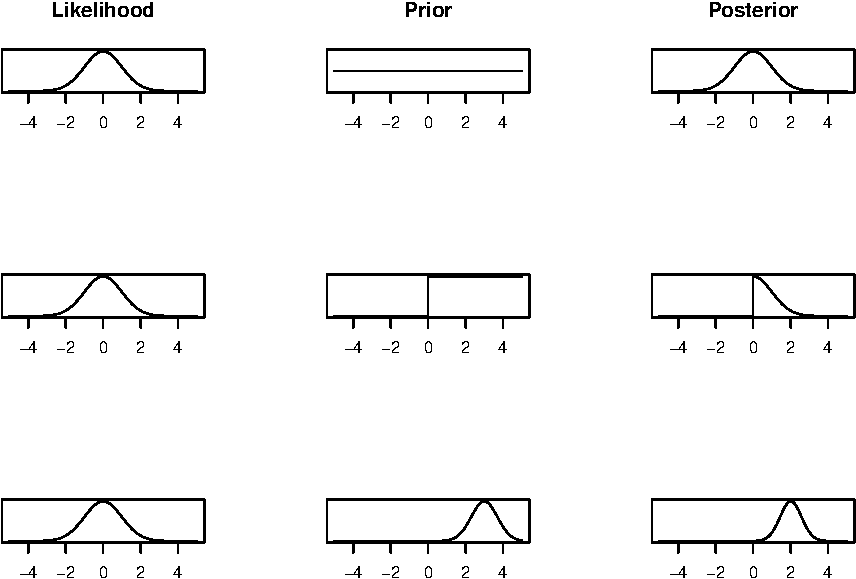
\includegraphics{_main_files/figure-latex/prior-posterior-grid-1.pdf}

\begin{enumerate}
\def\labelenumi{\arabic{enumi}.}
\item
  The posterior distribution is proportional to the likelihood function. The prior distribution closely matches frequentist inference. Both the MLE and posterior mean are 0.
\item
  We get a lopsided posterior distribution, that is proportional to the likelihood function for positive values of \(\theta\), but is 0 for negative values of \(\theta\).
\item
  We get some sort of average of the likelihood function and the prior distribution. Had we collected more data, the posterior distribution would have been weighted toward the information from the likelihood function more.
\end{enumerate}

\end{example}

\hypertarget{exercises}{%
\section{Exercises}\label{exercises}}

\begin{exercise}

Consider a standard pack of 52 playing cards. You pick a card at random, what is the probability you pick:

\begin{enumerate}
\def\labelenumi{\arabic{enumi}.}
\tightlist
\item
  A Queen, given you have picked a picture card (King, Queen, Jack)?
\item
  The five of clubs, given you have picked a black card?
\item
  A black card, given you have not picked the five of clubs?
\end{enumerate}

\end{exercise}

\begin{solution}

A pack of playing cards is equally divided into four suits: Hearts (red), Diamonds (red), Clubs (black), and Spades (black). Each suit has 13 cards numbered 2 - 10, Jack, Queen, King (all three picture cards), and Ace.

\begin{enumerate}
\def\labelenumi{\arabic{enumi}.}
\tightlist
\item
  \begin{align*}
  P(\hbox{Queen} \mid \hbox{Picture}) &= \frac{P(\hbox{Queen and Picture})}{P(\hbox{Picture)}} \\
  & = \frac{4/52}{12/52} \\
  & = \frac{1}{3}.
  \end{align*}
\item
  \begin{align*}
  P(\hbox{5 Clubs} \mid \hbox{Black}) &= \frac{P(\hbox{5 Clubs and Black})}{P(\hbox{Black)}} \\
  & = \frac{1/52}{1/2} \\
  & = \frac{1}{26}.
  \end{align*}
\item
  \begin{align*}
  P(\hbox{Black} \mid \hbox{Not 5 Clubs}) & = \frac{P(\hbox{Black} \mid \hbox{Not 5 Clubs})}{P(\hbox{Not 5 Clubs})} \\
  & = \frac{25/52}{51/52}\\
  &= \frac{25}{51}.
  \end{align*}
\end{enumerate}

\end{solution}

\begin{exercise}

Decide if each of the following events can be assigned probabilities by frequentists:

\begin{enumerate}
\def\labelenumi{\arabic{enumi}.}
\tightlist
\item
  The Bermuda triangle exists.
\item
  Getting a 6 when rolling a dice.
\item
  Someone will test positive for Covid-19 after contracting the disease.
\item
  The sun will rise tomorrow.
\end{enumerate}

\end{exercise}

\begin{solution}

\begin{enumerate}
\def\labelenumi{\arabic{enumi}.}
\tightlist
\item
  No, this can't be assigned a probability.
\item
  Yes, you can repeatedly roll of dice.
\item
  Yes, this can be assigned a probability. You can repeatedly test someone for the disease, hence there is a long-run frequency of the test returning a positive result.
\item
  It depends what you mean by tomorrow. Suppose today is 1st January 2023, if tomorrow means 2nd January 2023, then no. 2nd January 2023 will on occur once and there is no long-run frequency. If, however, you define tomorrow by the day after today, then yes. There have been many (The Earth has been going round the Sun for \textasciitilde4.5 billion years, so approximately 4.5*365 tomorrows), so it can be assigned a probability.
\end{enumerate}

\end{solution}

\begin{exercise}

An urn contains three coins. Two of the coins are fair, but one of the coins has heads on both sides.

\begin{enumerate}
\def\labelenumi{\arabic{enumi}.}
\tightlist
\item
  You pick a coin out of the urn without looking and flip it. What's the probability you get heads?
\item
  You pick a coin out of the urn without looking and flip it and get heads. What's the probability it's the two-headed coin?
\end{enumerate}

\end{exercise}

\begin{solution}

Label the coins 1, 2, 3, where \(P(\hbox{Heads} \mid \hbox{Coin } 1) = P(\hbox{Heads} \mid \hbox{Coin } 2) = \frac{1}{2}\) and \(P(\hbox{Heads} \mid \hbox{Coin } 3) = 1\).

\begin{enumerate}
\def\labelenumi{\arabic{enumi}.}
\item
  Using the law of total probability
  \begin{align*}
  P(\hbox{Heads}) & = P(\hbox{Heads} \mid \hbox{Coin } 1) P(\hbox{Coin } 1) + \\
  & \qquad  P(\hbox{Heads} \mid \hbox{Coin } 2) P(\hbox{Coin } 2) + P(\hbox{Heads} \mid \hbox{Coin } 3) P(\hbox{Coin } 3) \\
  & = \frac{1}{2}\cdot\frac{1}{3} + \frac{1}{2}\cdot\frac{1}{3} + 1\cdot\frac{1}{3} \\
  & = \frac{2}{3}.
  \end{align*}
\item
  Using Bayes' theorem
  \begin{align*}
  P(\hbox{Coin 1}\mid \hbox{Heads}) &= \frac{P(\hbox{Heads} \mid \hbox{Coin 1})P(\hbox{Coin 1})}{P(\hbox{Heads})} \\
  & = \frac{1\cdot\frac{1}{3}}{\frac{2}{3}} \\
  & = \frac{1}{2}.
  \end{align*}
\end{enumerate}

\end{solution}

\begin{exercise}

You see a sponsored post online with the word \emph{bitcoin} in. You want to work out the probability the post is spam.

\begin{enumerate}
\def\labelenumi{\arabic{enumi}.}
\tightlist
\item
  Using the law of total probability, show the probability the post is spam, given it contains the word probability is
  \[
    \pi(\textrm{spam} \mid \textrm{bitcoin}) = \frac{\pi(\textrm{bitcoin} \mid \textrm{spam})\pi(\textrm{spam})}{\pi(\textrm{bitcoin} \mid \textrm{spam})\pi(\textrm{spam}) + \pi(\textrm{bitcoin} \mid \textrm{not spam})\pi(\textrm{not spam})}
    \]
\item
  Most spam filters take a naive approach and set
  \[
    \pi(\textrm{spam}) =\pi(\textrm{not spam}) = \frac{1}{2}. 
    \]
  If an post is known to be spam, there's an 80\% chance it contains the word bitcoin. If an post is not spam, then there's a 1\% chance it contains the word bitcoin. Calculate the probability the post is spam given it contains bitcoin.
\item
  Suppose you take a much more pessimistic view, and assume that 80\% of all sponsered posts are spam. Recalculate the probability the post is spam given it contains bitcoin.
\end{enumerate}

\end{exercise}

\begin{solution}

By Bayes' theorem, we have
\[
 \pi(\textrm{spam} \mid \textrm{bitcoin}) = \frac{\pi(\textrm{bitcoin} \mid \textrm{spam})\pi(\textrm{spam})}{\pi(\textrm{bitcoin})}.
\]
1. By the law of total probability,
\[
\pi(\textrm{bitcoin}) = \pi(\textrm{bitcoin} \mid \textrm{spam})\pi(\textrm{spam}) + \pi(\textrm{bitcoin} \mid \textrm{not spam})\pi(\textrm{not spam}). 
\]
Thus,
\[
  \pi(\textrm{spam} \mid \textrm{bitcoin}) = \frac{\pi(\textrm{bitcoin} \mid \textrm{spam})\pi(\textrm{spam})}{\pi(\textrm{bitcoin} \mid \textrm{spam})\pi(\textrm{spam}) + \pi(\textrm{bitcoin} \mid \textrm{not spam})\pi(\textrm{not spam})}
\]

\begin{enumerate}
\def\labelenumi{\arabic{enumi}.}
\setcounter{enumi}{1}
\tightlist
\item
  From the question, we have \(\pi(\textrm{spam}) =\pi(\textrm{not spam}) = \frac{1}{2}\), \(\pi(\textrm{bitcoin} \mid \textrm{spam}) = 0.8\) and \(\pi(\textrm{bitcoin} \mid \textrm{not spam}) = 0.01\). Plugging these into the probability gives
  \[
    \pi(\textrm{spam} \mid \textrm{bitcoin}) = \frac{80}{81} \approx 98.7\%.
  \]
\item
  This time \(\pi(\textrm{spam}) = 0.8\) and \(\pi(\textrm{not spam}) = 0.2\), which yields
  \[
    \pi(\textrm{spam} \mid \textrm{bitcoin}) = \frac{320}{321} \approx 99.7\%.
  \]
\end{enumerate}

\end{solution}

\begin{exercise}

You are working on a project investigating pollution related illnesses in the West Midlands. I have sampled the proportion of people with pollution related illnesses in five areas of the West Midlands, \(y_1, \ldots, y_5\), with nothing to distinguish the data. This exercise is about the last data point \(y_5\).

\begin{enumerate}
\def\labelenumi{\arabic{enumi}.}
\tightlist
\item
  Should you model these data points exchangeably?
\item
  I now tell you the first four of these rates (0.72, 1.00, 0.85, 0.78 per 100,000). Should you continue to model these data points exchangeably?
\item
  Now, suppose instead of telling you these four rates, I had told you the five areas I have information about are Birmingham City Centre, Smethwick, Edgbaston, Dorridge, and Sutton Coldfield. Should you continue to model these data points exchangeably?
\item
  Now suppose I give you the data in part 2 and say that the missing data point \(y_5\) is Birmingham City Centre. Should you continue to model these data points exchangeably?
\end{enumerate}

\end{exercise}

\begin{solution}

This is based on Gelman et. al (2013, p.~105).

\begin{enumerate}
\def\labelenumi{\arabic{enumi}.}
\tightlist
\item
  Yes, you have no information to distinguish the data points so exchangability seems a reasonable assumption.
\item
  Yes, you still have no information to distinguish between any of the data points.
\item
  Yes, the joint distribution of these variables doesn't depend on the labels. However, you may start to formulate prior beliefs. Birmingham City Centre and Smethwick are likely to have higher rates of air pollution than leafy Dorridge.
\item
  No, these can no longer be modelled exchangably. You have reason to believe that Birmingham City Centre is likely to have a substantially higher value than the rest. That is you have information about \(\pi(y_5 > \max(y_1, y_2, y_3, y_4) \mid y_1, y_2, y_3, y_4)\), so exchangability is no longer a suitable assumption.
\end{enumerate}

\end{solution}

\hypertarget{programming-in-r}{%
\chapter{Programming in R}\label{programming-in-r}}

\hypertarget{random-numbers-for-loops-and-r}{%
\section{Random Numbers, For Loops and R}\label{random-numbers-for-loops-and-r}}

This first computer lab is about getting used to R. The first step is to download R and Rstudio.

\begin{itemize}
\tightlist
\item
  \href{https://www.r-project.org}{Download R}
\item
  \href{https://posit.co/downloads/}{Download RStudio IDE}
\end{itemize}

The easiest way to learn R is by using it to solve problems. The lab contains four exercises and three ways of approaching the exercise (easy, medium and hard). If you're new to R, use the easy approach and copy and paste the code straight into R -- you'll need to fill in a few blanks though. If you've used R before, or a similar programming language, stick to the medium and hard approaches. This is also an exercise in using Google. Googling around a problem of for specific commands can allow you to quickly find examples (most likely on Stack Overflow) with code you can use.

There are three aims of this lab:

\begin{enumerate}
\def\labelenumi{\arabic{enumi}.}
\tightlist
\item
  Getting used to programming in R.
\item
  Generating random numbers in R.
\item
  \href{https://www.w3schools.com/r/r_for_loop.asp}{Creating for loops in R}.
\end{enumerate}

\begin{example}
Computationally verify that the Poisson distribution with rate \(\lambda = 100\) can be approximated by a normal distribution with mean and variance 100.

To do this, we can generate lots of samples from a Poisson(100) distribution and plot them on top of the density function of the normal distribution with mean and variance 100.

R has four built-in functions for working with distributions. They take the form \texttt{rdist}, \texttt{ddist}, \texttt{pdist}, and \texttt{qdist}. You replace the \texttt{dist} part with the name of the distribution you want to work with, for example \texttt{unif} for the uniform distribution or \texttt{norm} for the normal distribution. As we are working with the the Poisson distribution, we will use \texttt{pois}. The prefixes allow you to work with the distribution in different ways: \texttt{r} gives you random numbers sampled form the distribution, \texttt{d} evaluates the density function, \texttt{p} evaluates the density function, and \texttt{q} evaluates the inverse density function (or quantile function).

The function \texttt{rpois} allows us to generate samples from a Poisson distribution. We store 10,000 samples in a vector \texttt{y} by calling

\begin{Shaded}
\begin{Highlighting}[]
\NormalTok{y }\OtherTok{\textless{}{-}} \FunctionTok{rpois}\NormalTok{(}\AttributeTok{n =} \DecValTok{10000}\NormalTok{, }\AttributeTok{lambda =} \DecValTok{100}\NormalTok{)}
\end{Highlighting}
\end{Shaded}

We can generate a histogram of \texttt{y} using the \texttt{hist} command. Setting \texttt{freq\ =\ FALSE}, makes R plot a density histogram instead of a frequency histogram. Typing \texttt{?hist} will give you more information about this

\begin{Shaded}
\begin{Highlighting}[]
\FunctionTok{hist}\NormalTok{(y, }\AttributeTok{freq =} \ConstantTok{FALSE}\NormalTok{, }\AttributeTok{xlab =} \StringTok{"y"}\NormalTok{, }\AttributeTok{main =} \StringTok{""}\NormalTok{)}
\end{Highlighting}
\end{Shaded}

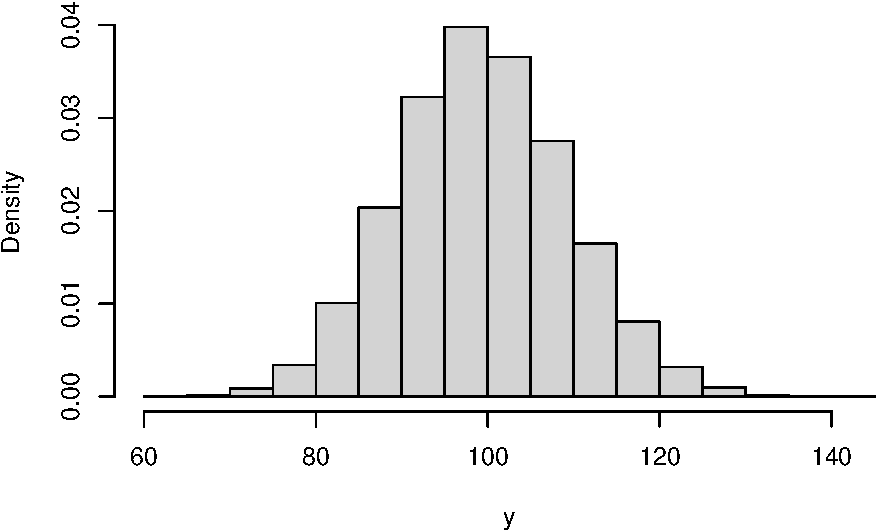
\includegraphics{_main_files/figure-latex/unnamed-chunk-3-1.pdf}

The last thing to do is to plot the normal density on top. There are a couple of ways of doing this. The way below generates a uniform grid of points and then evaluates the density at each point. Finally, it adds a line graph of these densities on top.

\begin{Shaded}
\begin{Highlighting}[]
\NormalTok{x }\OtherTok{\textless{}{-}} \FunctionTok{seq}\NormalTok{(}\AttributeTok{from =} \DecValTok{50}\NormalTok{, }\AttributeTok{to =} \DecValTok{150}\NormalTok{, }\AttributeTok{by =} \DecValTok{1}\NormalTok{)           }\CommentTok{\#create uniform grid on [50, 150]}
\NormalTok{density }\OtherTok{\textless{}{-}} \FunctionTok{dnorm}\NormalTok{(x, }\AttributeTok{mean =} \DecValTok{100}\NormalTok{, }\AttributeTok{sd =} \FunctionTok{sqrt}\NormalTok{(}\DecValTok{100}\NormalTok{)) }\CommentTok{\#compute density}

\CommentTok{\#plot together}
\FunctionTok{hist}\NormalTok{(y, }\AttributeTok{freq =} \ConstantTok{FALSE}\NormalTok{, }\AttributeTok{xlab =} \StringTok{"y"}\NormalTok{, }\AttributeTok{main =} \StringTok{""}\NormalTok{)}
\FunctionTok{lines}\NormalTok{(x, density)}
\end{Highlighting}
\end{Shaded}

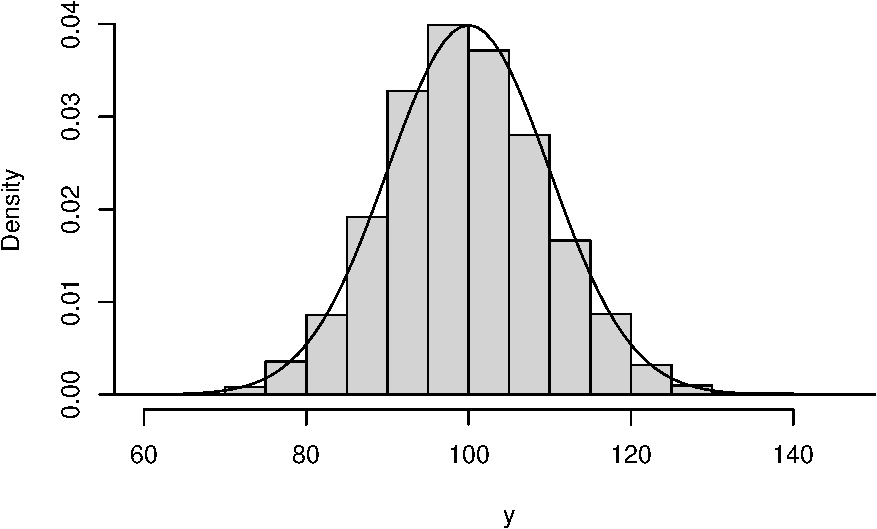
\includegraphics{_main_files/figure-latex/unnamed-chunk-4-1.pdf}

The two match up well, showing the normal distribution is a suitable approximation here.
\end{example}

Over the next two sessions, you will need to solve the following four problems in R. You can type \texttt{?} before any function in R (e.g.~\texttt{?rnorm}) to bring up R's helpage on the function. Googling can also bring up lots of information, possible solutions and support.

\begin{exercise}

The changes in the Birmingham stock exchange each day can be modelled using a normal distribution. The price on day \(i\), \(X_i\) is given by
\[
X_i = \alpha X_{i-1}, \qquad \alpha \sim N(1.001, 0.005^2).
\]
The index begins at \(X_0 = 100\). Investigate the distribution of the value of the stock market on days 50 and 100.

\textbf{Hard}. Use a simulation method to generate the relevant distributions.

\textbf{Medium}. Simulate the value for \(\alpha\) for each of the 100 days and use the \texttt{cumprod} command to plot a trajectory. Use a for loop to repeat this 100 times and investigate the distribution of the value of the stock market on days 50 and 100.

\textbf{Easy}. Fill in the blanks in the following code.

\begin{verbatim}
# Plot one ----------------------------------------------------------------
x <- rnorm(n = , mean = , sd = ) #Simulate daily change for 100 days
plot(, type = 'l') #multiply each day by the previous days

# Plot 100 realisations ---------------------------------------------------
market.index <- matrix(NA, 100, 100) #Initialise a matrix to store trajectories
for(i in 1:100){
  x <- rnorm(n = , mean = , sd = )
  market.index [, i] <- 
}

#Plot all trajectories
matplot(market.index, type = 'l')

#Get distribution of days 50 and 100
hist()
hist()
quantile(, )
quantile(, )
\end{verbatim}

\end{exercise}

\begin{exercise}

You are an avid lottery player and play the lottery twice a week, every week for 50 years (a total of 5,200 times). The lottery has 50 balls labeled 1, \ldots, 50 and you play the same 6 numbers each time. Six out of the 50 balls are chosen uniformly at random and the prize money is shown in the table below.

\begin{longtable}[]{@{}ll@{}}
\toprule()
Numbers Matched & Prize Amount \\
\midrule()
\endhead
0-2 & £0 \\
3 & £30 \\
4 & £140 \\
5 & £1,750 \\
6 & £1,000,000 \\
\bottomrule()
\end{longtable}

It costs you £2 to play each time. Simulate one set of 5,200 draws. How much do you win? What is your total profit/loss?

\textbf{Hard}. Use a for loop and sequence of if else statements to generate your prize winnings.

\textbf{Medium}. Use a for loop to generate the lottery numbers and prize winnings for each draw. Use the \texttt{sample} function to generate a set of lottery numbers and check they match against your numbers using the \texttt{\%in\%} function. Finally, use if else statements to check how much you have won each time.

\textbf{Easy}. Fill in the blanks in the following code.

\begin{verbatim}
my.numbers <- 

#For loop to generate lottery numbers and prize winnings
prize <- numeric(5200)
for(i in 1:5200){
  
  #Generate lottery numbers
  draw <- sample(, )
  
  #Check how many match my numbers
  numbers.matched <- #use %in% function
  
  #Compute prize winings
  if(numbers.matched < 3)
    prize[i] <- 0
  else if()
    prize[i] <-  30
  else if()
    prize[i] <-  140
  else if()
    prize[i] <-  1750
  else
    prize[i] <- 1000000
}

#Summarise prize winnings
table(prize)
hist(prize)
sum(prize) - 2*5200
\end{verbatim}

\end{exercise}

\begin{exercise}
Estimate \(\pi\).

\textbf{Hard}. Use a rejection sampling algorithm.

\textbf{Medium}. Generate lots of points \((x, y)\) on the unit square \([0, 1]^2\). Check each point to see if it lies within the unit circle. Use the proportion of points that lie within the unit circle to estimate \(\pi\).

\textbf{Easy}. Fill in the blanks in the following code.

\begin{verbatim}
#Sample on unit square
N <- 10000      #number of points
x <-            #sample N points uniformly at random on [0, 1]
y <-            #sample N points uniformly at random on [0, 1]

#Estimate pi
r.sq                 <- x^2 + y^2                #check how far from origin
number.inside.circle <-           #count how many points inside unit cirlce
pi.estimate          <- 

#Plot points
par(pty = "s")         #make sure plot is square
plot(x, y, cex = 0.1)  #plot points
theta <- seq(0, pi/2, 0.01) #plot unit circle
lines(x = cos(theta), y = sin(theta), col = "red")
\end{verbatim}

\textbf{Extra}. Use a for loop to repeat this for \(N = \{1, \ldots, 10000\}\). Record the estimate for \(\pi\) for each value and the relative error.
\end{exercise}

\begin{exercise}

A linear congruential generator (LCG) is a simple algorithm for generating random integers. Given a starting value \(X_0\), it generates a sequence of integers according to
\[
X_{i+1} = a X_i + c \mod m.
\]
Software that generates numbers using an LCG Setting \(a = 3\), \(c = 2\), \(m = 7\) and \(X_0 = 0\), generate 20 samples from this generator.

\begin{enumerate}
\def\labelenumi{\arabic{enumi}.}
\item
  Investigate the `randomness' of this generator by creating the delay plot, where \(X_{i-1}\) is plotted against \(X_{i}\)
\item
  One way to improve the quality of these generators is to shuffle the sequence generated. Generate rate two sequences \(X\) and \(Y\) from two different LCGs, and report the shuffled sequence \(Z_j = X_{Y_j}\). For the sequence \(Y\) use the values \(a = 5\), \(c = 1\), \(m = 8\) and \(Y_0 = 2\).
\item
  As the past two exercises show, LCGs are notoriously poor. in the 1960s and 70s, RANDU was a widely used LCG developed by IBM. According to Wikipedia
  \textgreater{} IBM's RANDU is widely considered to be one of the most ill-conceived random number generators ever designed, and was described as ``truly horrible'' by Donald Knuth.
\end{enumerate}

The RANDU LCG uses \(a = 2^{16} + 3\), \(c = 0\), \(m = 2^{31}\) and \(Y_0 = 1\). Generate a sequence of 10,000 pseudorandom variables from the RANDU LCG and create the delay plot.

The delay plot seems to show little relationship between \(X_{i}\) and \(X_{i+1}\). The third order delay plot is a 3d-plot with coordinate \((X_i, X_{i+1}, X_{i+2})\) and this plot shows a different picture. Create this plot using the code

\begin{verbatim}
#install.packages("scatterplot3d") #you may need to install this package
scatterplot3d::scatterplot3d(X[1:9998], X[2:9999], X[3:10000], angle=154, 
                             xlab = expression(X[i]), ylab = expression(X[i+1]), zlab = expression(X[i+2]))
\end{verbatim}

This is what makes the RANDU LCG so poor. Write down \(X_{i+1}\) and \(X_{i+2}\) in terms of \(X_i\). Show that \(X_{i+2} = \alpha X_{i+1} + \beta X_{i}\).

\textbf{Hard}. Use a for loop to construct sequences from the LCGs \(X\) and \(Y\).

\textbf{Medium}. Create a for loop to generate the value for the sequence \(X_i\) for \(i = 1, \ldots, 20\). Modular arithmetic can be performed using the \texttt{\%\%} function. Create a new for loop to construct the sequence \(Y\). To shuffle the sequence \(X\) using \(Y\), you will need to subset \(X\) by \(Y\) in R.

\textbf{Easy}. Fill in the blanks in the code below

\begin{verbatim}
# 1. Shuffling ---------------------------------------------------------------
X <- numeric(21) #initialise vector to store X

#Set values for LCG
a <- 
c <- 
m <- 
X[1]<- 


#Run Generator
for(i in 2:21){
  X[i] <-
}
X

#Delay plot
plot( , , xlab = expression(X[i-1]), ylab = expression(X[i]), type = 'l')



# 2. Shuffling ---------------------------------------------------------------

Y <- numeric(21) #initialise vector to store Y

#Set values for LCG
a <- 
c <- 
m <- 
Y[1]<- 


#Run Generator
for(i in 2:50){
  Y[i] <- 
}

#report sequence
Y
X[Y]

#Plot delay plot
plot(x = ,y = , xlab = expression(Z[i-1]), ylab = expression(Z[i]), type = 'l')
\end{verbatim}

\end{exercise}

\hypertarget{functions-in-r}{%
\section{Functions in R}\label{functions-in-r}}

The purpose of this lab is to learn how to write functions is R. Functions are wrappers that allow you to easily repeat commands, as well as customise specific pieces of code.

\hypertarget{built-in-commands}{%
\subsection{Built in commands}\label{built-in-commands}}

R has many build in commands and you used these in Computer Lab I. An example is the \texttt{runif} command from the second exercise. This function generates random numbers from an interval. The code chunk below shows it in action:

\begin{Shaded}
\begin{Highlighting}[]
\NormalTok{u }\OtherTok{\textless{}{-}} \FunctionTok{runif}\NormalTok{(}\AttributeTok{n =} \DecValTok{10}\NormalTok{, }\AttributeTok{min =} \SpecialCharTok{{-}}\DecValTok{1}\NormalTok{, }\AttributeTok{max =} \DecValTok{1}\NormalTok{)}
\NormalTok{u}
\end{Highlighting}
\end{Shaded}

\begin{verbatim}
##  [1]  0.09357866  0.62952178  0.99912039 -0.57849704  0.37552161  0.32493536
##  [7]  0.60381753  0.03332988 -0.13922159 -0.63415921
\end{verbatim}

The functions has three \textbf{arguments}: \emph{n} the number of samples to be generated, \emph{min} the lower limit of the interval, \emph{max} the upper limit of the interval. In the code chunk above 10 random numbers were generated from the interval {[}-1, 1{]}. In R, you don't need to label the arguments, so the following will sample the same number of samples from the same interval:

\begin{verbatim}
u <- runif(10, -1, 1)
\end{verbatim}

Although in most cases it helps to label the arguments for readability and avoiding undefined behaviour. Note that if you decide to omit the argument names in the function call, the arguments must appear exactly in the order defined by the function prototype (check the documentation ?function for specific cases).

\hypertarget{user-defined-functions}{%
\subsection{User defined functions}\label{user-defined-functions}}

In many cases, we will need to repeat the same piece of code over and over again, or we will need to run it again with different values. In this case, we can write our own function. In R, there are two ways to type your own function. The first is to write a full function definition. The basic template is

\begin{verbatim}
name.of.function <- function(arguments){

  #do something
  #produce result
  
  return(result)

}
\end{verbatim}

The second way is an in-line function, which is sometimes useful for short functions. The template is

\begin{verbatim}
name.of.function <- function(arguments) #do something
\end{verbatim}

In this module, we're going to use the full function way of writing functions.

\begin{example}
In this example, we're going to write a function to evaluate the normal density function. The density function is given by
\[
\pi(x \mid \mu, \sigma^2) = \frac{1}{\sqrt{2\pi\sigma^2}}e^{\left\{-\frac{1}{2\sigma^2}(x-\mu)^2\right\}}.
\]

We will need our function to take three arguments, the value at which the density function needs to be evaluated, and the mean and standard deviation of the distribution.

\begin{Shaded}
\begin{Highlighting}[]
\NormalTok{normal.density }\OtherTok{\textless{}{-}} \ControlFlowTok{function}\NormalTok{(x, mu, sigma)\{}
  
\NormalTok{  fraction.term }\OtherTok{\textless{}{-}} \DecValTok{1}\SpecialCharTok{/}\FunctionTok{sqrt}\NormalTok{(}\DecValTok{2}\SpecialCharTok{*}\NormalTok{pi}\SpecialCharTok{*}\NormalTok{sigma}\SpecialCharTok{\^{}}\DecValTok{2}\NormalTok{)}
\NormalTok{  exponent.term }\OtherTok{\textless{}{-}} \SpecialCharTok{{-}}\DecValTok{1}\SpecialCharTok{/}\NormalTok{(}\DecValTok{2}\SpecialCharTok{*}\NormalTok{sigma}\SpecialCharTok{\^{}}\DecValTok{2}\NormalTok{)}\SpecialCharTok{*}\NormalTok{(x}\SpecialCharTok{{-}}\NormalTok{mu)}\SpecialCharTok{\^{}}\DecValTok{2}
  
\NormalTok{  result }\OtherTok{\textless{}{-}}\NormalTok{ fraction.term}\SpecialCharTok{*}\FunctionTok{exp}\NormalTok{(exponent.term)}
  \FunctionTok{return}\NormalTok{(result)}
  
\NormalTok{\}}
\end{Highlighting}
\end{Shaded}

We have split up the density into two parts to make it easier to code up and read. R has its own inbuilt normal density function \texttt{dnorm} and we can compare our function against R's. Although R's is faster and more reliable, we should get the same results.

\begin{Shaded}
\begin{Highlighting}[]
\FunctionTok{normal.density}\NormalTok{(}\AttributeTok{x =} \FloatTok{0.5}\NormalTok{, }\AttributeTok{mu =} \DecValTok{1}\NormalTok{, }\AttributeTok{sigma =} \FloatTok{0.5}\NormalTok{)}
\end{Highlighting}
\end{Shaded}

\begin{verbatim}
## [1] 0.4839414
\end{verbatim}

\begin{Shaded}
\begin{Highlighting}[]
\FunctionTok{dnorm}\NormalTok{(}\AttributeTok{x =} \FloatTok{0.5}\NormalTok{, }\AttributeTok{mean =} \DecValTok{1}\NormalTok{, }\AttributeTok{sd =} \FloatTok{0.5}\NormalTok{)}
\end{Highlighting}
\end{Shaded}

\begin{verbatim}
## [1] 0.4839414
\end{verbatim}

Why might R's function be faster and more reliable than ours?
\end{example}

\begin{exercise}
Consider the stock exchange problem in Exercise 2.1. Write a function that simulates 100 days of the stock exchange. Use the \texttt{replicate} function to call this function 10,000 times.
\end{exercise}

\begin{exercise}

In a game, players can buy loot boxes. Each box contains one item chosen at random from fifty loot items in the game. By simulating lots of players buying loots boxes, what is the expected number of boxes a player needs to buy in order to collect all fifty items.

\begin{enumerate}
\def\labelenumi{\arabic{enumi}.}
\item
  Write a function that buys a new box and, it the player doesn't own it already, adds it to the set of items the player doesn't own already.
\item
  Write another function using a while loop that simulates a player buying boxes until they own all the items.
\item
  Use a for loop to simulate 10,000 players buying boxes until they own all the items.
\item
  It turns out there are three types of items in the loot boxes. 25 items are common, 20 are rare, and 5 are epic. Players are twice as likely to get at common item than a rare item, and four times as likely to get a rare item than an epic item. Modify the function from part 1 to account for this and repeat the simulation.
\end{enumerate}

\end{exercise}

\hypertarget{good-coding-practices}{%
\section{Good Coding Practices}\label{good-coding-practices}}

In the past two labs, we've written code to solve different problems. In this lab, we're going to take a step back and think about what good R code does and doesn't look like.

\hypertarget{code-style}{%
\subsection{Code Style}\label{code-style}}

Code should be both efficient and easy to read. In most cases it's better to write code that's easy to read and less efficient, than highly efficient code that's difficult to read. Some basic principles to make code easy to read are:

\begin{enumerate}
\def\labelenumi{\arabic{enumi}.}
\tightlist
\item
  Write short functions names, e.g.~\texttt{buy.loot.box} is better than \texttt{player.buys.one.loot.boox} or \texttt{blb}.
\item
  Document and comment code. In R comments start with \texttt{\#}.
\item
  Multiple short functions are better than long functions that do multiple things.
\item
  Be consistent.
\end{enumerate}

\begin{example}
Review the \href{https://style.tidyverse.org/index.html}{tidyverse Style Guide}.
\end{example}

\begin{example}
Review \href{https://google.github.io/styleguide/Rguide.html}{Google's R Style Guide}.
\end{example}

One way to ensure code style is consistent and bug free is to carry out code reviews. These are common both in academia and industry. A code review is where someone else goes through your code line-by-line ensuring it conforms to the company style and doesn't have any bugs.

\begin{exercise}

The following code is for Exercises 2.1 about the stock exchange. Restyle the code so it is easy to read.

\begin{verbatim}
# Plot one ----------------------------------------------------------------
rnorm(100,1.001,0.5) -> x 
plot(100*cumprod(x),type ='l') 
# Plot 100 realisations ---------------------------------------------------
X <- matrix(NA, 100, 100) 
for(i in 1:100){
  x <- rnorm(100, 1.001, 0.005)
  X[,i] <- 100*cumprod(x)
}
matplot(X,type ='l')
hist(X[50,]);hist(X[100,]);quantile(X[50,], c(0.25, 0.5, 0.75));quantile(X[100,], c(0.25, 0.5, 0.75))
\end{verbatim}

\end{exercise}

\begin{exercise}

In pairs or groups, carry out a code review for one of your solutions to an exercise from a previous lab. Remember to

\begin{enumerate}
\def\labelenumi{\arabic{enumi}.}
\tightlist
\item
  Make sure the coding style is consistent.
\item
  Identify any bugs.
\item
  Be respectful and constructive in your feedback.
\end{enumerate}

\end{exercise}

\hypertarget{bayesian-inference}{%
\chapter{Bayesian Inference}\label{bayesian-inference}}

Whereas Chapter 1 dealt with the fundamentals of Bayesian inference and definitions, Chapter 3 is much more practical. We are going to be deriving posterior distributions and proving when it does and doesn't work.

\hypertarget{the-binomial-distribution}{%
\section{The Binomial Distribution}\label{the-binomial-distribution}}

The first example we're going to go through is with the Binomial distribution.

\begin{example}
\protect\hypertarget{exm:binom}{}\label{exm:binom}A social media company wants to determine how many of its users are bots. A software engineer collects a random sample of 200 accounts and finds that eight are bots. She uses a Bayesian method to estimate the probability of an account being a bot. She labels the accounts with a 1 if they are a bot and 0 if there is are a real person. The set of account labels is given by \(\boldsymbol{y} = \{y_1, \ldots, y_{200}\}\) and the probability an account is a bot is \(\theta\). By Bayes' theorem, we obtain the following,
\[
\pi(\theta \mid \boldsymbol{y}) \propto \pi(\boldsymbol{y}\mid \theta) \pi(\theta).
\]

\textbf{Likelihood function} \(\pi(\boldsymbol{y}\mid \theta)\). We observe 200 trials each with the same probability of success (denoted by \(\theta\)) and probability of failure (given by \(1-\theta\)). The Binomial distribution seems the most suitable way of modelling this. Therefore, the likelihood function is given by,
\[
\pi(\boldsymbol{y}\mid \theta) = \begin{pmatrix} 200 \\ 3 \end{pmatrix} \theta^3(1-\theta)^{197},
\]
assuming that any two accounts being a bot are independent of one another.

\textbf{Prior distribution} \(\pi(\theta)\). We now need to describe our prior beliefs about \(\theta\). We have no reason to suggest \(\theta\) takes any specific value, so we use a uniform prior distribution \(\theta \sim U[0, 1]\), where \(\pi(\theta) = 1\) for \(\theta \in [0, 1]\).

\textbf{Posterior distribution} \(\pi(\theta \mid \boldsymbol{y})\). We can now derive the posterior distribution up to proportionality
\[
\pi(\theta \mid \boldsymbol{y}) \propto \theta^3(1-\theta)^{197}. 
\]
This functional dependence on \(\theta\) identifies the \(\pi(\theta \mid \boldsymbol{y})\) is a Beta distribution. The PDF for the beta distribution with shape parameters \(\alpha\) and \(\beta\) is
\[
\pi(x \mid \alpha, \beta) = \frac{\Gamma(\alpha + \beta)}{\Gamma(\alpha)\Gamma(\beta)}x^{\alpha - 1}(1-x)^{\beta - 1}. 
\]
The posterior distribution is therefore \(\theta \mid \boldsymbol{y} \sim \textrm{Beta}(4, 198)\).
\end{example}

\hypertarget{reporting-conclsuions-from-bayesian-inference}{%
\section{Reporting Conclsuions from Bayesian Inference}\label{reporting-conclsuions-from-bayesian-inference}}

In the previous example, we derived the posterior distribution \(\theta \mid \boldsymbol{y} \sim \textrm{Beta}(4, 198)\). But often, we want to share more descriptive information about our beliefs given the observed data. In this example, the posterior mean given the data is \(\frac{4}{198} = \frac{2}{99}\). That is to say given the data, we expect that for every 99 accounts, two to be bots. The posterior mode for \(\theta\) is \(\frac{3}{200}\) or 1.5\%.

It is important to share the uncertainty about out beliefs. In a frequentist framework, this would be via a confidence interval. The Bayesian analogues is a credible interval.

\begin{definition}
A \textbf{credible interval} is a central interval of posterior probability which corresponds, in the case of a 100\((1-\alpha)\)\% interval, to the range of values that capture 100\((1-\alpha)\)\% of the posterior probability.
\end{definition}

\begin{example}
The 95\% credible interval for the Binomial example is given by

\begin{Shaded}
\begin{Highlighting}[]
\NormalTok{cred.int}\FloatTok{.95} \OtherTok{\textless{}{-}} \FunctionTok{qbeta}\NormalTok{(}\FunctionTok{c}\NormalTok{(}\FloatTok{0.025}\NormalTok{, }\FloatTok{0.975}\NormalTok{), }\DecValTok{4}\NormalTok{, }\DecValTok{198}\NormalTok{)}
\FunctionTok{round}\NormalTok{(cred.int}\FloatTok{.95}\NormalTok{, }\DecValTok{3}\NormalTok{)}
\end{Highlighting}
\end{Shaded}

\begin{verbatim}
## [1] 0.005 0.043
\end{verbatim}

This says that we believe there is a 95\% chance that the probability of an account being a bot lies between 0.005 and 0.043. This is a much more intuitive definition to the confidence interval, which says if we ran the experiment an infinite number of times and computed an infinite number of confidence intervals, 95\% of them would contain the true value of \(\theta\).
\end{example}

\hypertarget{the-exponential-distribution}{%
\section{The Exponential Distribution}\label{the-exponential-distribution}}

\begin{example}
\protect\hypertarget{exm:exponential}{}\label{exm:exponential}

An insurance company want to estimate the time until a claim is made on a specific policy. They describe the rate at which claims come in by \(\lambda\). The company provides a sample of 10 months at which a claim was made \(\boldsymbol{y} = \{14, 10, 6, 7, 13, 9, 12, 7, 9, 8\}\). By Bayes' theorem, the posterior distribution for \(\lambda\) is
\[
\pi(\lambda \mid \boldsymbol{y}) \propto \pi(\boldsymbol{y} \mid \lambda) \pi(\lambda).
\]

\textbf{Likelihood function} \(\pi(\boldsymbol{y} \mid \lambda)\). The exponential distribution is a good way of modelling lifetimes or the length of time until an event happens. Assuming all the claims are independent of one another, the likelihood function is given by
\begin{align*}
\pi(\boldsymbol{y} \mid \lambda) &= \prod_{i=1}^{10} \lambda e^{-\lambda y_i} \\
& = \lambda^{10}e^{-\lambda \sum_{i=1}^{10} y_i} \\
& = \lambda^{10} e^{-95\lambda}.
\end{align*}

\textbf{Prior distribution} \(\pi(\lambda)\). As we are modelling a rate parameter, we know it must be positive and continuous. We decide to use an exponential prior distribution for \(\lambda\), but leave the choice of the rate parameter up to the insurance professionals at the insurance company. The prior distribution is given by \(\lambda \sim \textrm{Exp}(\gamma).\)

\textbf{Posterior distribution} \(\pi(\lambda \mid \boldsymbol{y})\). We now have all the ingredients to derive the posterior distribution. It is given by
\begin{align*}
\pi(\lambda \mid \boldsymbol{y}) &\propto \lambda^{10} e^{-95\lambda} \times \lambda e^{-\gamma\lambda} \\
& \propto \lambda^{11}e^{-(95 + \gamma)\lambda}
\end{align*}
The functional form tells us that the posterior distribution is a Gamma distribution. The PDF of a gamma random variable with shape \(\alpha\) and rate \(\beta\) is
\[
\pi(x \mid \alpha, \beta) = \frac{\alpha^\beta}{\Gamma(\alpha)}x^{\alpha-1}e^{-\beta x}.
\]
The distribution of the rate of the claims given the observed data is \(\lambda \mid \boldsymbol{y} \sim \textrm{Gamma}(10, 95 + \gamma)\).

The posterior mean months until a claim is \(\frac{10}{95 + \gamma}\). We can see the effect of the choice of rate parameter in this mean. Small values of \(\gamma\) yield vague prior distribution, which plays a minimal role in the posterior distribution. Large values of \(\gamma\) result in prior distributions that contribute a lot to the posterior distribution. The plots below show the prior and posterior distributions for \(\gamma = 0.01\) and \(\gamma = 50\).

\begin{Shaded}
\begin{Highlighting}[]
\NormalTok{plot.distributions }\OtherTok{\textless{}{-}} \ControlFlowTok{function}\NormalTok{(chi)\{}
  \CommentTok{\#evaluate at selected values of theta}
\NormalTok{  theta }\OtherTok{\textless{}{-}} \FunctionTok{seq}\NormalTok{(}\FloatTok{0.001}\NormalTok{, }\FloatTok{0.3}\NormalTok{, }\FloatTok{0.001}\NormalTok{) }
  
  \CommentTok{\#evaluate prior density}
\NormalTok{  prior }\OtherTok{\textless{}{-}} \FunctionTok{dexp}\NormalTok{(theta, }\AttributeTok{rate =}\NormalTok{ chi)}
  
  \CommentTok{\#evaluate posterior density}
\NormalTok{  posterior }\OtherTok{\textless{}{-}} \FunctionTok{dgamma}\NormalTok{(theta, }\AttributeTok{shape =} \DecValTok{10}\NormalTok{, }\AttributeTok{rate =} \DecValTok{95} \SpecialCharTok{+}\NormalTok{ chi)}
  
  
  \CommentTok{\#plot}
  \FunctionTok{plot}\NormalTok{(theta, posterior, }\AttributeTok{type=} \StringTok{\textquotesingle{}l\textquotesingle{}}\NormalTok{, }
       \AttributeTok{ylim =} \FunctionTok{c}\NormalTok{(}\DecValTok{0}\NormalTok{, }\DecValTok{50}\NormalTok{), }\AttributeTok{xlab =} \FunctionTok{expression}\NormalTok{(theta), }\AttributeTok{ylab =} \StringTok{"density"}\NormalTok{)}
  \FunctionTok{lines}\NormalTok{(theta, prior, }\AttributeTok{lty =} \DecValTok{2}\NormalTok{)}
  \FunctionTok{legend}\NormalTok{(}\StringTok{\textquotesingle{}topright\textquotesingle{}}\NormalTok{, }\AttributeTok{lty =} \FunctionTok{c}\NormalTok{(}\DecValTok{1}\NormalTok{, }\DecValTok{2}\NormalTok{), }\AttributeTok{legend =} \FunctionTok{c}\NormalTok{(}\StringTok{"Posterior"}\NormalTok{, }\StringTok{"Prior"}\NormalTok{),  }
         \AttributeTok{bty =} \StringTok{"n"}\NormalTok{)}
\NormalTok{\}}

\FunctionTok{plot.distributions}\NormalTok{(}\FloatTok{0.01}\NormalTok{)}
\end{Highlighting}
\end{Shaded}

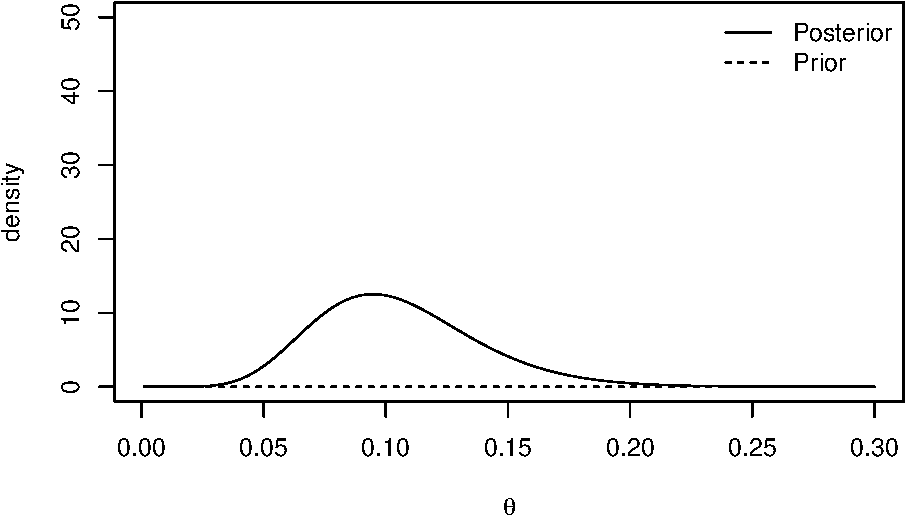
\includegraphics{_main_files/figure-latex/unnamed-chunk-9-1.pdf}

\begin{Shaded}
\begin{Highlighting}[]
\FunctionTok{plot.distributions}\NormalTok{(}\DecValTok{50}\NormalTok{)}
\end{Highlighting}
\end{Shaded}

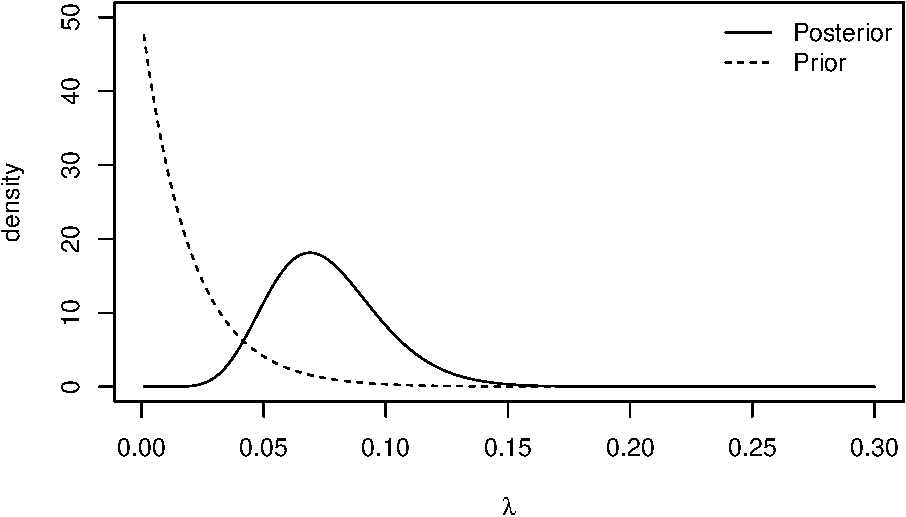
\includegraphics{_main_files/figure-latex/unnamed-chunk-9-2.pdf}

The insurance managers recommend that because this is a new premium, a vague prior distribution be used and \(\gamma = 0.01\). The posterior mean is \(\frac{10}{95.01} \approx 0.105\) and the 95\% credible interval is

\begin{Shaded}
\begin{Highlighting}[]
\FunctionTok{round}\NormalTok{(}\FunctionTok{qgamma}\NormalTok{(}\FunctionTok{c}\NormalTok{(}\FloatTok{0.025}\NormalTok{, }\FloatTok{0.975}\NormalTok{), }\DecValTok{10}\NormalTok{, }\FloatTok{95.01}\NormalTok{), }\DecValTok{3}\NormalTok{)}
\end{Highlighting}
\end{Shaded}

\begin{verbatim}
## [1] 0.05 0.18
\end{verbatim}

\end{example}

\hypertarget{the-normal-distribtuion}{%
\section{The Normal Distribtuion}\label{the-normal-distribtuion}}

The Normal distribution is incredibly useful for modelling a wide range of natural phenomena and in its own right. We're now going to derive posterior distributions for the normal distribution. As we're going to see, the concepts behind deriving posterior distributions are the same as in the previous two examples. However, the algebraic accounting is a lot more taxing.

\begin{example}
\protect\hypertarget{exm:normal}{}\label{exm:normal}

Reaction times can be modeled with a normal distribution. Suppose we have a data set of the reaction times of 30 lorry drivers when they see an obstacle. The reaction times were collected in a test environment on a rolling road. The time until each lorry driver reacts (in milliseconds) is

\begin{Shaded}
\begin{Highlighting}[]
\NormalTok{y }\OtherTok{\textless{}{-}} \FunctionTok{c}\NormalTok{(}\FloatTok{0.34}\NormalTok{, }\FloatTok{0.47}\NormalTok{, }\FloatTok{0.58}\NormalTok{, }\FloatTok{0.27}\NormalTok{, }\FloatTok{0.74}\NormalTok{, }\FloatTok{0.44}\NormalTok{, }\FloatTok{0.46}\NormalTok{, }\FloatTok{0.65}\NormalTok{, }\FloatTok{0.36}\NormalTok{, }\FloatTok{0.55}\NormalTok{, }\FloatTok{0.58}\NormalTok{, }\FloatTok{0.55}\NormalTok{, }\FloatTok{0.53}\NormalTok{, }\FloatTok{0.56}\NormalTok{, }\FloatTok{0.54}\NormalTok{, }\FloatTok{0.61}\NormalTok{, }\FloatTok{0.43}\NormalTok{, }\FloatTok{0.52}\NormalTok{, }\FloatTok{0.45}\NormalTok{, }\FloatTok{0.49}\NormalTok{, }\FloatTok{0.32}\NormalTok{, }\FloatTok{0.33}\NormalTok{, }\FloatTok{0.47}\NormalTok{, }\FloatTok{0.58}\NormalTok{, }\FloatTok{0.34}\NormalTok{, }\FloatTok{0.60}\NormalTok{, }\FloatTok{0.59}\NormalTok{, }\FloatTok{0.43}\NormalTok{, }\FloatTok{0.57}\NormalTok{, }\FloatTok{0.34}\NormalTok{)}
\FunctionTok{hist}\NormalTok{(y, }\AttributeTok{main =} \StringTok{""}\NormalTok{, }\AttributeTok{xlab =} \StringTok{"Reaction time (ms)"}\NormalTok{)}
\end{Highlighting}
\end{Shaded}

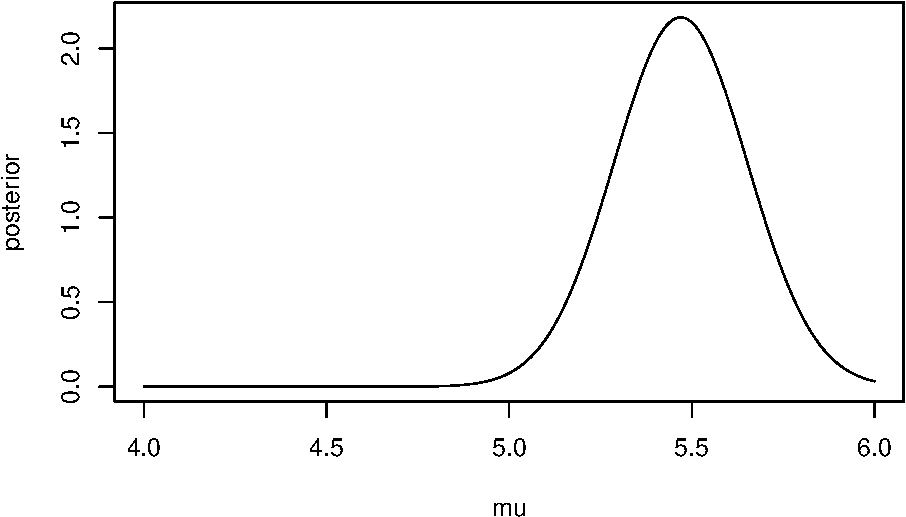
\includegraphics{_main_files/figure-latex/unnamed-chunk-11-1.pdf}

\begin{Shaded}
\begin{Highlighting}[]
\FunctionTok{mean}\NormalTok{(y)}
\end{Highlighting}
\end{Shaded}

\begin{verbatim}
## [1] 0.4896667
\end{verbatim}

Suppose that, somehow, we know the population standard deviation is 0.01\(ms\) and we wish to estimate the population mean \(\mu\). By Bayes' theorem, the posterior distribution is
\[
\pi(\mu \mid \boldsymbol{y}, \sigma^2) \propto \pi(\boldsymbol{y} \mid \mu, \sigma^2) \pi(\mu)
\]

\textbf{Likelihood function}. We assume the each driver's reaction time is independently and identically distributed such that
\[
y_i \sim N(\mu, \sigma^2)
\]
The likelihood function is therefore given by the product of the 30 normal density functions as follows,
\begin{align*}
\pi(\boldsymbol{y} \mid \mu, \theta^2) &= \prod_{i=1}^{30} \frac{1}{\sqrt{2\pi\sigma^2}}\exp\left\{-\frac{(y_i - \mu)^2}{2\sigma^2}\right\} \\
&= (2\pi\sigma^2)^{-\frac{30}{2}}\exp\left\{-\sum_{i=1}^{30}\frac{(y_i - \mu)^2}{2\sigma^2}\right\}.
\end{align*}

\textbf{Prior distribution} We suppose we have no prior beliefs about the values that \(\mu\) can take. We assign a normal prior distribution to \(\mu \sim N(\mu_0, \sigma_0^2)\) despite it being a time. We will set \(\mu = 0\) and \(\sigma_0^2 = 1000\) to signify our vague prior beliefs, but, for ease, we will use the symbolic values during the derivation of the posterior distribution. We have
\[
\pi(\mu) = \frac{1}{\sqrt{2\pi\sigma_0^2}}\exp\left\{-\frac{1}{2\sigma_0^2}(\mu - \mu_0)^2\right\}.
\]

\textbf{Posterior distribution}. To derive the posterior distribution, up to proportionality, we multiply the prior distribution by the likelihood function. As the fractions out the front of both terms do not depend on \(\mu\), we can ignore these.
\begin{align*}
\pi(\mu \mid \boldsymbol{y}, \sigma^2) &\propto\exp\left\{-\sum_{i=1}^{30}\frac{(y_i - \mu)^2}{2\sigma^2}\right\}  \exp\left\{\frac{1}{2\sigma_0^2}(\mu - \mu_0)^2\right\} \\
& = \exp\left\{-\sum_{i=1}^{30}\frac{(y_i - \mu)^2}{2\sigma^2}-\frac{1}{2\sigma_0^2}(\mu - \mu_0)^2\right\} \\
& = \exp\left\{-\frac{\sum_{i=1}^{30}y_i^2}{2\sigma^2} + \frac{\mu\sum_{i=1}^{30}y_i}{\sigma^2} - \frac{30\mu^2}{2\sigma^2} - \frac{\mu^2}{2\sigma_0^2} + \frac{\mu\mu_0}{\sigma_0^2} - \frac{\mu_0^2}{2\sigma_0^2}\right\}.
\end{align*}

We can drop the first and last term as they do not depend on \(\mu\). With some arranging, the equation becomes
\[
\pi(\mu \mid \boldsymbol{y}, \sigma^2) \propto \exp\left\{-\mu^2\left(\frac{30}{2\sigma^2}  + \frac{1}{2\sigma_0^2}\right) + \mu\left(\frac{\sum_{i=1}^{30}y_i}{\sigma^2} + \frac{\mu_0}{\sigma_0^2} \right)  \right\}
\]
Defining \(\mu_1 =\left(\frac{\sum_{i=1}^{30}y_i}{\sigma^2} + \frac{\mu_0}{\sigma_0^2} \right)\) and \(\sigma^2_1 = \left(\frac{30}{\sigma^2} + \frac{1}{\sigma_0^2}\right)^{-1}\) tidies this up and gives
\[
\pi(\mu \mid \boldsymbol{y}, \sigma^2) \propto \exp\left\{-\frac{\mu^2}{2\sigma_1^2} + \mu\mu_1 \right\}.
\]
Our last step to turning this into a distribution is completing the square. Consider the exponent term, completing the square becomes
\[
-2\sigma_1^2\mu^2 + \mu\mu_1 = -\frac{1}{2\sigma^2_1}\left(\mu - \frac{\mu_1}{\sigma_1^2} \right)^2.
\]
Therefore, the posterior distribution, up to proportionality, is given by
\[
\pi(\mu \mid \boldsymbol{y}, \sigma^2) \propto \exp\left\{-\frac{1}{2\sigma^2_1}\left(\mu - \frac{\mu_1}{\sigma_1^2} \right)^2\right\},
\]
and so the posterior distribution of \(\mu\) is \(\mu \mid \boldsymbol{y}, \sigma^2 \sim N(\mu_1, \sigma^2_1)\).

It may help to consider the meaning of \(\mu_1\) and \(\sigma^2_1\). The variance of the posterior distribution can be thought of as the weighted average of the population and sample precision, where the weight is the number of data points collected. The interpretation of the posterior mean can be seen more easily by writing is as
\[
\mu  = \sigma_1^2\left(\frac{30\bar{y}}{\sigma^2} + \frac{\mu_0}{\sigma_0^2} \right).
\]
The posterior mean is partially defined through the weighted average of the population and prior means, where the weighting depends on the number of data points collected and how precise the distributions are.

Now we have derived the posterior distribution, we can explore it using R.

\begin{Shaded}
\begin{Highlighting}[]
\CommentTok{\#data}
\NormalTok{N }\OtherTok{\textless{}{-}} \DecValTok{30}

\CommentTok{\#prior}
\NormalTok{sigma0 }\OtherTok{\textless{}{-}} \DecValTok{1000}
\NormalTok{mu0     }\OtherTok{\textless{}{-}} \DecValTok{0}

\CommentTok{\#posterior}
\NormalTok{sigma1.sq }\OtherTok{\textless{}{-}}\NormalTok{ (}\DecValTok{1}\SpecialCharTok{/}\NormalTok{(sigma0}\SpecialCharTok{\^{}}\DecValTok{2}\NormalTok{)  }\SpecialCharTok{+}\NormalTok{ N}\SpecialCharTok{/}\NormalTok{(}\FloatTok{0.01}\SpecialCharTok{\^{}}\DecValTok{2}\NormalTok{))}\SpecialCharTok{\^{}{-}}\DecValTok{1}
\NormalTok{mu1       }\OtherTok{\textless{}{-}}\NormalTok{ sigma1.sq}\SpecialCharTok{*}\NormalTok{(}\FunctionTok{sum}\NormalTok{(y)}\SpecialCharTok{/}\NormalTok{(}\FloatTok{0.01}\SpecialCharTok{\^{}}\DecValTok{2}\NormalTok{) }\SpecialCharTok{+}\NormalTok{ mu0}\SpecialCharTok{/}\NormalTok{(sigma0}\SpecialCharTok{\^{}}\DecValTok{2}\NormalTok{))}

\FunctionTok{c}\NormalTok{(mu1, sigma1.sq) }\CommentTok{\#output mean and variance}
\end{Highlighting}
\end{Shaded}

\begin{verbatim}
## [1] 4.896667e-01 3.333333e-06
\end{verbatim}

\begin{Shaded}
\begin{Highlighting}[]
\CommentTok{\#Create plot}
\NormalTok{mu }\OtherTok{\textless{}{-}} \FunctionTok{seq}\NormalTok{(}\FloatTok{0.48}\NormalTok{, }\FloatTok{0.5}\NormalTok{, }\FloatTok{0.0001}\NormalTok{) }
\NormalTok{posterior }\OtherTok{\textless{}{-}} \FunctionTok{dnorm}\NormalTok{(mu, }\AttributeTok{mean =}\NormalTok{ mu1, }\AttributeTok{sd =} \FunctionTok{sqrt}\NormalTok{(sigma1.sq))}
\FunctionTok{plot}\NormalTok{(mu, posterior, }\AttributeTok{type =}\StringTok{\textquotesingle{}l\textquotesingle{}}\NormalTok{)}
\end{Highlighting}
\end{Shaded}

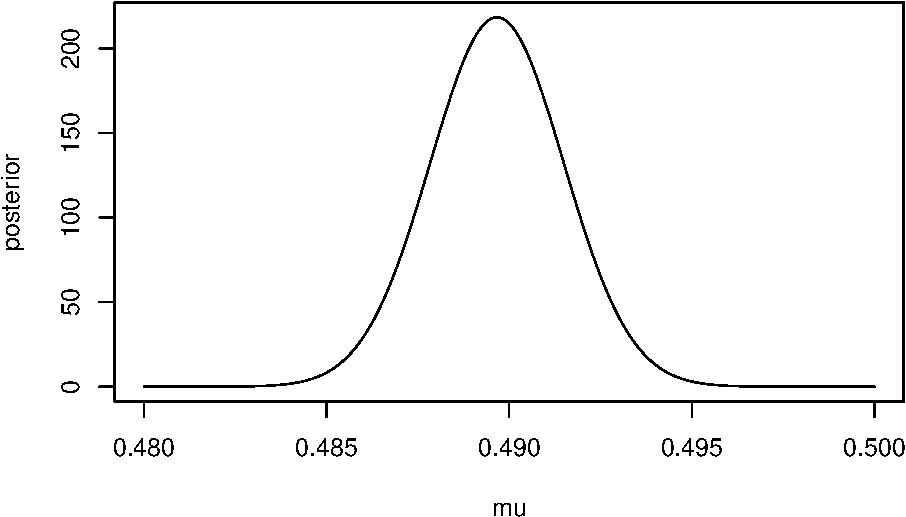
\includegraphics{_main_files/figure-latex/unnamed-chunk-12-1.pdf}

The 95\% credible interval for the population's mean reaction time is

\begin{Shaded}
\begin{Highlighting}[]
\FunctionTok{qnorm}\NormalTok{(}\FunctionTok{c}\NormalTok{(}\FloatTok{0.025}\NormalTok{, }\FloatTok{0.975}\NormalTok{), mu1, }\FunctionTok{sqrt}\NormalTok{(sigma1.sq))}
\end{Highlighting}
\end{Shaded}

\begin{verbatim}
## [1] 0.4860883 0.4932451
\end{verbatim}

\end{example}

One issue in this example is the choice of the prior distribution for \(\mu\). Why are we putting a prior distribution that places weight on negative values, when we are modelling reaction times? We could argue that the resulting posterior distribution places negligible weight on invalid times. The real reason is analytical ease. The resulting posterior distribution has a nice closed form, the normal distribution. When the prior distribution induces the same function form in the posterior distribution, this is known as conjugacy.

If the prior distribution \(\pi(\theta)\) has the same distributional family as the posterior distribution \(\pi(\theta \mid \boldsymbol{y})\), then the prior distribution is a \textbf{conjugate prior distribution}.

\hypertarget{hierarchical-models}{%
\section{Hierarchical Models}\label{hierarchical-models}}

In many modelling problems, there will be multiple parameters each related to one another. These parameters may be directly related to the model, or they may be parameters we introduce through prior distributions. We can form a hierarchy of these parameters, from closest to further from the data, to construct our model.

\begin{example}
Let's consider @ref\{exm:exponential\} again. We have some data \(\boldsymbol{y}\) that are assumed to have been generated from an Exponential distribution with rate parameter \(\lambda\). We placed an Exponential prior distribution with rate \(\gamma\) on \(\lambda\) and the posterior distribution was \(\lambda \mid \boldsymbol{y} \sim \textrm{Gamma}(10, 95 + \gamma)\).

In that example, we discussed how the choice of \(\gamma\) can affect the posterior distribution and conclusions presented to the company. One option is to place a prior distribution on \(\gamma\) -- a hyperprior distribution. The hierachy formed is
\begin{align*}
\boldsymbol{y} \mid \lambda &\sim \hbox{Exp}(\lambda) & \textrm{(likelihood)} \\
\lambda \mid \gamma &\sim \hbox{Exp}(\gamma) & \textrm{(prior distribution)} \\
\gamma \mid \nu &\sim \hbox{Exp}(\nu) & \textrm{(hyperprior distribution)}  \\
\end{align*}.

By Bayes' theorem, we can write the posterior distribution as
\begin{align*}
\pi(\lambda, \gamma \mid \boldsymbol{y}) &\propto \pi(\boldsymbol{y} \mid \lambda)\pi(\lambda \mid \gamma)\pi(\gamma)
&\propto \lambda^{11}e^{-\lambda(95 + \gamma)}\nu e^{-\nu\gamma}.
\end{align*}

To derive the full conditional distributions, we only consider the terms that depends on the parameters we are interested in. The full conditional distribution for \(\lambda\) is
\[
\pi(\lambda \mid \boldsymbol{y}, \,\gamma) \propto \lambda^{11}e^{-\lambda(95 + \gamma)}.
\]
This is unchanged and shows that \(\lambda \mid \boldsymbol{y}, \gamma \sim \textrm{Gamma}(10, 95 + \gamma)\). The full conditional distribution for \(\gamma\) is
\[
\pi(\gamma \mid \boldsymbol{y}, \,\lambda) \propto e^{-\nu\gamma}.
\]
Therefore the full conditional distribution of \(\gamma\) is \(\gamma \mid \boldsymbol{y}, \,\lambda \sim \hbox{Exp}(\lambda + \nu)\).
In the next chapter, we will look at how to sample from these distributions.
\end{example}

\hypertarget{prediction}{%
\section{Prediction}\label{prediction}}

In many cases, although we are interested in drawing inference for the model parameters, what we may also be interested in is predicting new values, whose distribution is determined by the model parameters and observed data.

\begin{definition}
Suppose we observe some data \(\boldsymbol{y}\) given some model parameters \(\theta\) and assign a prior distribution to \(\theta\) and hence derive the posterior distribution \(\pi(\theta \mid \boldsymbol{y})\). The quantity we are interested in is some future observation \(z\), we would like to the distribution of \(z\) given the observed data \(\boldsymbol{y}\), denoted by \(\pi(z \mid \boldsymbol{y})\). This distribution, known as the \textbf{posterior predictive distribution} of \(z\) must be exhibited as a mixture distribution over the possible values of \(\theta\) and is written as,
\[
\pi(z \mid \boldsymbol{y}) = \int \pi(z \mid \theta) \pi(\theta \mid \boldsymbol{y})\, d\theta.
\]
\end{definition}

\begin{example}

Students have to submit coursework for a particular statistical modules. However, each semester a number of students miss the deadline and hand in their coursework late. Last year, three out of 20 students handed their coursework in late. This year, the course has thirty students in. How many students can we expect to hand in their coursework late?

We can model the number of students handing their coursework in late, denoted by \(Y\), using a Binomial distribution, i.e.~\(Y \sim \textrm{Bin}(n, \theta)\) where \(n\) is the number of students and \(\theta\) is the probability of any particular student handing in their coursework late. As in Example \ref{exm:binom}, we assign a uniform prior distribution to \(\theta \sim U[0, 1]\). Given then observed data, we can derive \(\theta \mid \boldsymbol{y} \sim Beta(4, 28)\) (See problem sheets for derivation).

Now we can derive the posterior predictive distribution of \(Z\), the number of students who hand in late. We model \(Z\) using a Binomial distribution, \(Z \sim \textrm{Bin}(30, \theta)\). The distribution of \(Z\) given the observed data is

\begin{align*}
\pi(z \mid \boldsymbol{y}) &= \int_0^1 \pi(z \mid \theta) \pi(\theta \mid \boldsymbol{y})\, d\theta \\
& = \int_0^1 \begin{pmatrix} 30 \\ z \end{pmatrix} \theta^z (1-\theta)^{30 - z} \frac{\Gamma(32)}{\Gamma(4)\Gamma(28)}\theta^{3}(1-\theta)^{27}\, d\theta \\
 & = \begin{pmatrix} 30 \\ z \end{pmatrix}\frac{\Gamma(32)}{\Gamma(4)\Gamma(28)}\int_0^1 \theta^{z + 3}(1-\theta)^{57 - z}\, d\theta \\
\end{align*}
This integral is difficult to evaluate immediately. But by multiplying (and dividing outside the integral) by a constant, we can turn it into the density function of a Beta\((5 + z, 58 - z)\) random variable. This integrates to 1.

\begin{align*}
\pi(z \mid \boldsymbol{y})  & = \begin{pmatrix} 30 \\ z \end{pmatrix}\frac{\Gamma(32)}{\Gamma(4)\Gamma(28)}\frac{\Gamma(z+4)\Gamma(58-z)}{\Gamma(62)}\int_0^1 \frac{\Gamma(62)}{\Gamma(z+4)\Gamma(58-z)}\theta^{z + 3}(1-\theta)^{57 - z}\, d\theta \\ 
& = \begin{pmatrix} 30 \\ z \end{pmatrix}\frac{\Gamma(32)\Gamma(z+4)\Gamma(58-z)}{\Gamma(4)\Gamma(28)\Gamma(62)} \quad \textrm{for }  z \in \{0,1,...,30 \}.
\end{align*}

This code implements the distribution

\begin{Shaded}
\begin{Highlighting}[]
\NormalTok{beta.binom.posterior.predictive.distribution }\OtherTok{\textless{}{-}} \ControlFlowTok{function}\NormalTok{(z)\{}
  
  
\NormalTok{  numerator }\OtherTok{\textless{}{-}} \FunctionTok{gamma}\NormalTok{(}\DecValTok{32}\NormalTok{)}\SpecialCharTok{*}\FunctionTok{gamma}\NormalTok{(z }\SpecialCharTok{+} \DecValTok{4}\NormalTok{)}\SpecialCharTok{*}\FunctionTok{gamma}\NormalTok{(}\DecValTok{58}\SpecialCharTok{{-}}\NormalTok{z)}
\NormalTok{  denominator }\OtherTok{\textless{}{-}} \FunctionTok{gamma}\NormalTok{(}\DecValTok{4}\NormalTok{)}\SpecialCharTok{*}\FunctionTok{gamma}\NormalTok{(}\DecValTok{28}\NormalTok{)}\SpecialCharTok{*}\FunctionTok{gamma}\NormalTok{(}\DecValTok{62}\NormalTok{)}
  
\NormalTok{  output }\OtherTok{\textless{}{-}} \FunctionTok{choose}\NormalTok{(}\DecValTok{30}\NormalTok{, z)}\SpecialCharTok{*}\NormalTok{numerator}\SpecialCharTok{/}\NormalTok{denominator}
  \FunctionTok{return}\NormalTok{(output)}
  
\NormalTok{\}}
\end{Highlighting}
\end{Shaded}

We can check that our posterior predictive distribution is a valid probability mass function by checking that the probabilities sum to one.

\begin{Shaded}
\begin{Highlighting}[]
\NormalTok{z }\OtherTok{\textless{}{-}} \DecValTok{0}\SpecialCharTok{:}\DecValTok{30}
\NormalTok{ppd }\OtherTok{\textless{}{-}} \FunctionTok{beta.binom.posterior.predictive.distribution}\NormalTok{(z)}
\FunctionTok{sum}\NormalTok{(ppd)}
\end{Highlighting}
\end{Shaded}

\begin{verbatim}
## [1] 1
\end{verbatim}

\begin{Shaded}
\begin{Highlighting}[]
\FunctionTok{plot}\NormalTok{(z, ppd, }\AttributeTok{xlab =} \StringTok{"z"}\NormalTok{, }\AttributeTok{ylab =} \StringTok{"Posterior predictive mass"}\NormalTok{)}
\end{Highlighting}
\end{Shaded}

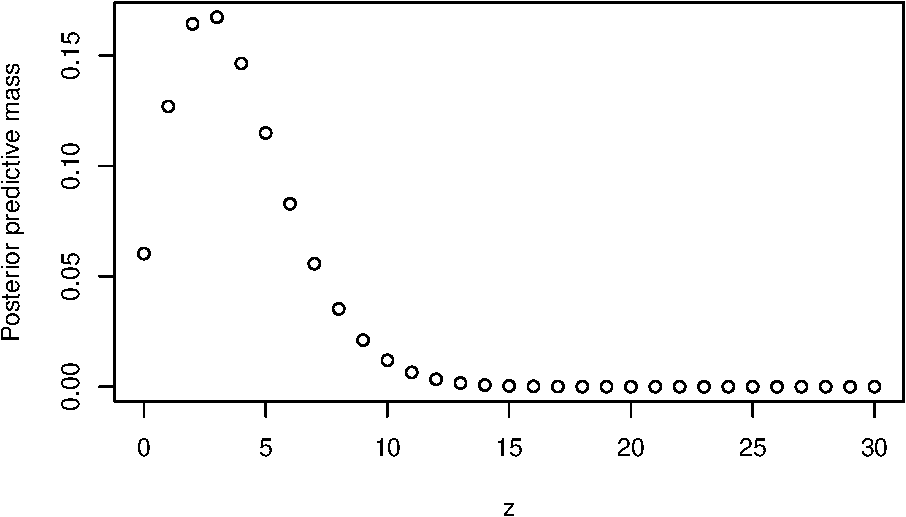
\includegraphics{_main_files/figure-latex/unnamed-chunk-15-1.pdf}

The expected number of students who hand in late is 3.75 and there's a 95\% chance that up to 8 hand in late.

\begin{Shaded}
\begin{Highlighting}[]
\NormalTok{z}\SpecialCharTok{\%*\%}\NormalTok{ppd }\CommentTok{\#expectation}
\end{Highlighting}
\end{Shaded}

\begin{verbatim}
##      [,1]
## [1,] 3.75
\end{verbatim}

\begin{Shaded}
\begin{Highlighting}[]
\FunctionTok{cbind}\NormalTok{(z, }\FunctionTok{cumsum}\NormalTok{(ppd)) }\CommentTok{\#CDF}
\end{Highlighting}
\end{Shaded}

\begin{verbatim}
##        z           
##  [1,]  0 0.06029453
##  [2,]  1 0.18723037
##  [3,]  2 0.35156696
##  [4,]  3 0.51889148
##  [5,]  4 0.66530044
##  [6,]  5 0.78021765
##  [7,]  6 0.86309065
##  [8,]  7 0.91880359
##  [9,]  8 0.95404202
## [10,]  9 0.97513714
## [11,] 10 0.98713498
## [12,] 11 0.99363285
## [13,] 12 0.99698773
## [14,] 13 0.99863936
## [15,] 14 0.99941423
## [16,] 15 0.99976022
## [17,] 16 0.99990696
## [18,] 17 0.99996591
## [19,] 18 0.99998826
## [20,] 19 0.99999622
## [21,] 20 0.99999887
## [22,] 21 0.99999969
## [23,] 22 0.99999992
## [24,] 23 0.99999998
## [25,] 24 1.00000000
## [26,] 25 1.00000000
## [27,] 26 1.00000000
## [28,] 27 1.00000000
## [29,] 28 1.00000000
## [30,] 29 1.00000000
## [31,] 30 1.00000000
\end{verbatim}

\end{example}

\hypertarget{non-informative-prior-distibrutions}{%
\section{Non-informative Prior Distibrutions}\label{non-informative-prior-distibrutions}}

We have seen in a few examples how the choice of the prior distribution (and prior parameters) can impact posterior distributions and the resulting conclusions. As the choice of prior distribution is subjective, it is the main criticism of Bayesian inference. A possible way around this is to use a prior distribution that reflects a lack of information about \(\theta\).

\begin{definition}
A \textbf{non-informative prior distribution} is a prior distribution that places equal weight on the every possible value of \(\theta\).
\end{definition}

\begin{example}
In Example \ref{exm:binom}, we assigned a uniform prior distribution to the parameter \(\theta\).
\end{example}

\begin{theorem}[Jeffrey]
Given some observed data \(\boldsymbol{y} = \{y_1, \ldots, y_N\}\), an invariant prior distribution is
\[
\pi(\theta) \propto \sqrt{I_\theta(\boldsymbol{y})},
\]
where \(I_\theta(\boldsymbol{y})\) is the Fisher information for \(\theta\) contained in \(\boldsymbol{y}\).
\end{theorem}

Jeffrey argues that if there are two ways of parameterising a model, e.g.~via \(\theta\) and \(\psi\), then the priors on these parameters should be equivalent. In other words, the prior distribution should be invariant under sensible (one-to-one) transformations.

\begin{proof}
Recall that the distribution of \(\psi = h(\theta)\), for some one-to-one function \(h\), is invariant to the distribution of \(\theta\) if
\[
\pi(\psi) = \pi(\theta) \left|\frac{d\theta}{d\psi}\right|.
\]
Transforming the Fisher information for \(\psi\) shows
\begin{align*}
I_\psi(\boldsymbol{y}) &= - \mathbb{E}\left(\frac{d^2\log \pi(\boldsymbol{y} \mid \psi)}{d\psi^2}\right) \\
& = \mathbb{E}\left(\frac{d^2 \log \pi(\boldsymbol{y} \mid \theta = h^{-1}(\psi))}{d\theta^2}\right) \left(\frac{d\theta}{d\psi}\right)^2 \\
& = I_\theta(\boldsymbol{y})\left(\frac{d\theta}{d\psi}\right)^2 .
\end{align*}
Thus \(\sqrt{I_\psi(\boldsymbol{y})} = \sqrt{I_\theta(\boldsymbol{y})} \left|\frac{d\theta}{d\psi}\right|\) and \(\sqrt{I_\psi(\boldsymbol{y})}\) and \(\sqrt{I_\theta(\boldsymbol{y})}\) are invariant prior distributions.
\end{proof}

\begin{example}
In Example \ref{exm:binom}, we modelled the number of bot accounts on a social media website by \(Y \sim \textrm{Bin}(n, \theta)\). To construct Jeffrey's prior distribution for \(\theta\), we must first derive the Fisher's information matrix.\\
\begin{align*}
&\pi(y \mid \theta) = \begin{pmatrix} n \\ y \end{pmatrix} \theta^y (1-\theta)^{n-y}\\ 
\implies &\log \pi(y \mid \theta) = \log \begin{pmatrix} n \\ y \end{pmatrix} + y \log\theta + (n-y)\log(1-\theta) \\
\implies &\frac{\partial \log \pi(y \mid \theta)}{\partial \theta} = \frac{y}{\theta} - \frac{n-y}{1-\theta} \\
\implies &\frac{\partial^2 \log \pi(y \mid \theta)}{\partial \theta^2} = -\frac{y}{\theta^2} + \frac{n-y}{(1-\theta)^2} \\
\implies &\mathbb{E}\left(\frac{\partial \log \pi(y \mid \theta)}{\partial \theta}\right) = -\frac{\mathbb{E}(y)}{\theta^2} + \frac{n-\mathbb{E}(y)}{(1-\theta)^2}\\ 
\implies &\mathbb{E}\left(\frac{\partial \log \pi(y \mid \theta)}{\partial \theta}\right) = -\frac{n\theta}{\theta^2} + \frac{n-n\theta}{(1-\theta)^2}\\ 
\implies &\mathbb{E}\left(\frac{\partial \log \pi(y \mid \theta)}{\partial \theta}\right) = -\frac{n}{\theta} + \frac{n}{1-\theta}\\
\implies &\mathbb{E}\left(\frac{\partial \log \pi(y \mid \theta)}{\partial \theta}\right) = -\frac{n}{\theta(1-\theta)} \\
\implies &I_\theta(y) \propto \frac{1}{\theta(1-\theta)}.
\end{align*}

Hence Jeffrey's prior is \(\pi(\theta) \propto \theta^{-\frac{1}{2}}(1-\theta)^{-\frac{1}{2}}\). This functional dependency on \(\theta\) shows that \(\theta \sim \textrm{Beta}(\frac{1}{2}, \frac{1}{2})\).
\end{example}

\hypertarget{bernstein-von-mises-theorem}{%
\section{Bernstein-von-Mises Theorem}\label{bernstein-von-mises-theorem}}

So far, we have considered Bayesian methods in contrast to frequentist ones. The Bernstein-von-Mises theorem is a key theorem linking the two inference methods.

\begin{theorem}[Bernstein-von-Mises]
For a well-specified model \(\pi(\boldsymbol{y} \mid \theta)\) with a fixed number of parameters, and for a smooth prior distribution \(\pi(\theta)\) that is non-zero around the MLE \(\hat{\theta}\), then
\[
\left|\left| \pi(\theta \mid \boldsymbol{y}) - N\left(\hat{\theta}, \frac{I(\hat{\theta})^{-1}}{n}\right) \right|\right|_{TV} \rightarrow 0,
\]
where \(||p - q||_{TV}\) is the total variation distance between distributions \(p\) and \(q\):
\[
||p - q||_{TV} = \frac{1}{2}\int|\pi(x) - q(x)|\,dx.
\]
\end{theorem}

The Berstein-von-Mises theorem says that as the number of data points approaches infinity, the posterior distribution tends to a Normal distribution centered around the MLE and variance dependent on the Fisher information. The proof of this theorem is out of the scope of this module, but can be found in Asymptotic Statistics (2000) by A. W. van der Vaart.

\hypertarget{exercises-1}{%
\section{Exercises}\label{exercises-1}}

\begin{exercise}

Suppose \(y_1, \ldots, y_N \sim \hbox{Geom}(p)\).

\begin{enumerate}
\def\labelenumi{\arabic{enumi}.}
\tightlist
\item
  Derive the likelihood function and then the maximum likelihood estimator for \(p\).
\item
  By letting \(p \sim \hbox{Beta}(\alpha, \beta)\), derive the posterior distribution for \(p\) given the data.
\item
  Compare the maximum likelihood estimate with with expectation of the posterior distribution. What values of \(\alpha\) and \(\beta\) result in a posterior expectation that is equal to the maximum likelihood estimate? Why is this inadvisable?
\end{enumerate}

\end{exercise}

\begin{exercise}
When someone is infected with a disease, it's common to model the time that they are infectious for, denoted by T, with a Gamma distribution. Suppose you observe 100 measles infections and \(\sum_{i=1}^{100}t_i\) = 870 days. Based on advice from clinicians, you suppose \(T \sim \Gamma(5, \theta)\). Using an \(\theta \sim \hbox{Exp}(0.01)\) prior distribution, derive the posterior distribution. What is the 95\% credible interval for \(\theta\)?
\end{exercise}

\begin{exercise}
The density function for the Pareto distribution with scale \(\alpha\) and shape \(\beta\) is given by
\[
\pi(x \mid \alpha = 1,\, \beta) = \frac{\beta}{x^{\beta+1}}, \qquad x > 1,
\]
where \(\beta\) is positive real valued parameter and \(\alpha = 1\). Suppose the data are denoted by \(\boldsymbol{y} = \{y_1, \ldots, y_N\}\). Place a Gamma prior distribution on \(\beta\) such that \(\beta \sim \Gamma(a, b)\). Derive the posterior distribution for \(\beta\) given the data.
\end{exercise}

\begin{exercise}
You are given the data are exponentially distributed with rate \(\lambda,\) i.e.~\(Y_1, \ldots, Y_N \sim \hbox{Exp}(\lambda)\). Your prior belief is that \(\lambda \in (0, 1)\). Show that the posterior distribution \(\pi(\lambda \mid \boldsymbol{y})\) has no closed form when the prior distribution for \(\lambda \sim \hbox{Beta}(\alpha, \beta)\).
\end{exercise}

\begin{solution}
Since our observations are independent, the likelihood function is the product of \(N\) exponential density functions,
\begin{align*}
\pi(\boldsymbol{y} \mid \lambda) &= \prod_{i=1}^N \lambda \exp\left\{-\lambda y_i\right\}\\
& = \lambda^N  \exp\left\{-\lambda \sum_{i=1}^N y_i\right\}.
\end{align*}

The prior distribution is \(\pi(\lambda) = \frac{1}{B(\alpha, \beta)}\lambda^{\alpha - 1}(1-\lambda)^{\beta - 1}\) and the posterior distribution is therefore proportional to
\[
\pi(\lambda \mid \boldsymbol{y}) \propto \lambda^{\alpha +N - 1}(1-\lambda)^{\beta - 1}\exp\left\{-\lambda \sum_{i=1}^N y_i \right\}.
\]
Hence, the posterior distribution has no closed form.
\end{solution}

\begin{exercise}

Suppose that \(Y_i \sim \hbox{Binom}(n, p)\) are iid for \(i \in \{1, \ldots, N\}\).

\begin{enumerate}
\def\labelenumi{\arabic{enumi}.}
\tightlist
\item
  By placing a Beta prior distribution on \(p\) such that \(p \sim \hbox{Beta}(\alpha, \beta)\) derive the posterior distribution.
\item
  Suppose that \(y_{N+1}\) is then observed and is also independently drawn from the same distribution. Derive the posterior distribution by updating the previous distribution (i.e.~your posterior distribution for the previous part becomes your prior distribution).
\item
  Show that you obtain the same distribution if you observe all \(N+1\) data points at the start of the process.
\end{enumerate}

\end{exercise}

\begin{exercise}

Let \(Y_1, \ldots, Y_N \sim \hbox{Pois}(\lambda)\).

\begin{enumerate}
\def\labelenumi{\arabic{enumi}.}
\tightlist
\item
  Use Bayes' theorem to derive the posterior distribution of \(\lambda\) given the observed data.
\item
  Place a Gamma prior distribution on \(\lambda \sim \Gamma(\alpha, \beta)\) and derive the form the posterior distribution takes.
\item
  Discuss the effects of \(\alpha\) and \(\beta\) on the posterior distribution.
\item
  Derive the posterior predictive distribution for a new observation \(\tilde{y}\). \emph{Hint: The mass function for the negative binomial distribution with failures \(r\) and probability of success \(p\) is }
  \[
  \pi(x = k \mid r, p) = \begin{pmatrix} k + r - 1 \\ k \end{pmatrix} (1-p)^k p^r.
   \]
\end{enumerate}

\end{exercise}

\begin{exercise}

Consider the data from @\{exm:normal\}. Suppose the police pull over a lorry driver after they failed to stop at a red light. During a test at the side of the road, the lorry driver's reaction time is tested and comes out as 77ms.

\begin{enumerate}
\def\labelenumi{\arabic{enumi}.}
\tightlist
\item
  By constructing a credible interval from the posterior predictive distribution, determine if the driver's reaction time is suspicious.
\item
  Why is this not a good comparison to make?
\end{enumerate}

\end{exercise}

\begin{exercise}

A distribution is said to belong to the exponential family of distributions if its density function has the form
\[
\pi(y_i \mid \theta) = f(y_i)g(\theta)\exp\{\nu(\theta)T(x)\}. 
\]

\begin{enumerate}
\def\labelenumi{\arabic{enumi}.}
\tightlist
\item
  Derive the likelihood function with the data \(\{y_1, \ldots, y_N\}\).
\item
  Show that the following prior distribution induces conjugacy:
  \[
   \pi(\theta) \propto g(\theta)^\alpha\exp\{\beta\nu(\theta)\}.
   \]
  \emph{Note: In general, distributions that belong to the exponential family have conjugate prior distributions. This is because conjugacy involve manipulation of sufficient statistics.}
\end{enumerate}

\end{exercise}

\begin{exercise}
Let \(Y_1, \ldots, Y_N \sim N(\mu, \sigma^2)\), where \(\sigma^2\) is known. Derive an invariant prior distribution (Jeffrey's prior distribution) for \(\mu\).
\end{exercise}

\begin{exercise}

Consider Example @(exm:exponential) featuring the exponential distribution.

\begin{enumerate}
\def\labelenumi{\arabic{enumi}.}
\tightlist
\item
  Construct an invariant prior distribution for this distribution.
\item
  Derive the posterior distribution using the invariant prior distribution.
\item
  Using integration, discuss the validity of the prior distribution.
\end{enumerate}

\end{exercise}

\hypertarget{sampling}{%
\chapter{Sampling}\label{sampling}}

\hypertarget{uniform-random-numbers}{%
\section{Uniform Random Numbers}\label{uniform-random-numbers}}

What we won't be doing in this module is generating true uniform random numbers. This is incredibly difficult and usually requires lots of expensive hardware. This is because computers aren't good at being random, they require algorithmic instructions. True random number generation often uses physical methods, such as the radioactive decay of atoms, or atmospheric noise.

Throughout this module, we will be using R's built in random number generation. This is a pseudo random number generator that has excellent random properties, but will eventually repeat. A basic random number generation tool that we will repeatedly use in the module involves sampling from a uniform distribution on the unit interval, which can be done in R using

\begin{Shaded}
\begin{Highlighting}[]
\FunctionTok{runif}\NormalTok{(}\DecValTok{1}\NormalTok{, }\DecValTok{0}\NormalTok{, }\DecValTok{1}\NormalTok{)}
\end{Highlighting}
\end{Shaded}

\begin{verbatim}
## [1] 0.06463621
\end{verbatim}

\hypertarget{inverse-transform-sampling}{%
\section{Inverse Transform Sampling}\label{inverse-transform-sampling}}

Suppose we want to sample from a non-uniform one-dimensional distribution. The inverse transform theorem allows us to do this using the distribution's inverse function.

\begin{definition}
Let \(X\) be a real-valued random variable with a distribution function \(F\). Then the \textbf{inverse function} of a distribution function \(F\), denoted \(F^{-1}\), is defined for all \(u \in (0, 1)\) by
\[
F^{-1}(u) = \inf\{x \in\mathbb{R} : F(x) > u\}.
\]
\end{definition}

\begin{theorem}
Let \(F :\mathbb{R} \rightarrow [0, 1]\) be a continuous distribution function, \(U \sim U[0, 1]\) and \(Y = F^{-1}(U)\). Then \(Y\) has distribution function \(F\).
\end{theorem}

\begin{proof}
We have
\[
\mathbb{P}(Y \leq a) = \mathbb{P}(F^{-1}(U) \leq a) = \mathbb{P}(\inf\{x \in\mathbb{R} : F(x) > u\} \leq a). 
\]
Since \(\inf\{x \in\mathbb{R} : F(x) > u\} \leq a\) can only hold if \(F(a) \geq U\), we have
\[
\mathbb{P}(Y \leq a)  = \mathbb{P}(F(a)\geq U)
\]
As \(U \sim U[0, 1]\), we have \(\mathbb{P}(F(a)\geq U) = F(a)\).
\end{proof}

This theorem says that if we have a random variable \(U \sim U[0, 1]\) and we want to get \(Y \sim F\), then we can use \(F^{-1}(U)\). Viewing this theorem graphically can provide a much more intuitive understanding.

\begin{example}
We would like to sample from an exponential distribution with rate \(\lambda\), i.e.~\(Y ~ \sim \hbox{Exp}(\lambda)\). The density function is given by

\[
\pi(y \mid \lambda) = \begin{cases} 
      \lambda e^{\lambda y} & y \geq 0 \\
    0  & \text{otherwise.}
   \end{cases}
\]

The distribution function can be derived by
\begin{align*}
F(y \mid \lambda) &= \int_0^y \lambda e^{\lambda t}\,dt \\
& =  1 - e^{\lambda y}.
\end{align*}
Finally, the inverse function is given by
\[
F^{-1}(y \mid \lambda) = -\frac{1}{\lambda}\log(1-y).  
\]
Therefore, if \(U \sim U[0, 1]\), then it follows that \(-\frac{1}{\lambda}log(1-U) \sim \hbox{Exp}(\lambda)\).

The R code below generates a plot to show this (with \(\lambda = 0.5\)). We can plot the CDF for most one parameter distributions straightforwardly. We can think of this theorem as allowing us to sample a point on the y-axis and then computing the quantile this corresponds to.

\begin{Shaded}
\begin{Highlighting}[]
\FunctionTok{set.seed}\NormalTok{(}\DecValTok{12345}\NormalTok{) }\CommentTok{\# to reproduce}
\NormalTok{y }\OtherTok{\textless{}{-}} \FunctionTok{seq}\NormalTok{(}\DecValTok{0}\NormalTok{, }\DecValTok{10}\NormalTok{, }\FloatTok{0.01}\NormalTok{) }\CommentTok{\#Show on the interval [0, 5]}
\NormalTok{f }\OtherTok{\textless{}{-}} \DecValTok{1} \SpecialCharTok{{-}} \FunctionTok{exp}\NormalTok{(}\SpecialCharTok{{-}}\FloatTok{0.5}\SpecialCharTok{*}\NormalTok{y)    }\CommentTok{\#Construct the cumulative density function (CDF)}
\FunctionTok{plot}\NormalTok{(y, f, }\AttributeTok{type =}\StringTok{\textquotesingle{}l\textquotesingle{}}\NormalTok{, }\AttributeTok{xlab =} \StringTok{"y"}\NormalTok{, }\AttributeTok{ylab=} \StringTok{"CDF"}\NormalTok{)}

\CommentTok{\#Sample u}
\NormalTok{u }\OtherTok{\textless{}{-}} \FunctionTok{runif}\NormalTok{(}\DecValTok{1}\NormalTok{)}

\CommentTok{\#Get the corresponding y value}
\NormalTok{f.inv }\OtherTok{\textless{}{-}} \SpecialCharTok{{-}}\DecValTok{2}\SpecialCharTok{*}\FunctionTok{log}\NormalTok{(}\DecValTok{1}\SpecialCharTok{{-}}\NormalTok{u)}

\CommentTok{\#plot }
\FunctionTok{segments}\NormalTok{(}\AttributeTok{x0 =} \DecValTok{0}\NormalTok{, }\AttributeTok{y0 =}\NormalTok{ u, }\AttributeTok{x1 =}\NormalTok{ f.inv, }\AttributeTok{y1 =}\NormalTok{ u, }\AttributeTok{lty =} \DecValTok{2}\NormalTok{)}
\FunctionTok{segments}\NormalTok{(}\AttributeTok{x0 =}\NormalTok{ f.inv, }\AttributeTok{y0 =} \DecValTok{0}\NormalTok{, }\AttributeTok{x1 =}\NormalTok{ f.inv, }\AttributeTok{y1 =}\NormalTok{ u, }\AttributeTok{lty =} \DecValTok{2}\NormalTok{)}
\FunctionTok{text}\NormalTok{(}\AttributeTok{x =}\NormalTok{ f.inv, }\AttributeTok{y =} \SpecialCharTok{{-}}\FloatTok{0.01}\NormalTok{, }\FunctionTok{expression}\NormalTok{(F[}\SpecialCharTok{{-}}\DecValTok{1}\NormalTok{](U)), }\AttributeTok{col =} \DecValTok{4}\NormalTok{)}
\FunctionTok{text}\NormalTok{(}\AttributeTok{x =} \SpecialCharTok{{-}}\NormalTok{.}\DecValTok{1}\NormalTok{, }\AttributeTok{y =}\NormalTok{ u, }\StringTok{"U"}\NormalTok{, }\AttributeTok{col =} \DecValTok{4}\NormalTok{)}
\end{Highlighting}
\end{Shaded}

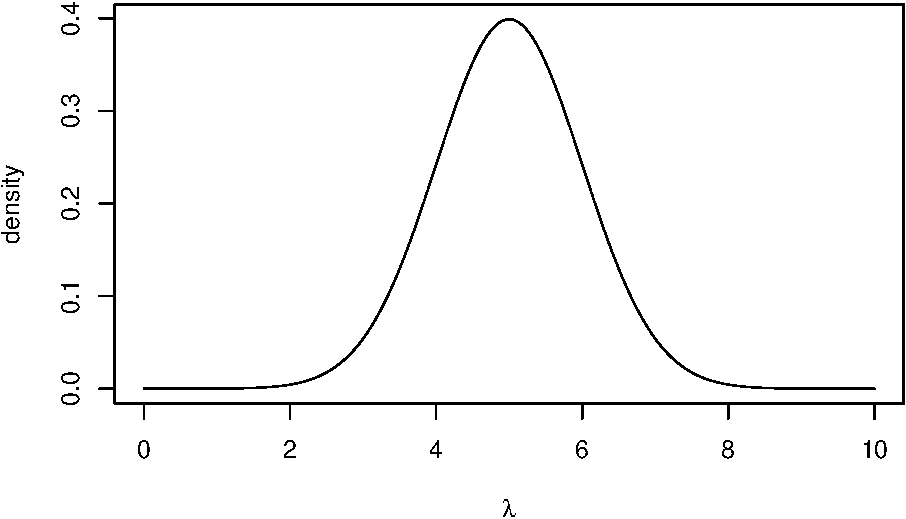
\includegraphics{_main_files/figure-latex/unnamed-chunk-18-1.pdf}
\end{example}

\hypertarget{rejection-sampling}{%
\section{Rejection Sampling}\label{rejection-sampling}}

We now have a way of sampling realisations from distributions where we can analytically derive the inverse distribution function. We can use this to sample from more complex densities, or simple densities more efficiently. Rejection sampling works by sampling according to a density we can sample from and then rejecting or accepting that sample based on the density we're actually interested in. The plot below shows an example from this. We would like to generate a sample from the distribution with the curved density function, which is challenging. Instead, we find a distribution whose density function bounds the one we are interested in a sample from that. In this case we can use the uniform distribution. Once we have generated our sample from he uniform distribution, we choose to accept or reject it based on the distribution we are interested in. In this case we reject it.

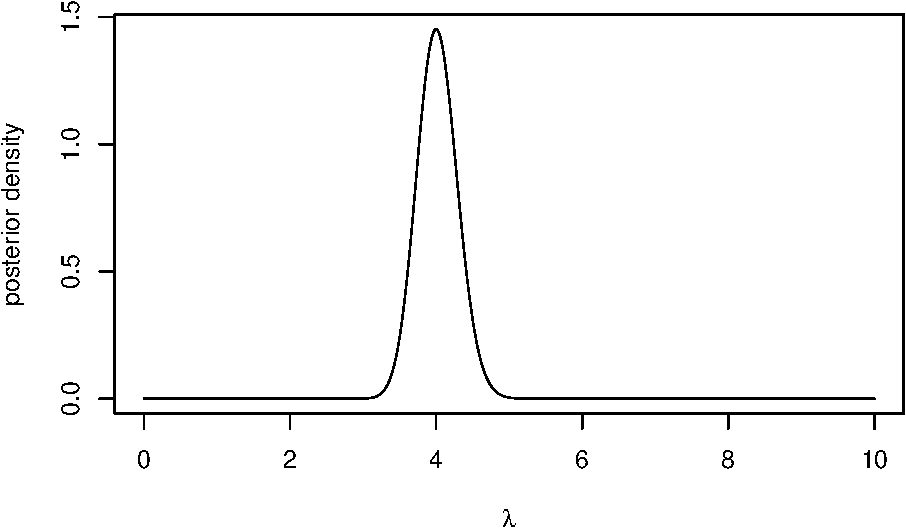
\includegraphics{_main_files/figure-latex/unnamed-chunk-19-1.pdf}

Suppose we want to sample from a density \(\pi\), but can only generate samples from a density \(q\). If there exists some constant \(c > 0\), such that \(\frac{\pi(y)}{q(y)} \leq c\) for all \(y\), then we can generate samples from \(p\) by

\begin{enumerate}
\def\labelenumi{\arabic{enumi}.}
\item
  Sampling \(Y \sim Q\)
\item
  Sampling \(U \sim U[0, 1]\)
\item
  Computing \(k = \frac{\pi(u)}{cq(y)}\)
\item
  Accepting \(y\) if \(U < k\) and rejecting otherwise.
\end{enumerate}

This says draw sample a point \(y\) according to the density \(q\). Draw a vertical line at \(y\) from the x-axis to \(cq(y)\). Sample uniformly on this line. If the uniformly random sample is below \(q\), then accept it. Otherwise, reject it. The theory behind this is as follows. Suppose we sample some point y according to this algorithm and we want to work out its density \(f\), then
\[
f(y) \propto q(y)\pi(U < k) = q(y)\frac{\pi(u)}{cq(y)} = \frac{\pi(u)}{c}.
\]
Therefore, \(f = p\).

\begin{example}
Suppose we want to sample from a distribution that has the density
\[
\pi(y) = \begin{cases}
\frac{3}{4}y(2-y), \qquad y \in [0, 2] \\
0, \qquad \textrm{otherwise}
\end{cases}.
\]
This has a maximum at \(\frac{3}{4}\). We choose \(p \sim U[0, 1]\) and \(c = \frac{3}{4}\). The R code below shows a pictorial version of how one sample is generated.

\begin{Shaded}
\begin{Highlighting}[]
\FunctionTok{set.seed}\NormalTok{(}\DecValTok{1234}\NormalTok{)   }\CommentTok{\#to reproduce}
\NormalTok{M }\OtherTok{\textless{}{-}} \DecValTok{3}\SpecialCharTok{/}\DecValTok{4}         \CommentTok{\#set M}
\NormalTok{y }\OtherTok{\textless{}{-}} \FunctionTok{runif}\NormalTok{(}\DecValTok{1}\NormalTok{)    }\CommentTok{\#sample Y \textasciitilde{} Q}
\NormalTok{p }\OtherTok{\textless{}{-}} \DecValTok{3}\SpecialCharTok{/}\DecValTok{4}\SpecialCharTok{*}\NormalTok{y}\SpecialCharTok{*}\NormalTok{(}\DecValTok{2}\SpecialCharTok{{-}}\NormalTok{y) }\CommentTok{\#compute pi(y)}
\NormalTok{k }\OtherTok{\textless{}{-}}\NormalTok{ p}\SpecialCharTok{/}\NormalTok{(M}\SpecialCharTok{*}\DecValTok{1}\NormalTok{)     }\CommentTok{\#compute k}
\NormalTok{u }\OtherTok{\textless{}{-}} \FunctionTok{runif}\NormalTok{(}\DecValTok{1}\NormalTok{)    }\CommentTok{\#sample U \textasciitilde{} U[0, 1]}
\FunctionTok{ifelse}\NormalTok{(u }\SpecialCharTok{\textless{}}\NormalTok{ k, }\StringTok{\textquotesingle{}accept\textquotesingle{}}\NormalTok{, }\StringTok{\textquotesingle{}reject\textquotesingle{}}\NormalTok{) }\CommentTok{\#Accept if  u \textless{} k}
\end{Highlighting}
\end{Shaded}

\begin{verbatim}
## [1] "reject"
\end{verbatim}

\begin{Shaded}
\begin{Highlighting}[]
\CommentTok{\#Create nice plot}
\NormalTok{a }\OtherTok{\textless{}{-}} \FunctionTok{seq}\NormalTok{(}\DecValTok{0}\NormalTok{, }\DecValTok{2}\NormalTok{, }\FloatTok{0.01}\NormalTok{)}
\NormalTok{b }\OtherTok{\textless{}{-}} \DecValTok{3}\SpecialCharTok{/}\DecValTok{4}\SpecialCharTok{*}\NormalTok{a}\SpecialCharTok{*}\NormalTok{(}\DecValTok{2}\SpecialCharTok{{-}}\NormalTok{a)}
\NormalTok{c }\OtherTok{\textless{}{-}}\NormalTok{ M}\SpecialCharTok{*}\FunctionTok{rep}\NormalTok{(}\DecValTok{1}\NormalTok{, }\FunctionTok{length}\NormalTok{(a))}
\FunctionTok{plot}\NormalTok{(a, b, }\AttributeTok{ylim =} \FunctionTok{c}\NormalTok{(}\DecValTok{0}\NormalTok{, M), }\AttributeTok{type =} \StringTok{\textquotesingle{}l\textquotesingle{}}\NormalTok{)}
\FunctionTok{lines}\NormalTok{(a, c)}
\FunctionTok{segments}\NormalTok{(}\AttributeTok{x0 =}\NormalTok{ y, }\AttributeTok{y0 =} \DecValTok{0}\NormalTok{, }\AttributeTok{x1 =}\NormalTok{ y,  }\AttributeTok{y1 =}\DecValTok{3}\SpecialCharTok{/}\DecValTok{4}\SpecialCharTok{*}\NormalTok{y}\SpecialCharTok{*}\NormalTok{(}\DecValTok{2}\SpecialCharTok{{-}}\NormalTok{y) , }\AttributeTok{lty =} \DecValTok{2}\NormalTok{, }\AttributeTok{lwd =} \DecValTok{2}\NormalTok{)}
\FunctionTok{segments}\NormalTok{(}\AttributeTok{x0 =}\NormalTok{ y,  }\AttributeTok{y0 =}\DecValTok{3}\SpecialCharTok{/}\DecValTok{4}\SpecialCharTok{*}\NormalTok{y}\SpecialCharTok{*}\NormalTok{(}\DecValTok{2}\SpecialCharTok{{-}}\NormalTok{y), }\AttributeTok{x1 =}\NormalTok{ y, }\AttributeTok{y1 =}\NormalTok{ M, }\AttributeTok{lty =} \DecValTok{2}\NormalTok{, }\AttributeTok{col =} \DecValTok{2}\NormalTok{, }\AttributeTok{lwd =} \DecValTok{2}\NormalTok{)}
\FunctionTok{points}\NormalTok{(}\AttributeTok{x =}\NormalTok{ y, }\AttributeTok{y =}\NormalTok{ u, }\AttributeTok{pch =} \DecValTok{19}\NormalTok{)}
\end{Highlighting}
\end{Shaded}

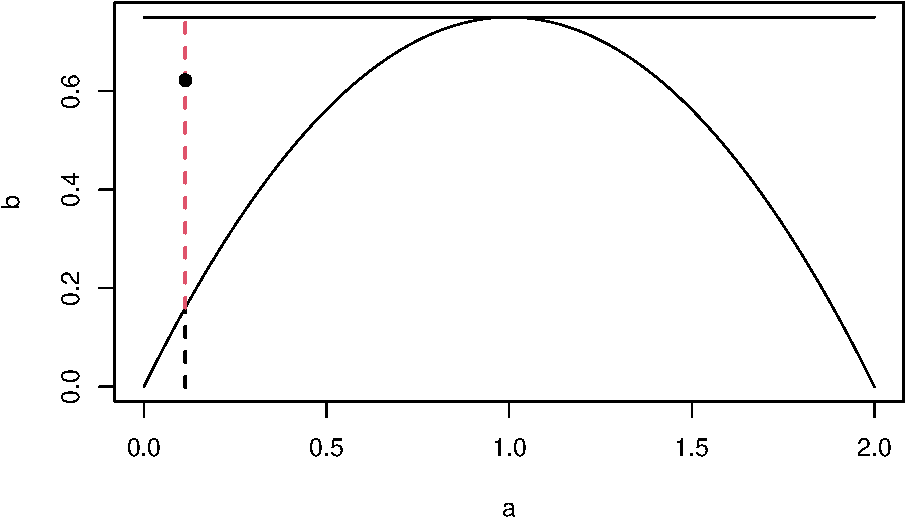
\includegraphics{_main_files/figure-latex/unnamed-chunk-20-1.pdf}
The plot also shows how the choices of \(M\) and \(q\) can make the sampling more or less efficient. In our example, the rejection space is large, meaning many of our proposed samples will be rejected. Here, we could have chosen a better \(q\) to minimise this space.
\end{example}

\hypertarget{markov-chain-monte-carlo}{%
\section{Markov Chain Monte Carlo}\label{markov-chain-monte-carlo}}

Markov Chain Monte Carlo (MCMC) is a class of algorithms that produce samples from a probability distribution. These methods combine the idea of rejection sampling with the theory of Markov chains. Before we set out the theory of Markov chains, we'll go through an example to show how MCMC works.

\begin{example}
\protect\hypertarget{exm:King}{}\label{exm:King}(\href{https://xcelab.net/rm/statistical-rethinking/}{Adapted from Statistical Rethinking \S 9}) Consider an eccentric King whose kingdom consists of a ring of 10 islands. Directly north is island one, the smallest island. Going clockwise around the archipelago, next is island two, which is twice the size of island one, then island three, which is three times as large as island one. Finally, island 10 is next to island one and ten times as large.

The King wanted to visit all of his islands, but spending time on each one according to its size. That is he should spend the most time on island ten and the least on island one. Being climate conscious, he also decided that flying from one side of the archipelago to the other was not allowed. Instead, he would only sail from one island to either of its neighbors. So from island one, he could reach islands two and ten.

He decided to travel according to these rules:

\begin{enumerate}
\def\labelenumi{\arabic{enumi}.}
\item
  At the end of each week, he decides to stay on the same island or move to a neighboring island according to a coin toss. If it's heads he proposes moving clockwise, and tails anti-clockwise. The island he is considering moving to is called the proposal island.
\item
  To decided if he is going to move to the proposal island, the King counts out a number of shells equal to the number of size of the island. So if island five is the proposal island, he counts out five shells. He then counts out a number of stones equal to the size of the current island.
\item
  If the number of seashells is greater than the number of stones, he moves to the proposed island. If the number of seashells is less than the number of stones, he takes a different strategy. He discards the number of stones equal to the number of seashells. So if there are six stone and five seashells, he ends up with 6-5=1 stones. He then places the stones and seashells into a bag a chooses one at random. If he picks a seashell, he moves to the proposed island, otherwise if he picks a shell, he stays put.
\end{enumerate}

This is a complex way of moving around, but it produces the required result; the time he spends on each island is proportionate to the size of the island. The code below shows an example of this over 10,000 weeks.

\begin{Shaded}
\begin{Highlighting}[]
\NormalTok{weeks }\OtherTok{\textless{}{-}} \DecValTok{10000}
\NormalTok{island }\OtherTok{\textless{}{-}} \FunctionTok{numeric}\NormalTok{(weeks)}
\NormalTok{current }\OtherTok{\textless{}{-}} \DecValTok{10}
\ControlFlowTok{for}\NormalTok{(i }\ControlFlowTok{in} \DecValTok{1}\SpecialCharTok{:}\NormalTok{weeks)\{}
  \DocumentationTok{\#\# record current position}
\NormalTok{  island[i] }\OtherTok{\textless{}{-}}\NormalTok{ current}
  
  \CommentTok{\#Flip a coin to move to a propose a new island}
\NormalTok{  proposed }\OtherTok{\textless{}{-}}\NormalTok{ current }\SpecialCharTok{+} \FunctionTok{sample}\NormalTok{(}\FunctionTok{c}\NormalTok{(}\DecValTok{1}\NormalTok{, }\SpecialCharTok{{-}}\DecValTok{1}\NormalTok{), }\AttributeTok{size =} \DecValTok{1}\NormalTok{)}
  
  \CommentTok{\#Ensure he loops round the island}
  \ControlFlowTok{if}\NormalTok{(proposed }\SpecialCharTok{\textless{}} \DecValTok{1}\NormalTok{) }
\NormalTok{    proposed }\OtherTok{\textless{}{-}} \DecValTok{10}
  \ControlFlowTok{if}\NormalTok{(proposed }\SpecialCharTok{\textgreater{}} \DecValTok{10}\NormalTok{)}
\NormalTok{    proposed }\OtherTok{\textless{}{-}} \DecValTok{1}
  
  \CommentTok{\#Decide to move}
\NormalTok{  p }\OtherTok{\textless{}{-}}\NormalTok{ proposed}\SpecialCharTok{/}\NormalTok{current}
\NormalTok{  u }\OtherTok{\textless{}{-}} \FunctionTok{runif}\NormalTok{(}\DecValTok{1}\NormalTok{)}
  \ControlFlowTok{if}\NormalTok{(u }\SpecialCharTok{\textless{}}\NormalTok{ p)}
\NormalTok{    current }\OtherTok{\textless{}{-}}\NormalTok{ proposed}
\NormalTok{\}}

\CommentTok{\#Plot results}
\FunctionTok{par}\NormalTok{(}\AttributeTok{mfrow =} \FunctionTok{c}\NormalTok{(}\DecValTok{2}\NormalTok{, }\DecValTok{1}\NormalTok{))}
\FunctionTok{plot}\NormalTok{(island, }\AttributeTok{type =} \StringTok{\textquotesingle{}l\textquotesingle{}}\NormalTok{, }\AttributeTok{xlab =} \StringTok{"Week"}\NormalTok{, }\AttributeTok{ylab =} \StringTok{"Island"}\NormalTok{)}
\FunctionTok{barplot}\NormalTok{(}\FunctionTok{table}\NormalTok{(island)}\SpecialCharTok{/}\NormalTok{weeks, }\AttributeTok{xlab =} \StringTok{"Island"}\NormalTok{, }\AttributeTok{ylab =} \StringTok{"Proportion of time"}\NormalTok{)}
\end{Highlighting}
\end{Shaded}

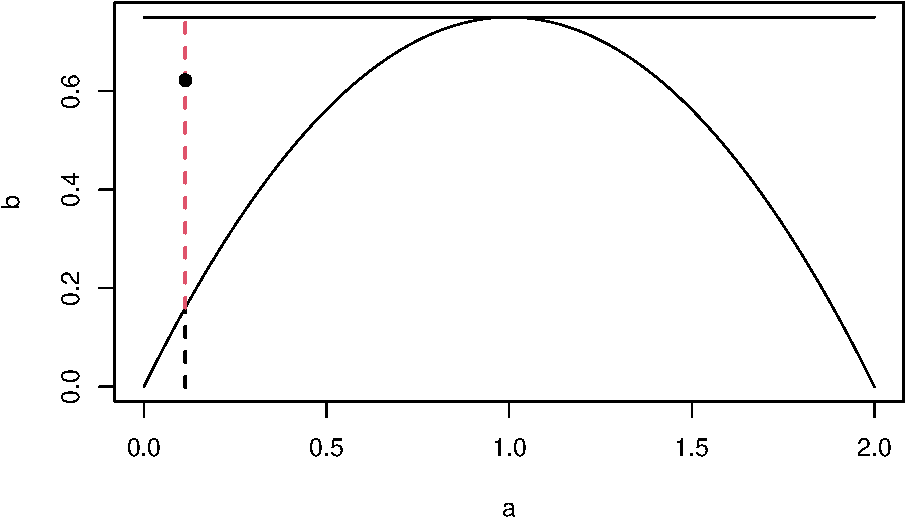
\includegraphics{_main_files/figure-latex/unnamed-chunk-21-1.pdf}
\end{example}

We can recognise several different statistical principles in this example. The King decides to move islands dependent on where he is currently, not based on where he has been previously (Markov property). He proposes an island to move to and accepts or rejects this decision based on some distribution (rejection principle). We are now going to describe some of the properties of Markov chains, including the Markov property.

\hypertarget{properties-of-markov-chains}{%
\section{Properties of Markov Chains}\label{properties-of-markov-chains}}

\begin{definition}
\protect\hypertarget{def:Markov}{}\label{def:Markov}A sequence of random variables \(\{Y_1, Y_2, \ldots\}\) is a \textbf{Markov chain} if \(\mathbb{P}(Y_{n+1} \mid Y_{n}, \ldots, Y_1) = \mathbb{P}(Y_{n+1} \mid Y_{n})\). That is that distribution of the next state \(Y_{n+1}\) only depends on the current state \(Y_n\) and not any previous states.
\end{definition}

\begin{definition}
The probability of transitioning from state \(i\) to state \(j\) in a Markov chain is given by \(p_{ij}\). The \textbf{transition matrix} for a Markov chain with \(N\) states is the \(N \times N\) matrix \(P\), where the \(\{i, j\}^{th}\) entry denoted by \(p_{ij}\) is probability is moving from state \(i\) to state \(j\).
\end{definition}

These two properties make Markov chains nice to work with, especially the Markov property (Definition \ref{def:Markov}). Two other important definitions are

\begin{definition}
The \textbf{period }of a state \(i\) is given by \(d_i = \textrm{gcd}\{n > 0; p_{ii} > 0 \}\). A state is \textbf{aperiodic} if \(d_i = 1\). An \textbf{aperiodic chain} is a chain where all states are a periodic.
\end{definition}

\begin{definition}
A Markov chain is \textbf{irreducible} if there exists an \(n \in \mathbb{N}\) such that \(\mathbb{P} (Y_n = i \mid Y_0 = j)\) for all pairs \(i\) and \(j\). In other words, it is possible to move from any state to any other state in a finite number of steps.
\end{definition}

We can use these definitions to start working with distributions. Suppose, the state we start at is drawn from some distribution \(Y_1 \sim \boldsymbol{q}\). Then the distributions of the second state \(Y_2\) depends on the distribution of \(Y_1\) and the transition probabilities
\[
\mathbb{P}(Y_2 = j) = \sum_i q_ip_{ij}.
\]
If we denote the distribution of \(Y_2 \sim \boldsymbol{q}^{(2)}\), then we can write it in terms of the transition matrix \(\boldsymbol{q}^\prime = \boldsymbol{q}P\). Now suppose we would like the distribution of \(Y_3 \sim \boldsymbol{q}^{(3)}\), thanks to the Markov property, this is the distribution for \(Y_2\) multiplied by the transition matrix, so \(Y_3 \sim qP^2\). Inductively, \(P_k \sim qP^{k-1}\). To use Markov chains to sample from distributions, we need to identify the Eigenvalues of the transition matrix.

\begin{proposition}
A transition matrix \(P\) always has at least one eigenvalue equal to one.
\end{proposition}

\begin{proof}
The columns of \(P\) sum to 1 as they are probability distributions. Therefore, \(1\) is an eigenvalue.
\end{proof}

\begin{definition}
If a transition matrix \(P\) has a unique Eigenvalue that takes the value 1, there is a unique distribution \(\pi\) such that
\[
\pi P = \pi. 
\]
This distribution \(\pi\), is known as the \textbf{stationary distribution}.
\end{definition}

This important concept underpins MCMC methods. It says that no matter where we start our chain, we'll eventually end up sampling states according to the distribution \(\pi\). It make take a long time to reach the stationary distribution, but it will eventually get there.

In order to check whether our Markov chain will converge to a stationary distribution, we need to check:

\begin{enumerate}
\def\labelenumi{\arabic{enumi}.}
\item
  the Markov chain is aperiodic,
\item
  the Markov chain is irreducible, and
\item
  that there exists a unique distribution \(\pi\) such that \(\pi P = \pi\).
\end{enumerate}

\begin{example}
In Example \ref{exm:King}, the King wanted to visit the islands according to how large they are. We can think of the islands as the states and the stationary distribution as \(p(Y = i) \propto i\). The eccentric method the King used allowed him to construct a transition matrix for an aperiodic Markov chain. He also never visited islands regularly using this method.
\end{example}

When designing a Markov chain, it is usually straightforward to design one that meets conditions one and two. Condition three is more difficult to prove, but for some chains it is possible to show they satisfy detailed balance.

\begin{definition}
The Markov chain with transition matrix \(P\) satisfies the \textbf{detailed balance} equation with respect to the distribution \(\pi\) if
\[
\pi_i p_{ij} = \pi_j p_{ji}. 
\]
\end{definition}

\begin{theorem}[Detailed Balance]
Let \(P\) be a transition matrix that satisfies detailed balance with respect to the distribution \(\pi\). Then \(\pi P = \pi\).
\end{theorem}

\begin{proof}
The \(j^{th}\) row of \(\pi P\) is
\begin{align*}
\sum_{i} \pi_i p_{ij} & = \sum_{i} \pi_j p_{ji} \quad \textrm{(detailed balance)} \\
 & = \pi_j \sum_{i} p_{ji} \\
 & = \pi_j.\qquad \textrm{(probaility sums to 1)}
\end{align*}
Hence \(\pi P = \pi\).
\end{proof}

The section has shown us that we can use a Markov chain theory to simulate from a probability distribution \(\pi\). All we need is for the Markov chain to be irreducible, aperiodic, and for the transition matrix to satisfy \(\pi P = \pi\). This provides the foundation theory for MCMC and allows us to sample from a posterior distribution \(\pi\). What it doesn't tell us is how to design the Markov chain, and that is what the next sections deal with.

\hypertarget{metropolis-hastings}{%
\section{Metropolis-Hastings}\label{metropolis-hastings}}

We're now going to look at MCMC algorithms. The first algorithm we are going to look at is the Metropolis-Hasting algorithm. This is a useful algorithm if we cannot sample directly from the posterior distribution and if the conditional distributions do not have a closed form. The Metropolis-Hastings algorithm is like the island example we saw earlier. At each iteration, we propose a new sample and then accept or reject it based on the likelihood function, the prior and how likely we are to propose this new sample given the current one.

Suppose we want to sample from the posterior distribution \(\pi(\theta \mid \boldsymbol{y})\). The Metropolis-Hastings works as follows:

\begin{enumerate}
\def\labelenumi{\arabic{enumi}.}
\item
  Set the initial value \(\theta^{(0)}\).
\item
  Set \(i = 1\).
\item
  Propose a new value of \(\theta'\) from some distribution \(q\)
\item
  Accept \(\theta'\) with probability
  \[
  p_{\textrm{acc}} = \min\left\{\frac{\pi(\theta' \mid \boldsymbol{y})}{\pi(\theta \mid \boldsymbol{y})}\frac{q(\theta \mid \theta')}{q(\theta' \mid \theta)}, 1\right\}.
  \]
\item
  Repeat steps 3 to 4 for \(i = 2, \ldots, M\).
\end{enumerate}

There are two parts to the acceptance probability in step 4. The first is the posterior ratio, similar to saying the likelihood of \(\theta'\) given the observed data over the likelihood of \(\theta\) given the data. The second is the proposal ratio. It is similar to saying the likelihood of proposing \(\theta\) given the current value \(\theta'\), over the likelihood of proposing \(\theta'\) given the current value \(\theta\).

In practice, we don't need to evaluate the full posterior distribution. Recall
\[
\pi(\theta \mid \boldsymbol{y}) = \frac{\pi(\boldsymbol{y} \mid \theta) \pi(\theta)}{\pi(y)}
\]
As the the denominator doesn't depend on \(\theta\), it cancels in the ration. The ratio becomes
\[
\frac{\pi(\theta' \mid \boldsymbol{y})}{\pi(\theta \mid \boldsymbol{y})} = \frac{\pi(\boldsymbol{y} \mid \theta') \pi(\theta')}{\pi(\boldsymbol{y} \mid \theta) \pi(\theta)}.
\]
This is the likelihood ratio multiplied by the prior ratio.

\begin{proposition}
The Markov chain generated by the Metropolis-Hastings algorithm satisfies detailed balance with respect to the posterior distribution.
\end{proposition}

\begin{proof}
Denote the current state \(\theta\) and the proposed state \(\theta'\). We would like to show
\[
\pi(\theta \mid \boldsymbol{y}) \pi(\theta'\mid\theta) = \pi(\theta' \mid \boldsymbol{y}) \pi(\theta\mid\theta').
\]
The density of \(\theta'\) given the proposed state \(\theta\) is the proposal density multiplied by the acceptance probability. It is given by
\begin{align*}
\pi(\theta' \mid \theta) &= q(\theta' \mid \theta)p_{acc}\\
&=  q(\theta' \mid \theta)\min\left\{\frac{\pi(\theta' \mid \boldsymbol{y})}{\pi(\theta' \mid \boldsymbol{y})}\frac{q(\theta \mid \theta')}{q(\theta' \mid \theta)}, \, 1\right\} \\
& = \min\left\{\frac{\pi(\theta' \mid \boldsymbol{y})}{\pi(\theta' \mid \boldsymbol{y})}q(\theta \mid \theta'),\, q(\theta' \mid \theta)\right\}.
\end{align*}

The left hand side of the detailed balance equation becomes
\[
\pi(\theta \mid \boldsymbol{y})\pi(\theta' \mid \theta) = \min\{\pi(\theta' \mid \boldsymbol{y})q(\theta \mid \theta'),\, \pi(\theta \mid \boldsymbol{y})q(\theta' \mid \theta)\}.
\]
Analogously, we can show the right hand side is

\[
\pi(\theta' \mid \boldsymbol{y})\pi(\theta \mid \theta') = \min\{\pi(\theta' \mid \boldsymbol{y})q(\theta \mid \theta'),\, \pi(\theta \mid \boldsymbol{y})q(\theta' \mid \theta)\}.
\]
Hence, \(\pi(\theta \mid \boldsymbol{y}) \pi(\theta'\mid\theta) = \pi(\theta' \mid \boldsymbol{y}) \pi(\theta\mid\theta')\) and the Markov chain satisfies detailed balance with respect to the posterior disquisition.
\end{proof}

\begin{example}
\protect\hypertarget{exm:norm}{}\label{exm:norm}Lets think again about the reaction time example in the previous chapter.The time until each lorry driver reacts (in milliseconds) is

\begin{Shaded}
\begin{Highlighting}[]
\NormalTok{y }\OtherTok{\textless{}{-}} \FunctionTok{c}\NormalTok{(}\FloatTok{0.34}\NormalTok{, }\FloatTok{0.47}\NormalTok{, }\FloatTok{0.58}\NormalTok{, }\FloatTok{0.27}\NormalTok{, }\FloatTok{0.74}\NormalTok{, }\FloatTok{0.44}\NormalTok{, }\FloatTok{0.46}\NormalTok{, }\FloatTok{0.65}\NormalTok{, }\FloatTok{0.36}\NormalTok{, }\FloatTok{0.55}\NormalTok{, }\FloatTok{0.58}\NormalTok{, }\FloatTok{0.55}\NormalTok{, }\FloatTok{0.53}\NormalTok{, }\FloatTok{0.56}\NormalTok{, }\FloatTok{0.54}\NormalTok{, }\FloatTok{0.61}\NormalTok{, }\FloatTok{0.43}\NormalTok{, }\FloatTok{0.52}\NormalTok{, }\FloatTok{0.45}\NormalTok{, }\FloatTok{0.49}\NormalTok{, }\FloatTok{0.32}\NormalTok{, }\FloatTok{0.33}\NormalTok{, }\FloatTok{0.47}\NormalTok{, }\FloatTok{0.58}\NormalTok{, }\FloatTok{0.34}\NormalTok{, }\FloatTok{0.60}\NormalTok{, }\FloatTok{0.59}\NormalTok{, }\FloatTok{0.43}\NormalTok{, }\FloatTok{0.57}\NormalTok{, }\FloatTok{0.34}\NormalTok{)}
\FunctionTok{hist}\NormalTok{(y, }\AttributeTok{main =} \StringTok{""}\NormalTok{, }\AttributeTok{xlab =} \StringTok{"Reaction time (ms)"}\NormalTok{)}
\end{Highlighting}
\end{Shaded}

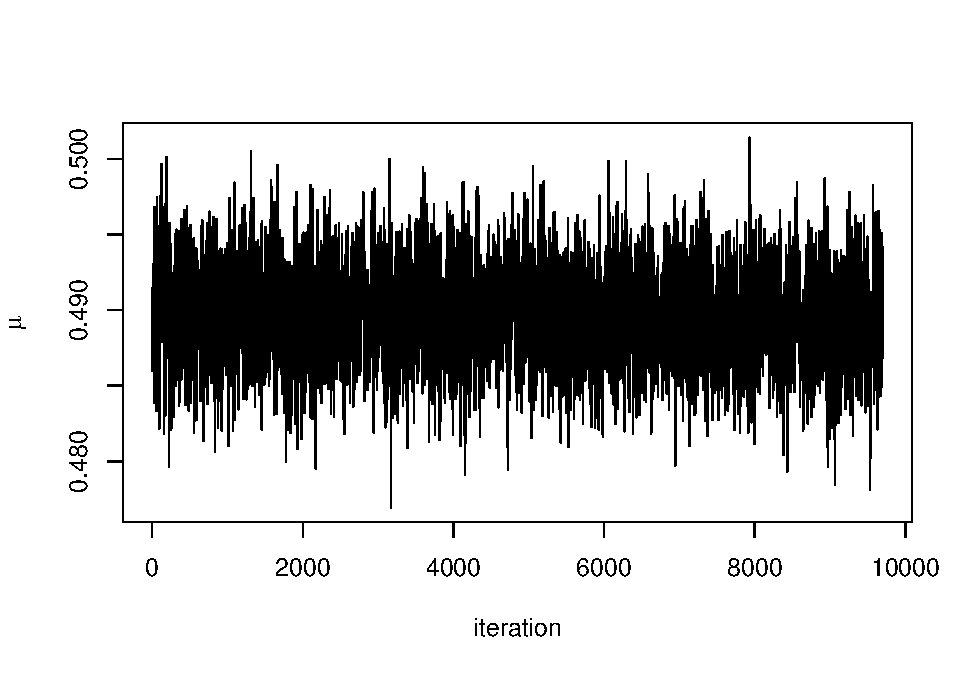
\includegraphics{_main_files/figure-latex/unnamed-chunk-22-1.pdf}

Assuming \(Y_i \sim N(\mu, \sigma^2)\) are independent and identically distributed for \(i=1,...,n\), by Bayes' theorem, the posterior distribution is

\[
\pi(\mu \mid \boldsymbol{y}, \sigma^2) \propto \pi(\boldsymbol{y} \mid \mu, \sigma^2) \pi(\mu).
\]
One of the issues here is that we have assigned a normal prior distribution to the population mean parameter \(\mu\). The advantage previously was that we could derive a posterior distribution with closed form. The disadvantage however is that the choice of prior distribution assigns some positive probability to impossible values of \(\mu\), i.e.~reaction times less than zero.

Now we have a tool to sample from posterior distributions that don't have a closed form. We can instead assign an exponential prior distribution, a distribution which only has non-negative support. Letting \(\mu \sim \textrm{Exp}(0.01)\) sets a vague prior distribution on \(\mu\). It can be shown that the posterior distribution (exercise) is therefore
\[
\pi(\mu \mid \boldsymbol{y}, \sigma^2) \propto \exp\left\{-0.01\mu -\sum_{i=1}^{30}\frac{(y_i - \mu)^2}{\sigma^2}\right\} 
\]

We can use the Metropolis-Hasting algorithm to sample from this posterior distribution. But how should we propose new value of \(\mu\)? A common method is a Metropolis-Hastings Random Walk proposal distribution. The proposal distribution is symmetric and centered on \(\mu\). The two most common methods are \(\mu' \mid \mu \sim U[\mu - \varepsilon, \mu + \varepsilon]\) and \(\mu' \mid \mu \sim N(\mu, \tau^2)\). We choose the uniform proposal distribution, with
\[
q(\mu' \mid \mu) = \frac{1}{2\varepsilon}.
\]

The acceptance probability is therefore
\[
p_\textrm{acc} = \min\left\{\frac{\exp\left\{-0.01\mu' -\sum_{i=1}^{30}\frac{(y_i - \mu')^2}{\sigma^2}\right\} }{\exp\left\{-0.01\mu -\sum_{i=1}^{30}\frac{(y_i - \mu)^2}{\sigma^2}\right\} }, 1\right\}
\]

We can implement a sampler in R as follows:

\begin{Shaded}
\begin{Highlighting}[]
\CommentTok{\#Set up elements for MCMC}
\FunctionTok{set.seed}\NormalTok{(}\DecValTok{123}\NormalTok{) }\CommentTok{\#to reproduce}
\NormalTok{n.iter   }\OtherTok{\textless{}{-}} \DecValTok{10000}
\NormalTok{mu.store }\OtherTok{\textless{}{-}} \FunctionTok{numeric}\NormalTok{(n.iter)}

\CommentTok{\#Initial values}
\NormalTok{mu }\OtherTok{\textless{}{-}} \DecValTok{1} 
\NormalTok{sigma }\OtherTok{\textless{}{-}} \FloatTok{0.1} \CommentTok{\#known}

\ControlFlowTok{for}\NormalTok{(i }\ControlFlowTok{in} \DecValTok{1}\SpecialCharTok{:}\NormalTok{n.iter)\{}
  
  \CommentTok{\#Propose value for mu}
\NormalTok{  mu.proposed }\OtherTok{\textless{}{-}} \FunctionTok{runif}\NormalTok{(}\DecValTok{1}\NormalTok{, mu }\SpecialCharTok{{-}} \FloatTok{0.01}\NormalTok{, mu }\SpecialCharTok{+} \FloatTok{0.01}\NormalTok{)}
  
  \ControlFlowTok{if}\NormalTok{(mu.proposed }\SpecialCharTok{\textgreater{}} \DecValTok{0}\NormalTok{)\{ }\CommentTok{\#If mu \textless{} 0 we can reject straight away}
    
    \CommentTok{\#Compute (log) acceptance probability}
\NormalTok{    log.numerator   }\OtherTok{\textless{}{-}} \SpecialCharTok{{-}}\FloatTok{0.01}\SpecialCharTok{*}\NormalTok{mu.proposed }\SpecialCharTok{{-}} \FunctionTok{sum}\NormalTok{(y }\SpecialCharTok{{-}}\NormalTok{ mu.proposed)}\SpecialCharTok{\^{}}\DecValTok{2}\SpecialCharTok{/}\NormalTok{(}\DecValTok{2}\SpecialCharTok{*}\NormalTok{sigma}\SpecialCharTok{\^{}}\DecValTok{2}\NormalTok{)}
\NormalTok{    log.denominator }\OtherTok{\textless{}{-}} \SpecialCharTok{{-}}\FloatTok{0.01}\SpecialCharTok{*}\NormalTok{mu }\SpecialCharTok{{-}} \FunctionTok{sum}\NormalTok{(y }\SpecialCharTok{{-}}\NormalTok{ mu)}\SpecialCharTok{\^{}}\DecValTok{2}\SpecialCharTok{/}\NormalTok{(}\DecValTok{2}\SpecialCharTok{*}\NormalTok{sigma}\SpecialCharTok{\^{}}\DecValTok{2}\NormalTok{)}
    
\NormalTok{    log.p.acc }\OtherTok{\textless{}{-}}\NormalTok{ log.numerator }\SpecialCharTok{{-}}\NormalTok{ log.denominator}
\NormalTok{    u }\OtherTok{\textless{}{-}} \FunctionTok{runif}\NormalTok{(}\DecValTok{1}\NormalTok{)}
    
    \CommentTok{\#Accept/Reject step}
    \ControlFlowTok{if}\NormalTok{(}\FunctionTok{log}\NormalTok{(u) }\SpecialCharTok{\textless{}}\NormalTok{ log.p.acc)\{}
\NormalTok{      mu }\OtherTok{\textless{}{-}}\NormalTok{ mu.proposed}
\NormalTok{    \}}
\NormalTok{  \}}
  
  \CommentTok{\#Store mu at each iteration}
\NormalTok{  mu.store[i] }\OtherTok{\textless{}{-}}\NormalTok{ mu}
\NormalTok{\}}
\FunctionTok{plot}\NormalTok{(mu.store, }\AttributeTok{type =} \StringTok{\textquotesingle{}l\textquotesingle{}}\NormalTok{, }\AttributeTok{xlab =} \StringTok{"iteration"}\NormalTok{, }\AttributeTok{ylab =} \FunctionTok{expression}\NormalTok{(mu))}
\end{Highlighting}
\end{Shaded}

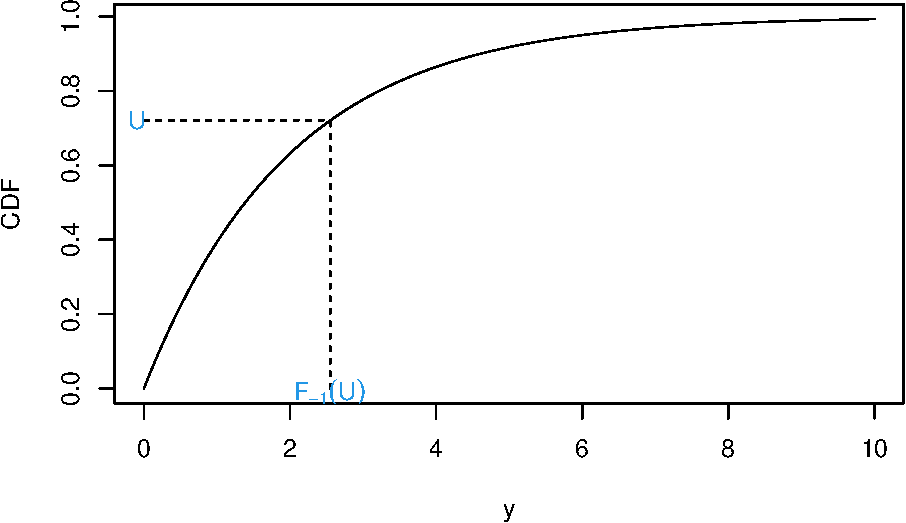
\includegraphics{_main_files/figure-latex/unnamed-chunk-23-1.pdf}

We can see that after about 300 iterations, the Markov chain has converged to its stationary distribution, the posterior distribution. We can see this more clearly by removing the first 300 iterations.

\begin{Shaded}
\begin{Highlighting}[]
\FunctionTok{plot}\NormalTok{(mu.store[}\SpecialCharTok{{-}}\FunctionTok{c}\NormalTok{(}\DecValTok{1}\SpecialCharTok{:}\DecValTok{300}\NormalTok{)], }\AttributeTok{type =} \StringTok{\textquotesingle{}l\textquotesingle{}}\NormalTok{, }\AttributeTok{xlab =} \StringTok{"iteration"}\NormalTok{, }\AttributeTok{ylab =} \FunctionTok{expression}\NormalTok{(mu))}
\end{Highlighting}
\end{Shaded}

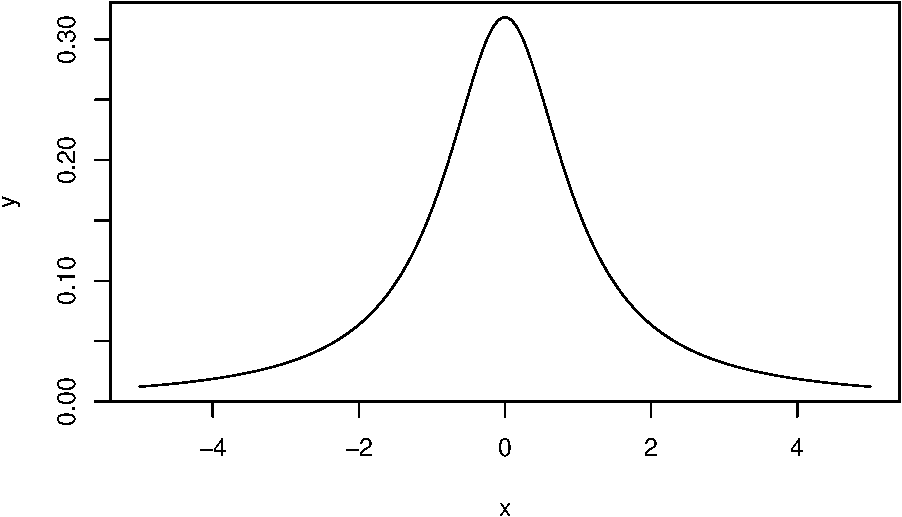
\includegraphics{_main_files/figure-latex/unnamed-chunk-24-1.pdf}

\begin{Shaded}
\begin{Highlighting}[]
\FunctionTok{hist}\NormalTok{(mu.store[}\SpecialCharTok{{-}}\FunctionTok{c}\NormalTok{(}\DecValTok{1}\SpecialCharTok{:}\DecValTok{300}\NormalTok{)], }\AttributeTok{xlab =} \FunctionTok{expression}\NormalTok{(mu), }\AttributeTok{main =} \StringTok{"Posterior distribution"}\NormalTok{)}
\end{Highlighting}
\end{Shaded}

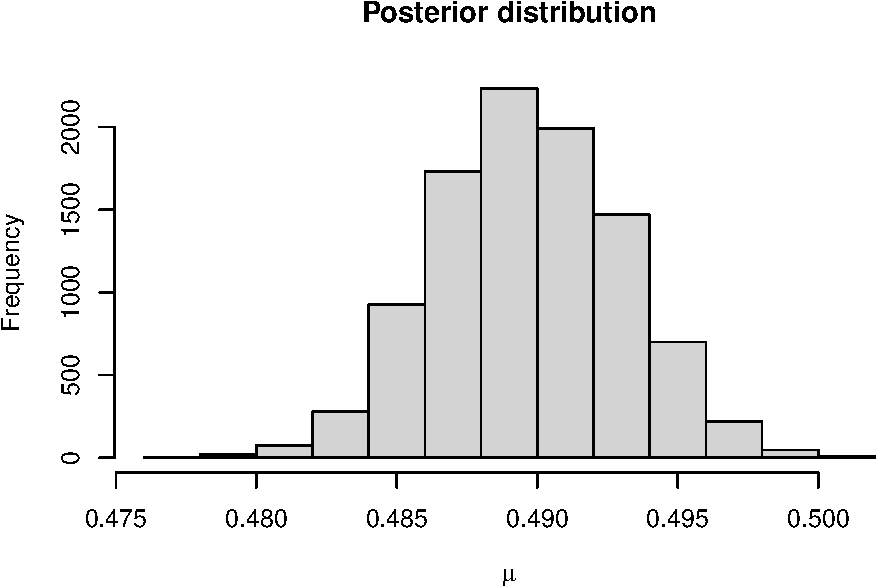
\includegraphics{_main_files/figure-latex/unnamed-chunk-24-2.pdf}

The 95\% credible interval for \(\mu\) using this prior distribution is

\begin{Shaded}
\begin{Highlighting}[]
\FunctionTok{quantile}\NormalTok{(mu.store[}\SpecialCharTok{{-}}\FunctionTok{c}\NormalTok{(}\DecValTok{1}\SpecialCharTok{:}\DecValTok{300}\NormalTok{)], }\FunctionTok{c}\NormalTok{(}\FloatTok{0.025}\NormalTok{, }\FloatTok{0.975}\NormalTok{))}
\end{Highlighting}
\end{Shaded}

\begin{verbatim}
##      2.5%     97.5% 
## 0.4832146 0.4961484
\end{verbatim}

Recall that using the normal prior distribution, it was

\begin{verbatim}
0.486 0.493
\end{verbatim}

It seems that the posterior distribution is very similar when using these two prior distributions. This is because the data are very informative.
\end{example}

\hypertarget{gibbs-sampler}{%
\section{Gibbs Sampler}\label{gibbs-sampler}}

When we can sample directly from conditional posterior distributions, we can use a Gibbs sampler. Suppose we have a distribution with parameters \(\{\theta_1, \ldots, \theta_N\}\), a Gibbs sampler works as follows:

\begin{enumerate}
\def\labelenumi{\arabic{enumi}.}
\item
  Set initial values \(\{\theta_1^{(0)}, \ldots, \theta_N^{(0)}\}\)
\item
  Set \(i = 1\).
\item
  Draw a value for \(\theta_1^{(i)}\) from \(\pi(\theta_1 \mid \theta_2^{(i-1)}, \ldots, \theta_N^{(i-1)}))\).
\item
  Draw a value for \(\theta_2^{(i)}\) from \(\pi(\theta_2 \mid \theta_1^{(i-1)}, \theta_3^{(i-1)}, \ldots, \theta_N^{(i-1)}))\).
\item
  Repeat steps 3 and 4 for parameters \(\{\theta_3^{(i)}, \ldots, \theta_N^{(i)}\}\).
\item
  Repeat steps 3, 4, and 5, for \(i = 2, \ldots M\).
\end{enumerate}

In code, this might look like

\begin{verbatim}
M #number of iterations
N #number of parameters
theta.store   <- matrix(NA, N, M)
theta         <- numeric(N)

for(j in 1:M){
  for(j in 1:N){
    theta[i] <- #sample from conditional with theta[-i]
  }
  theta.store[, j] <- theta.current #store current values
}
\end{verbatim}

The sequence \(\left\{\theta_0^{(0)},\ldots, \theta_N^{(0)}\right\}, \left\{\theta_0^{(1)},\ldots, \theta_N^{(1)}\right\}, \ldots, \left\{\theta_0^{(M)},\ldots, \theta_N^{(M)}\right\}\) form a Markov chain. They also form a series of samples from the posterior distribution. However it is important to note that by construction, these samples are not independent since each realisation depends on the previous sample and we must take this into account when doing estimation.

\begin{example}

Recall the lab in the previous chapter where we derived the posterior distribution for the mean \(\mu\) and variance \(\sigma^2\) for normally distributed data. The marginal posterior distributions are given by
\[
\mu \mid \boldsymbol{y}, \sigma^2 \sim N(\mu_1, \sigma^2_1),
\]

\[
\sigma^2 \mid \boldsymbol{y}, \mu \sim \textrm{inv-Gamma}\left(\alpha + \frac{N}{2}, \,\beta + \frac{\sum_{i=1}^N (y_i - \mu)^2}{2}\right),
\]

where \(\mu_1 =\left(\frac{\sum_{i=1}^{30}y_i}{\sigma^2} + \frac{\mu_0}{\sigma_0^2} \right)\) and \(\sigma^2_1 = \left(\frac{30}{\sigma^2} + \frac{1}{\sigma_0^2}\right)^{-1}\).

We can set up a Metropolis-Hastings algorithm using Gibbs samplers to generate samples for \(\lambda\) and \(\gamma\).

\begin{enumerate}
\def\labelenumi{\arabic{enumi}.}
\item
  Set initial values \(\{\lambda^{(0)}, \gamma^{(0)}\}\)
\item
  Set \(i = 1\).
\item
  Draw a value for \(\lambda^{(i)} \mid \boldsymbol{y}, \gamma^{(i-1)} \sim \textrm{Gamma}(10, 95 + \gamma^{(i-1)})\)
\item
  Draw a value for \(\gamma^{(i)} \mid \boldsymbol{y}, \,\lambda^{(i)} \sim \hbox{Exp}(\lambda^{(i)} + \nu)\).
\item
  Repeat steps 3 and 4 for \(i = 2, \ldots M\).
\end{enumerate}

\end{example}

\hypertarget{mcmc-diagnostics}{%
\section{MCMC Diagnostics}\label{mcmc-diagnostics}}

When running an MCMC algorithm, it is always important to check that the Markov chain has converged and is mixing well. For our purposes, mixing well means the chain is exploring the space of possible values of \(\theta\) effectively and effectively and not getting stuck on the same value for a long time.

A key way of doing this is by looking at the trace plot, which is a time series of the posterior samples simulated by the algorithm. The trace plot should look like it has converged to the stationary distribution and exploring the stationary distribution efficiently. What it shouldn't look like is a long series of small steps, or being stuck in one spot for a long time. There are two definitions that help us isolate an efficient Markov chain.

\begin{definition}
The \textbf{burn-in period} is the number of iterations the Markov chain takes to reach the stationary distribution.
\end{definition}

\begin{definition}
The \textbf{thinning parameter} is the period of iterations of the Markov chain that are stored.
\end{definition}

\begin{example}
In Example @\{exm:norm\}, we saw a Markov chain that mixes well. We took the burn-in period to be 3,000 iterations, which was how long it took to for the chain to converge.

In a Metropolis-Hasting random walk algorithm, the proposal distribution often has a large impact on how well the Markov chain mixes. The variance, or step size, of the proposal distribution can be tuned to ensure the chain mixes well.

The following two examples show poorly mixing Markov chains. The first is where the step size is too big and the chain frequently gets stuck for several hundred iterations.

\begin{Shaded}
\begin{Highlighting}[]
\FunctionTok{set.seed}\NormalTok{(}\DecValTok{123}\NormalTok{) }\CommentTok{\#to reproduce}
\NormalTok{n.iter   }\OtherTok{\textless{}{-}} \DecValTok{10000}
\NormalTok{mu.store }\OtherTok{\textless{}{-}} \FunctionTok{numeric}\NormalTok{(n.iter)}

\CommentTok{\#Initial values}
\NormalTok{mu }\OtherTok{\textless{}{-}} \DecValTok{1} 
\NormalTok{sigma }\OtherTok{\textless{}{-}} \FloatTok{0.1} \CommentTok{\#known}

\ControlFlowTok{for}\NormalTok{(i }\ControlFlowTok{in} \DecValTok{1}\SpecialCharTok{:}\NormalTok{n.iter)\{}
  
  \CommentTok{\#Propose value for mu}
\NormalTok{  mu.proposed }\OtherTok{\textless{}{-}} \FunctionTok{runif}\NormalTok{(}\DecValTok{1}\NormalTok{, mu }\SpecialCharTok{{-}} \FloatTok{0.1}\NormalTok{, mu }\SpecialCharTok{+} \FloatTok{0.1}\NormalTok{) }\CommentTok{\#Step size too big}
  
  \ControlFlowTok{if}\NormalTok{(mu.proposed }\SpecialCharTok{\textgreater{}} \DecValTok{0}\NormalTok{)\{ }\CommentTok{\#If mu \textless{} 0 we can reject straight away}
    
    \CommentTok{\#Compute (log) acceptance probability}
\NormalTok{    log.numerator   }\OtherTok{\textless{}{-}} \SpecialCharTok{{-}}\FloatTok{0.01}\SpecialCharTok{*}\NormalTok{mu.proposed }\SpecialCharTok{{-}} \FunctionTok{sum}\NormalTok{(y }\SpecialCharTok{{-}}\NormalTok{ mu.proposed)}\SpecialCharTok{\^{}}\DecValTok{2}\SpecialCharTok{/}\NormalTok{(}\DecValTok{2}\SpecialCharTok{*}\NormalTok{sigma}\SpecialCharTok{\^{}}\DecValTok{2}\NormalTok{)}
\NormalTok{    log.denominator }\OtherTok{\textless{}{-}} \SpecialCharTok{{-}}\FloatTok{0.01}\SpecialCharTok{*}\NormalTok{mu }\SpecialCharTok{{-}} \FunctionTok{sum}\NormalTok{(y }\SpecialCharTok{{-}}\NormalTok{ mu)}\SpecialCharTok{\^{}}\DecValTok{2}\SpecialCharTok{/}\NormalTok{(}\DecValTok{2}\SpecialCharTok{*}\NormalTok{sigma}\SpecialCharTok{\^{}}\DecValTok{2}\NormalTok{)}
    
\NormalTok{    log.p.acc }\OtherTok{\textless{}{-}}\NormalTok{ log.numerator }\SpecialCharTok{{-}}\NormalTok{ log.denominator}
\NormalTok{    u }\OtherTok{\textless{}{-}} \FunctionTok{runif}\NormalTok{(}\DecValTok{1}\NormalTok{)}
    
    \CommentTok{\#Accept/Reject step}
    \ControlFlowTok{if}\NormalTok{(}\FunctionTok{log}\NormalTok{(u) }\SpecialCharTok{\textless{}}\NormalTok{ log.p.acc)\{}
\NormalTok{      mu }\OtherTok{\textless{}{-}}\NormalTok{ mu.proposed}
\NormalTok{    \}}
\NormalTok{  \}}
  
  \CommentTok{\#Store mu at each iteration}
\NormalTok{  mu.store[i] }\OtherTok{\textless{}{-}}\NormalTok{ mu}
\NormalTok{\}}
\FunctionTok{plot}\NormalTok{(mu.store[}\SpecialCharTok{{-}}\FunctionTok{c}\NormalTok{(}\DecValTok{1}\SpecialCharTok{:}\DecValTok{3000}\NormalTok{)], }\AttributeTok{type =} \StringTok{\textquotesingle{}l\textquotesingle{}}\NormalTok{, }\AttributeTok{xlab =} \StringTok{"iteration"}\NormalTok{, }\AttributeTok{ylab =} \FunctionTok{expression}\NormalTok{(mu))}
\end{Highlighting}
\end{Shaded}

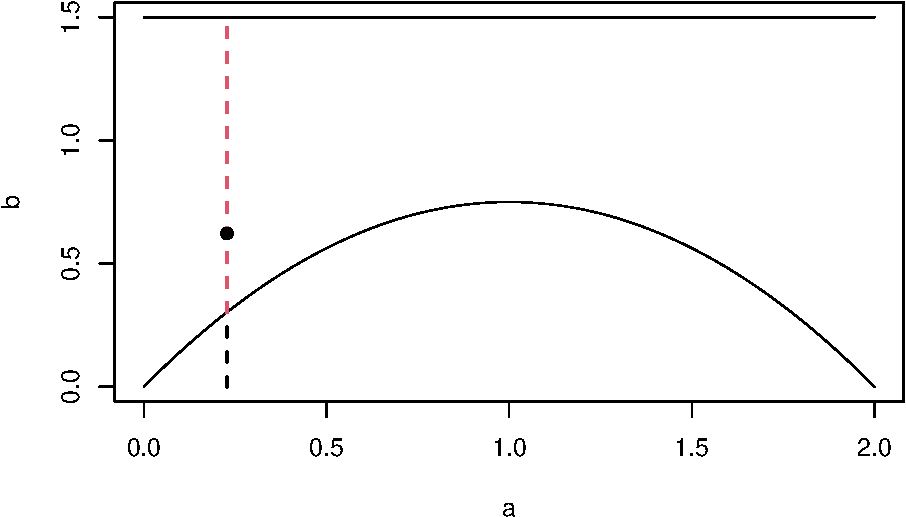
\includegraphics{_main_files/figure-latex/unnamed-chunk-26-1.pdf}

The next is where the step size is too small. It takes a long time for the chain to converge (\textasciitilde50\% of the run time). When the chain does converge, it is inefficient at exploring the space.

\begin{Shaded}
\begin{Highlighting}[]
\FunctionTok{set.seed}\NormalTok{(}\DecValTok{123}\NormalTok{) }\CommentTok{\#to reproduce}
\NormalTok{n.iter   }\OtherTok{\textless{}{-}} \DecValTok{10000}
\NormalTok{mu.store }\OtherTok{\textless{}{-}} \FunctionTok{numeric}\NormalTok{(n.iter)}

\CommentTok{\#Initial values}
\NormalTok{mu }\OtherTok{\textless{}{-}} \DecValTok{1} 
\NormalTok{sigma }\OtherTok{\textless{}{-}} \FloatTok{0.1} \CommentTok{\#known}

\ControlFlowTok{for}\NormalTok{(i }\ControlFlowTok{in} \DecValTok{1}\SpecialCharTok{:}\NormalTok{n.iter)\{}
  
  \CommentTok{\#Propose value for mu}
\NormalTok{  mu.proposed }\OtherTok{\textless{}{-}} \FunctionTok{runif}\NormalTok{(}\DecValTok{1}\NormalTok{, mu }\SpecialCharTok{{-}} \FloatTok{0.0005}\NormalTok{, mu }\SpecialCharTok{+} \FloatTok{0.0005}\NormalTok{) }\CommentTok{\#Step size too small}
  
  \ControlFlowTok{if}\NormalTok{(mu.proposed }\SpecialCharTok{\textgreater{}} \DecValTok{0}\NormalTok{)\{ }\CommentTok{\#If mu \textless{} 0 we can reject straight away}
    
    \CommentTok{\#Compute (log) acceptance probability}
\NormalTok{    log.numerator   }\OtherTok{\textless{}{-}} \SpecialCharTok{{-}}\FloatTok{0.01}\SpecialCharTok{*}\NormalTok{mu.proposed }\SpecialCharTok{{-}} \FunctionTok{sum}\NormalTok{(y }\SpecialCharTok{{-}}\NormalTok{ mu.proposed)}\SpecialCharTok{\^{}}\DecValTok{2}\SpecialCharTok{/}\NormalTok{(}\DecValTok{2}\SpecialCharTok{*}\NormalTok{sigma}\SpecialCharTok{\^{}}\DecValTok{2}\NormalTok{)}
\NormalTok{    log.denominator }\OtherTok{\textless{}{-}} \SpecialCharTok{{-}}\FloatTok{0.01}\SpecialCharTok{*}\NormalTok{mu }\SpecialCharTok{{-}} \FunctionTok{sum}\NormalTok{(y }\SpecialCharTok{{-}}\NormalTok{ mu)}\SpecialCharTok{\^{}}\DecValTok{2}\SpecialCharTok{/}\NormalTok{(}\DecValTok{2}\SpecialCharTok{*}\NormalTok{sigma}\SpecialCharTok{\^{}}\DecValTok{2}\NormalTok{)}
    
\NormalTok{    log.p.acc }\OtherTok{\textless{}{-}}\NormalTok{ log.numerator }\SpecialCharTok{{-}}\NormalTok{ log.denominator}
\NormalTok{    u }\OtherTok{\textless{}{-}} \FunctionTok{runif}\NormalTok{(}\DecValTok{1}\NormalTok{)}
    
    \CommentTok{\#Accept/Reject step}
    \ControlFlowTok{if}\NormalTok{(}\FunctionTok{log}\NormalTok{(u) }\SpecialCharTok{\textless{}}\NormalTok{ log.p.acc)\{}
\NormalTok{      mu }\OtherTok{\textless{}{-}}\NormalTok{ mu.proposed}
\NormalTok{    \}}
\NormalTok{  \}}
  
  \CommentTok{\#Store mu at each iteration}
\NormalTok{  mu.store[i] }\OtherTok{\textless{}{-}}\NormalTok{ mu}
\NormalTok{\}}
\FunctionTok{par}\NormalTok{(}\AttributeTok{mfrow =} \FunctionTok{c}\NormalTok{(}\DecValTok{1}\NormalTok{, }\DecValTok{2}\NormalTok{))}
\FunctionTok{plot}\NormalTok{(mu.store, }\AttributeTok{type =} \StringTok{\textquotesingle{}l\textquotesingle{}}\NormalTok{, }\AttributeTok{xlab =} \StringTok{"iteration"}\NormalTok{, }\AttributeTok{ylab =} \FunctionTok{expression}\NormalTok{(mu))}
\FunctionTok{plot}\NormalTok{(mu.store[}\SpecialCharTok{{-}}\FunctionTok{c}\NormalTok{(}\DecValTok{1}\SpecialCharTok{:}\DecValTok{5000}\NormalTok{)], }\AttributeTok{type =} \StringTok{\textquotesingle{}l\textquotesingle{}}\NormalTok{, }\AttributeTok{xlab =} \StringTok{"iteration"}\NormalTok{, }\AttributeTok{ylab =} \FunctionTok{expression}\NormalTok{(mu))}
\end{Highlighting}
\end{Shaded}

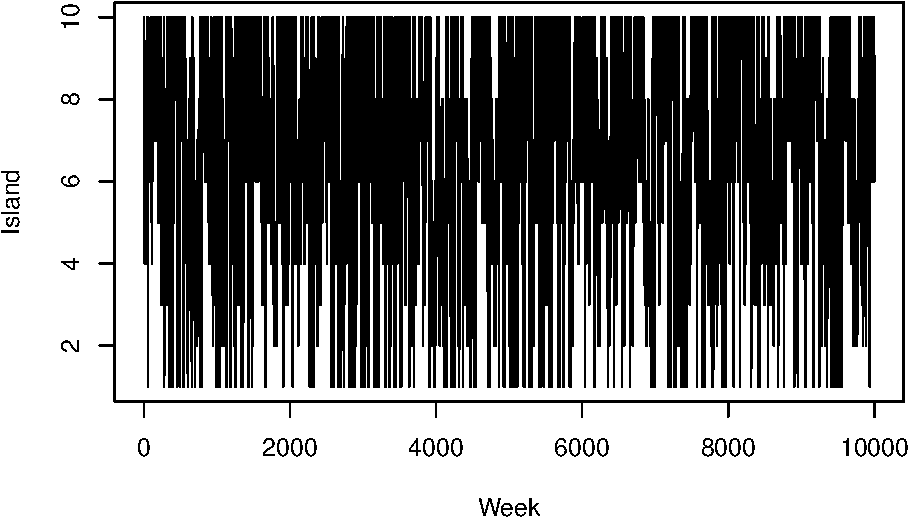
\includegraphics{_main_files/figure-latex/unnamed-chunk-27-1.pdf}
\end{example}

\hypertarget{advanced-computation}{%
\chapter{Advanced Computation}\label{advanced-computation}}

Now we have the tools of Bayesian inference and methods to sample from complex posterior distributions, we can start to look at more advanced methods and models. This chapter is split into two distinct parts, each showing a different method in Bayesian inference.

\hypertarget{data-augmentation}{%
\section{Data Augmentation}\label{data-augmentation}}

Real world data are often messy with data points missing which may mean they are partially or completely unobserved. One common example of this is in clinical trials where people drop out of the trial before their treatment is complete. Another example is crime data, where only a fraction of crimes are reported and many crimes go unobserved. Two common ways to deal with partially or completely unobserved are:

\begin{itemize}
\tightlist
\item
  Remove data points that are not completely observed. This throws away information and is likely to increase the overall uncertainty in the estimates.
\item
  Replace data points that are not completely observed with estimates such as the sample mean. This is likely to underestimate the uncertainty as we are treating the observation as completely observed when it is not.
\end{itemize}

The Bayesian framework provides a natural way for dealing with missing, partially, or completely unobserved data. It allows us to treat the missing data points as random variables and infer the data points alongside the model parameters. This provides us with a method to quantify the uncertainty around our estimates of the missing data points.

In data augmentation, we distinguish between two likelihood functions.

\begin{definition}
The \textbf{observed data likelihood function} is the likelihood function of the observed data.
\end{definition}

\begin{definition}
The \textbf{complete data likelihood function} is the likelihood function of the observed data and any missing or censored data had they been fully observed.
\end{definition}

The difference between the two likelihood functions is that the complete data likelihood function is the functions had we observed everything we want to observe. However, as the complete data likelihood function contains data we didn't fully observe, we can't compute it. Instead we can only evaluate the observed data likelihood function. A simple probability based example of this is if there are two events \(X\) and \(Y\), where the outcome of \(X\) is observed and \(Y\) unobserved. The complete data likelihood is \(pi(X = x, Y = y)\) because we are considering all the events, observed or not. However, we can only compute \(\pi(x) = \int_{y \in Y}\pi(X = x, Y = y)\) or \(\pi(x) = \sum_{y \in Y}\pi(X = x, Y = y)\), since \(y\) is unobserved.

In data augmentation, we start off with the observed data likelihood function and then augment this function by introducing variables that we want to have fully observed. This then gives us the complete data likelihood function.

\hypertarget{imputing-censored-observations}{%
\subsection{Imputing censored observations}\label{imputing-censored-observations}}

The first example we will look at is when data is censored. Instead of throwing away these observations, we will instead treat them as random variables and infer their values.

\begin{example}
A bank checks transactions for suspicious activities in batches of 1000. Denote the probability a transaction is suspicious by \(p\) and the number of suspicious transactions in a batch by \(Y\).

The bank checks five batches and observes \(y_1, \ldots, y_4\) suspicious transactions in the first four batches. Due to a computer error, the number of suspicious transactions in the final batch is not properly recorded, but is known to be less than 6.

The observed data likelihood functions is
\[
\pi(y_1, \ldots, y_4, \tilde{y}_5 \mid p) = \left(\prod_{i=1}^4\begin{pmatrix} 1000 \\ y_i \end{pmatrix} p^{y_i}(1-p)^{1000 - y_i} \right)\left(\sum_{j=0}^5\begin{pmatrix} 1000 \\ j \end{pmatrix} p^{j}(1-p)^{1000 - j}\right).
\]
This is known as marginalising over the missing variable, just as we did in the simple probability example earlier. Placing a uniform prior distribution on \(p \sim U[0, 1]\) give the posterior distribution
\[
\pi(p, \tilde{y}_5 \mid y_1, \ldots, y_4)= \left(\prod_{i=1}^4\begin{pmatrix} 1000 \\ y_i \end{pmatrix} p^{y_i}(1-p)^{y_i} \right)\left(\sum_{j=0}^5\begin{pmatrix} 1000 \\ j \end{pmatrix} p^{j}(1-p)^{1000 - j}\right).
\]
Although we could sample from this distribution, it is not easy to work with. Instead, we can write down the complete data likelihood. Suppose that \(y_5\) was observed, then the complete data likelihood may be written as
\[
\pi(y_1, \ldots, y_5 \mid p)  = \prod_{i=1}^5\begin{pmatrix} 1000 \\ y_i \end{pmatrix} p^{y_i}(1-p)^{1000 - y_i},
\]
The posterior distribution is therefore
\[
p \mid y_1, \ldots, y_5 \sim \hbox{Beta}\left(\sum_{i=1}^5 y_i + 1, 1001 - \sum_{i=1}^5 y_i\right).
\]

The full conditional distribution of \(y_5\) given \(p\), the other data points an \(y_5 < 6\) is
\[
  \pi(y_5 = y \mid y_1, \ldots, y_4, y_5 < 1, p) = \frac{\begin{pmatrix} 1000 \\ y \end{pmatrix} p^{y}(1-p)^{1000 - y}}{\sum_{j=0}^{1000}\begin{pmatrix} 1000 \\ j \end{pmatrix} p^{j}(1-p)^{j}}, \qquad y < 6
\]
We can use a Gibbs sampler alternating between sampling \(p\) and \(y_5\).
\end{example}

\hypertarget{imputing-latent-variables}{%
\subsection{Imputing Latent Variables}\label{imputing-latent-variables}}

Often there are variables that are cannot be observed, these may be hidden somehow or introduced to help with the modelling. Instead we can learn about this variable indirectly from the data.

A \textbf{latent variable} is a variable that cannot be observed.

A mixture model is an example of latent variables being useful.

\begin{example}

Royal Mail use image detection software to read postcodes on letters. A camera scans the front of an envelope and then records the barcode. This example is a very simplified version of how the system could work.

Suppose the machine is processing a bag of letters addressed to people in either B1 or B2 postcodes. The camera scans the first two characters of the postcode (B1 or B2) and records the proportion of the scanned image that is taken up by the characters. The picture below shows an example of what the scanned image looks like.

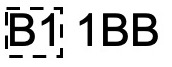
\includegraphics{postcode.jpeg}

We introduce a latent variable \(z_i \sim \hbox{Bernoulli}(p)\) that describes if the characters on the \(i^{th}\) image are B1 or B2. The observation \(y_i\) is the proportion of the \(i^{th}\) image that is taken up by the characters. We observe \(y_i\), but want to estimate \(z_i\). The difficultly is there lack of one-to-one correspondence between the values \(y_i\) can take and the value \(z_i\). Due to the different handwriting and fonts used on envelopes, if the letter is going to B1 (\(Z = 1\)), then \(Y_i \sim N(0.7, 0.05^2)\) and if it is going to B2 (\(Z = 2\)), then \(Y_i \sim N(0.8, 0.02^2)\). The plot below shows the two densities and the overlap between them.

\begin{Shaded}
\begin{Highlighting}[]
\NormalTok{a }\OtherTok{\textless{}{-}} \FunctionTok{seq}\NormalTok{(}\FloatTok{0.5}\NormalTok{, }\FloatTok{0.9}\NormalTok{, }\FloatTok{0.001}\NormalTok{)}
\NormalTok{x }\OtherTok{\textless{}{-}} \FunctionTok{dnorm}\NormalTok{(a, }\FloatTok{0.7}\NormalTok{, }\FloatTok{0.05}\NormalTok{)}
\NormalTok{y }\OtherTok{\textless{}{-}} \FunctionTok{dnorm}\NormalTok{(a, }\FloatTok{0.8}\NormalTok{, }\FloatTok{0.02}\NormalTok{)}
\FunctionTok{plot}\NormalTok{(a, x, }\AttributeTok{type =} \StringTok{\textquotesingle{}l\textquotesingle{}}\NormalTok{, }\AttributeTok{ylim =} \FunctionTok{c}\NormalTok{(}\DecValTok{0}\NormalTok{, }\DecValTok{20}\NormalTok{), }\AttributeTok{xlab =} \FunctionTok{expression}\NormalTok{(y), }\AttributeTok{ylab =} \StringTok{"density"}\NormalTok{)}
\FunctionTok{lines}\NormalTok{(a, y, }\AttributeTok{lty =} \DecValTok{2}\NormalTok{)}
\end{Highlighting}
\end{Shaded}

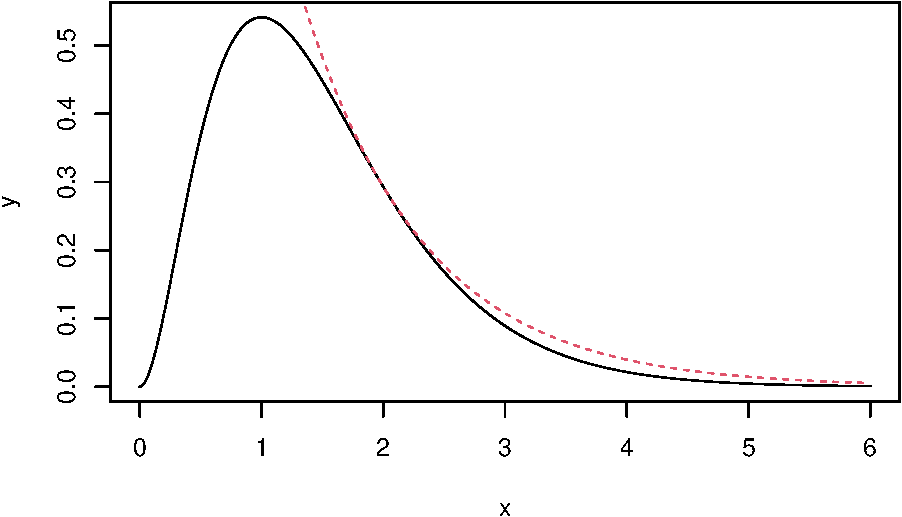
\includegraphics{_main_files/figure-latex/unnamed-chunk-29-1.pdf}

As the variables \(\boldsymbol{z}\) are latent, the observed data likelihood function is
\[
\pi(\boldsymbol{y} \mid  p) =\prod_{i=1}^N \left[ p\pi(y_i \mid \mu = 0.7, \sigma^2 = 0.05^2) + (1-p)\pi(y_i \mid \mu = 0.8, \sigma^2 = 0.02^2)\right].
\]
Instead, it's easier to work with the complete data likelihood function, supposing we had observed the variables \(\boldsymbol{z}\). This is given by
\begin{align*}
\pi(\boldsymbol{y}, \boldsymbol{z} \mid  p) &= \begin{pmatrix} N_1 + N_2
\\ N_1\end{pmatrix}p^{N_1}(1-p)^{N_2} \prod_{i; z_i = 1}\pi(y_i \mid \mu = 0.7, \sigma^2 = 0.05^2)  \\
&\times\prod_{i; z_i = 2}\pi(y_i \mid \mu = 0.8, \sigma^2 = 0.02^2),
\end{align*}
where \(N_1\) and \(N_2\) are the number of letters for B1 and B2 respectively. This form makes it much easier to derive the posterior distributions and estimate the parameter values.

We place a uniform prior distribution on the parameter \(p\), which gives the posterior distribution
\[
p \mid \boldsymbol{y}, \boldsymbol{z} \sim \hbox{Beta}(N_1 + 1, N_2 + 1).
\]

The distribution of \(z_i\) given the parameter \(p\) and the observation \(y_i\) can be derived using Bayes' theorem
\[
p^*_i = \pi(z = 1 \mid p, y_1) = \frac{p\pi(y_i \mid \mu = 0.7, \sigma^2 = 0.05^2)}{p\pi(y_i \mid \mu = 0.7, \sigma^2 = 0.05^2) + (1-p)\pi(y_i \mid \mu = 0.8, \sigma^2 = 0.02^2)}.
\]
The full conditional distribution is therefore \(z_i \mid \boldsymbol{y}, p \sim \hbox{Bernoulli}(p^*_i)\).

An MCMC algorithm for this would repeat the following two steps:

\begin{enumerate}
\def\labelenumi{\arabic{enumi}.}
\tightlist
\item
  Sample \(p \mid \boldsymbol{y}, \boldsymbol{z} \sim \hbox{Beta}(N_1 + 1, N_2 + 1)\).
\item
  Sample \(z_i \mid \boldsymbol{y}, p \sim \hbox{Bernoulli}(p^*_i)\) for each \(i\).
\end{enumerate}

\end{example}

\hypertarget{gaussian-processes}{%
\section{Gaussian Processes}\label{gaussian-processes}}

So far in the module, we have considered prior distribution on parameters. These parameters have taken values (mostly real) or real-valued vectors. In this section, we're going to extend this idea further to place prior distributions on functions. That is, we're going to describe a prior distribution that when sampled gives us functions. The method we're going to use is called a Gaussian Process (GP).

Before, we define a GP, we're going to build an intuitive definition of it. Recall the normal distribution with mean \(\mu\) and variance \(\sigma^2\), \(N(\mu, \sigma^2)\). It assigns probabilities to values on the real line -- when we sample from it, we get real values. The plot below shows the density function for a \(N(0, 1)\) distribution and five samples.

\begin{Shaded}
\begin{Highlighting}[]
\CommentTok{\#Plot N(0, 1)}
\NormalTok{x }\OtherTok{\textless{}{-}} \FunctionTok{seq}\NormalTok{(}\SpecialCharTok{{-}}\DecValTok{4}\NormalTok{, }\DecValTok{4}\NormalTok{, }\FloatTok{0.01}\NormalTok{)}
\NormalTok{y }\OtherTok{\textless{}{-}} \FunctionTok{dnorm}\NormalTok{(x)}
\FunctionTok{plot}\NormalTok{(x, y, }\AttributeTok{type =} \StringTok{\textquotesingle{}l\textquotesingle{}}\NormalTok{)}

\CommentTok{\#Add samples}
\NormalTok{samples }\OtherTok{\textless{}{-}} \FunctionTok{rnorm}\NormalTok{(}\DecValTok{5}\NormalTok{)}
\FunctionTok{rug}\NormalTok{(samples)}
\end{Highlighting}
\end{Shaded}

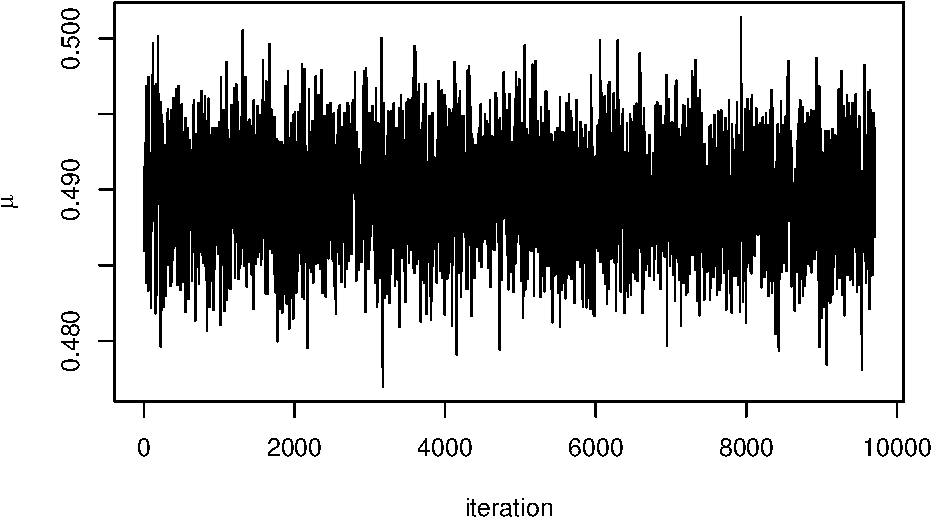
\includegraphics{_main_files/figure-latex/unnamed-chunk-30-1.pdf}

The multivariate normal distribution extends this to a vector space, \(\mathbb{R}^N\). Instead of having a mean and variance value, the distribution is defined through a mean vector and covariance matrix. The mean vector describes the expected value of each component of the vector and the covariance matrix describes the relationship between each pair of components in the vector. When we draw samples, we get vectors. The plot below shows the density of the multivariate normal distribution with \(N = 2\), zero mean, \(\sigma^2_x = \sigma^2_y = 1\) and \(\rho = 0.7\).

\begin{Shaded}
\begin{Highlighting}[]
\CommentTok{\#Create Grid}
\NormalTok{x }\OtherTok{\textless{}{-}} \FunctionTok{seq}\NormalTok{(}\SpecialCharTok{{-}}\DecValTok{3}\NormalTok{,}\DecValTok{3}\NormalTok{,}\AttributeTok{length.out=}\DecValTok{100}\NormalTok{)}
\NormalTok{y }\OtherTok{\textless{}{-}} \FunctionTok{seq}\NormalTok{(}\SpecialCharTok{{-}}\DecValTok{3}\NormalTok{,}\DecValTok{3}\NormalTok{,}\AttributeTok{length.out=}\DecValTok{100}\NormalTok{)}

\CommentTok{\#Evaluate density at grid}
\NormalTok{z }\OtherTok{\textless{}{-}} \FunctionTok{matrix}\NormalTok{(}\DecValTok{0}\NormalTok{,}\AttributeTok{nrow=}\DecValTok{100}\NormalTok{,}\AttributeTok{ncol=}\DecValTok{100}\NormalTok{)}
\NormalTok{mu }\OtherTok{\textless{}{-}} \FunctionTok{c}\NormalTok{(}\DecValTok{0}\NormalTok{,}\DecValTok{0}\NormalTok{)}
\NormalTok{sigma }\OtherTok{\textless{}{-}} \FunctionTok{matrix}\NormalTok{(}\FunctionTok{c}\NormalTok{(}\DecValTok{1}\NormalTok{, }\FloatTok{0.7}\NormalTok{, }\FloatTok{0.7}\NormalTok{, }\DecValTok{1}\NormalTok{),}\AttributeTok{nrow=}\DecValTok{2}\NormalTok{)}
\ControlFlowTok{for}\NormalTok{ (i }\ControlFlowTok{in} \DecValTok{1}\SpecialCharTok{:}\DecValTok{100}\NormalTok{) \{}
  \ControlFlowTok{for}\NormalTok{ (j }\ControlFlowTok{in} \DecValTok{1}\SpecialCharTok{:}\DecValTok{100}\NormalTok{) \{}
\NormalTok{    z[i,j] }\OtherTok{\textless{}{-}}\NormalTok{ mvtnorm}\SpecialCharTok{::}\FunctionTok{dmvnorm}\NormalTok{(}\FunctionTok{c}\NormalTok{(x[i],y[j]),}
                      \AttributeTok{mean=}\NormalTok{mu,}\AttributeTok{sigma=}\NormalTok{sigma)}
\NormalTok{  \}}
\NormalTok{\}}

\CommentTok{\#Generate contour plot}
\FunctionTok{contour}\NormalTok{(x, y ,z)}
\end{Highlighting}
\end{Shaded}

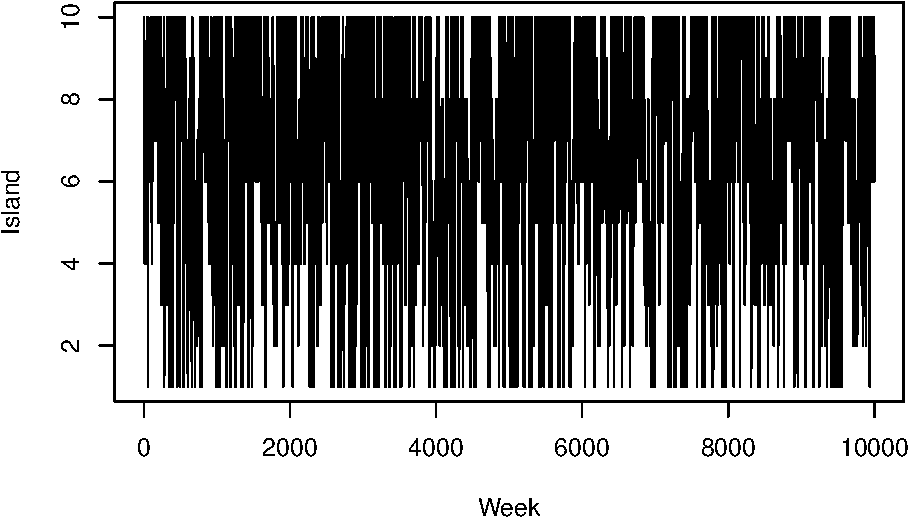
\includegraphics{_main_files/figure-latex/unnamed-chunk-31-1.pdf}

A GP takes this one step further and puts a prior distribution on a function space. It is specified by a mean function, \(\mu(\cdot)\) and covariance function \(k(\cdot, \cdot)\). The mean function describes the expected value of each point the function can be evaluated at, and the covariance function describes the relationship between each point on the function. The plot below shows three samples from a GP distribution with mean function the zero function \(\mu(x) = 0\, \forall x\) and a covariance function that supports smooth functions.

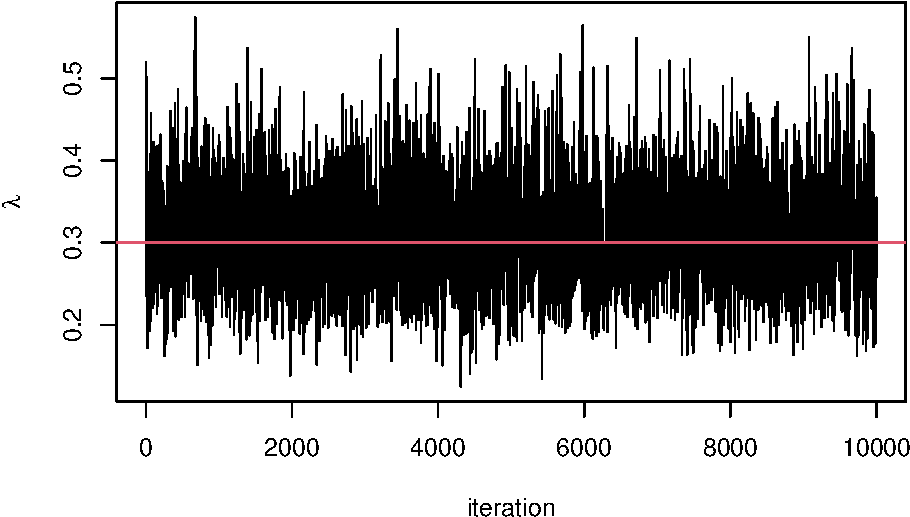
\includegraphics{_main_files/figure-latex/unnamed-chunk-32-1.pdf}

\begin{definition}
A \textbf{Gaussian Process} is a collection of random variables, any finite number of which have a joint Gaussian distribution.
\end{definition}

This says that is we think of a function as an infinite collection of points, then if any finite subset of those points following a Gaussian distribution, we have a Gaussian process. In reality, we set up the function so that is meets this definition. More formally,

\begin{definition}
A \textbf{GP distribution on a function \(f(x)\)} is defined through its mean function \(\mu(x) = \mathbb{E}(x)\) and covariance function \(k(x, x') = \mathbb{E}(x)\left((f(x) - \mu(x))(f(x') - \mu(x'))\right)\). We write it as \(f(x) \sim \mathcal{GP}(\mu(x), k(x, x'))\).
\end{definition}

Before we go any further, it is worth proceeding with caution. Those with good memories, we recall Bernstein-von-Mises' theorem from Chapter 3.

\begin{theorem}[Bernstein-von-Mises]
For a well-specified model \(\pi(\boldsymbol{y} \mid \theta)\) with a fixed number of parameters, and for a smooth prior distribution \(\pi(\theta)\) that is non-zero around the MLE \(\hat{\theta}\), then
\[
\left|\left| \pi(\theta \mid \boldsymbol{y}) - N\left(\hat{\theta}, \frac{I(\hat{\theta})^{-1}}{n}\right) \right|\right|_{TV} \rightarrow 0.
\]
\end{theorem}

Bernstein-von-Mises' theorem only holds when the model has a fixed (i.e.~finite) number of parameters. A GP is defined on an infinite collection of points, and so this theorem does not hold. This is the first time in this module we have encountered a distribution where Bernstein-von-Mises' theorem does not hold. Fortunately, various forms of Bernstein-von-Mises' theorems for GPs exist, with many coming about in the early 2010s. However, this is still an ongoing area of research.

\hypertarget{covariance-functions}{%
\subsection{Covariance Functions}\label{covariance-functions}}

One issue when using GPs is describing the covariance function. How do we decide how each pair of points (there being an infinite number of them)? There are lots of standard choices of covariance functions that we can choose from, each one making different assumptions about the function we are interested in.

The most common covariance function is the squared exponential functions. It is used to model functions that are `nice', i.e.~they are smooth, continuous and infinitely differentiable.

\begin{definition}
The \textbf{squared exponential covariance function} takes the form
\[
k(x, x') = \alpha^2\exp\left\{-\frac{1}{l}(x-x')^2\right\},
\]
where \(\alpha^2\) is the signal variance and \(l>0\) is the length scale parameter.
\end{definition}

For now, consider \(\alpha = l = 1\). What is the covariance between the function evaluated at 0 and the function evaluated at \(x\)? The plot below shows the covariance.

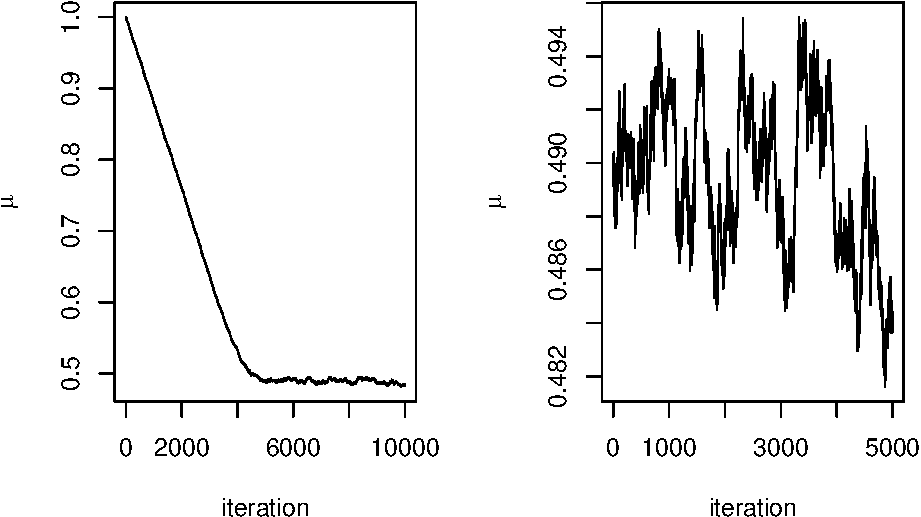
\includegraphics{_main_files/figure-latex/unnamed-chunk-33-1.pdf}

The covariance is highest when the \(x\) is near to 0, i.e.~the points are immediately next to each other. If the value of \(x\) is \(\pm 2\), the covariance is 0. As we are dealing with a joint normal distribution, a covariance of 0 implies independence. So with this covariance function, the value of \(f(x)\) is independent of \(f(0)\) if \(|x|\) is larger than about two. The parameter \(l\) is called the length scale parameter and dictates how quickly the covariance decays. Small values of \(l\) mean that the value of the function at nearby points are independent of each other, resulting in functions that look like white noise. Large values of \(l\) mean that even if points are far away, they are still highly dependent on each other. This gives very flat functions.

The squared exponential covariance function produces functions that are continuous and differentiable. There are many other types of covariance functions, including ones that don't produce functions that are continuous or differentiable. Two more are given below.

\begin{definition}
The \textbf{M\textquotesingle atern covariance function} models functions that are differentiable only once:
\[
k(x, x') = \left(1 + \frac{\sqrt{3}(x - x')^2}{l} \right)\exp\left\{-\frac{\sqrt{3}(x - x')^2}{l} \right\}.
\]
\end{definition}

\begin{definition}
The periodic covariance function models functions that are periodic and it is given by
\[
k(x, x') = \alpha^2 \exp\left\{-\frac{2}{l}\sin^2\frac{(x-x')^2}{p} \right\},
\]
where the period is \(p\).
\end{definition}

\hypertarget{gaussian-process-regression}{%
\subsection{Gaussian Process Regression}\label{gaussian-process-regression}}

One of the main applications of GPs in in regression. Suppose we observe the points below \(\boldsymbol{y} = \{y_1, \ldots, y_N\}\) and want to fit a curve through them. One method is to write down a set of functions of the form \(\boldsymbol{y} = X^T\boldsymbol{\beta} + \boldsymbol{\varepsilon}\), where \(X\) is the design matrix and \(\boldsymbol{\beta}\) a vector of parameters. For each design matrix \(X\), construct the posterior distributions for \(\boldsymbol{\beta}\) and use some goodness-of-fit measure to choose the most suitable design matrix.

\begin{Shaded}
\begin{Highlighting}[]
\NormalTok{x }\OtherTok{\textless{}{-}} \SpecialCharTok{{-}}\DecValTok{5}\SpecialCharTok{:}\DecValTok{5}
\NormalTok{y }\OtherTok{\textless{}{-}} \FunctionTok{sin}\NormalTok{(x}\SpecialCharTok{/}\DecValTok{2}\NormalTok{)}\SpecialCharTok{\^{}}\DecValTok{2} \SpecialCharTok{+} \FunctionTok{exp}\NormalTok{(}\SpecialCharTok{{-}}\NormalTok{x}\SpecialCharTok{/}\DecValTok{5}\NormalTok{) }\SpecialCharTok{+} \FunctionTok{rnorm}\NormalTok{(}\FunctionTok{length}\NormalTok{(x), }\DecValTok{0}\NormalTok{, }\FloatTok{0.2}\NormalTok{)}
\FunctionTok{plot}\NormalTok{(x, y)}
\end{Highlighting}
\end{Shaded}

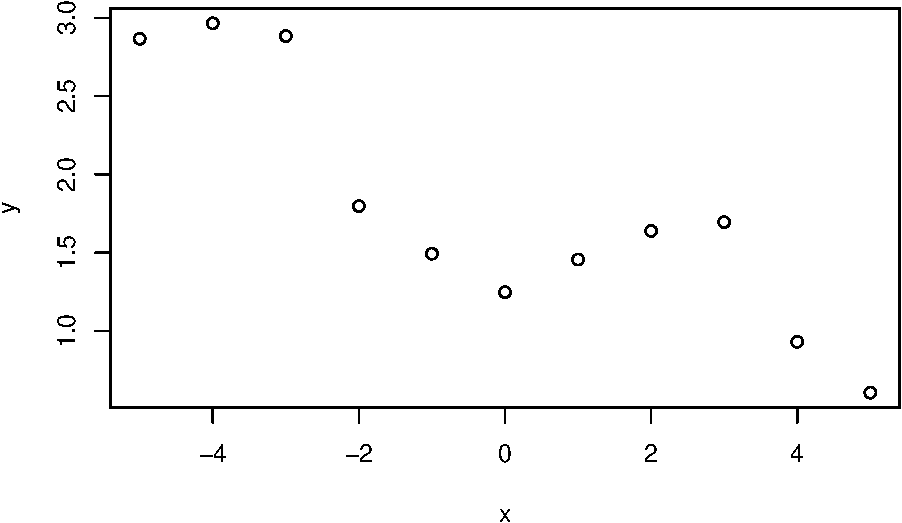
\includegraphics{_main_files/figure-latex/unnamed-chunk-34-1.pdf}

One difficulty is writing down the design matrices \(X\), it is often not straightforward to propose or justify these forms GPs allow us to take a much less arbitrary approach, simply saying that \(y_i = f(x_i) + \varepsilon_i\) and placing a GP prior distribution on \(f\).

Although we're placing an prior distribution with an infinite dimension on \(f\), we only ever need to work with a finite dimensional object, making this much easier. We only observe the function at finite number of points \(\boldsymbol{f} = \{f(x_1), \ldots, f(x_N)\}\) and we will infer the value of the function at points on a fine grid, \(\boldsymbol{f}^* = \{f(x_1^*), \ldots, f(x_N^*)\}\). By the definition of a GP, the distribution of these points is a multivariate normal distribution.

\begin{example}
Suppose we observe \(\boldsymbol{y} = \{y_1, \ldots, y_N\}\) at \(\boldsymbol{x} = \{x_1, \ldots, x_N\}\). The plot below shows these points.

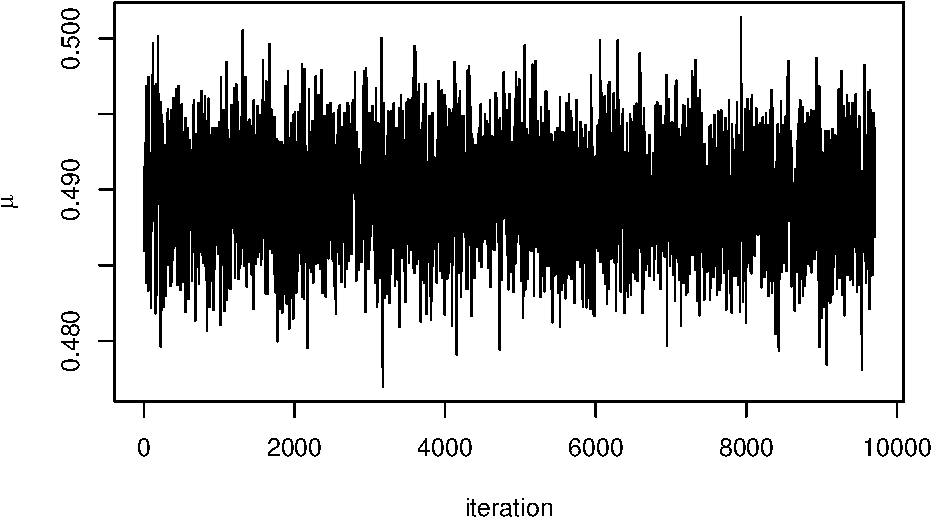
\includegraphics{_main_files/figure-latex/unnamed-chunk-35-1.pdf}

Using the model \(y_i = f(x_i) + \varepsilon_i\), where \(\varepsilon_i \sim N(0, \sigma^2)\), we want to infer the function \(f\) evaluated at a gird of points \(\boldsymbol{f}^* = \{f(x_1^*), \ldots, f(x_N^*)\}\). We place a GP prior distribution on \(f \sim \mathcal{GP}(0, k)\), where \(k\) is the squared exponential covariance function. Using the model, the covariance between points \(y_i\) and \(y_j\) is
\[
\textrm{cov}(y_i, y_j) = k(x_i, x_j) + \sigma^21_{i=j}.
\]
That is the covariance function evaluated at \(x_i\) and \(x_j\) plus \(\sigma^2\) if \(i = j\). We can write this in matrix form as \(K(\boldsymbol{x}, \boldsymbol{x}) + \sigma^2I\) where \(I\) is the identity matrix. The distribution of \(\boldsymbol{y}\) is therefore \(\boldsymbol{y} \sim N(\boldsymbol{0}, \, K(\boldsymbol{x}, \boldsymbol{x}) + \sigma^2I)\). By definition of the GP, the distribution of the function evaluated at the fine grid is \(\boldsymbol{f}^* \sim N(\boldsymbol{0}, K(\boldsymbol{x}^*, \boldsymbol{x}^*))\).

We can now write the joint distribution as
\[
\begin{pmatrix}
\boldsymbol{y} \\
\boldsymbol{f}^*
\end{pmatrix} \sim N\left(\boldsymbol{0}, \,
\begin{pmatrix}
 K(\boldsymbol{x}, \boldsymbol{x}) + \sigma^2I &  K(\boldsymbol{x}, \boldsymbol{x}^*)\\
K(\boldsymbol{x}^*, \boldsymbol{x}) & K(\boldsymbol{x}^*, \boldsymbol{x}^*)
\end{pmatrix}.
\right)
\]
The off-diagonal terms in the covariance matrix describe the relationship between the observed points \(\boldsymbol{y}\) and the points of interest \(\boldsymbol{f}^*\). We can now write down the distribution of \(\boldsymbol{f}^*\) given the observed points \(\boldsymbol{y}\) and \(\sigma^2\).
\[
\boldsymbol{f}^* \mid \boldsymbol{y}, \sigma^2 \sim N(\boldsymbol{\mu}^*, \, K^*),
\]
where \(\boldsymbol{\mu}^* = K(\boldsymbol{x}^*, \boldsymbol{x})(K(\boldsymbol{x}, \boldsymbol{x}) + \sigma^2 I)^{-1} \boldsymbol{y}\) and \(K^* = K(\boldsymbol{x}^*, \boldsymbol{x}^*) - K(\boldsymbol{x}^*, \boldsymbol{x})(K(\boldsymbol{x}, \boldsymbol{x}) + \sigma^2I)^{-1}K(\boldsymbol{x}, \boldsymbol{x}^*)\).

We set the fine gird to be \(\boldsymbol{x}^* = \{-5, -4.99, -4.98, \ldots, 5\}\), the GP parameters \(\alpha = l = 1\) and \(\sigma = 0.2\). The posterior mean and 95\% credible interval are shown below.
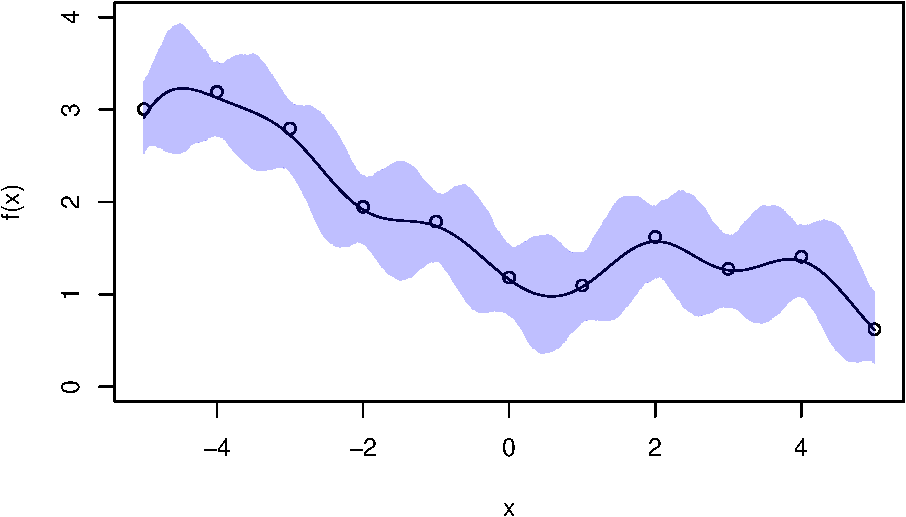
\includegraphics{_main_files/figure-latex/unnamed-chunk-36-1.pdf}
The posterior mean for \(f\) is a smooth line passing near each point. The 95\% credible interval for \(f\) has the smallest variance near each point, and largest furthest away from the points.
\end{example}

\hypertarget{lab-data-augmenatation}{%
\section{Lab: Data Augmenatation}\label{lab-data-augmenatation}}

\hypertarget{lab-gaussian-processes}{%
\section{Lab: Gaussian Processes}\label{lab-gaussian-processes}}

  \bibliography{book.bib,packages.bib}

\end{document}
